% ============================================================================
%  Doc L -- SPEAR3 RF System: Legacy System Architecture
%  Build:  powershell -ExecutionPolicy Bypass -File build.ps1
%  Engine: LuaLaTeX (required -- see the Unicode note in preamble.tex)
% ============================================================================
\documentclass[letterpaper,11pt]{article}
% ============================================================================
%  SPEAR3 RF System documentation -- shared preamble
%  Engine: LuaLaTeX.  Build with build.ps1 (latexmk -lualatex).
% ============================================================================

\usepackage[letterpaper,top=1in,bottom=1in,left=1.05in,right=1.05in]{geometry}

% --- fonts -----------------------------------------------------------------
\usepackage{fontspec}
\setmainfont{TeX Gyre Termes}
\setsansfont{TeX Gyre Heros}
\setmonofont{Consolas}[Scale=0.86]

% --- Unicode safety --------------------------------------------------------
% LuaLaTeX DROPS unmapped glyphs SILENTLY -- an unmapped U+03BC turns "8 uF"
% into "8 F".  Every non-ASCII character used in these documents is mapped
% here.  The build script fails if the log reports "Missing character".
\usepackage{newunicodechar}
\newunicodechar{μ}{\ensuremath{\mu}}      \newunicodechar{µ}{\ensuremath{\mu}}
\newunicodechar{Ω}{\ensuremath{\Omega}}   \newunicodechar{≈}{\ensuremath{\approx}}
\newunicodechar{≥}{\ensuremath{\geq}}     \newunicodechar{≤}{\ensuremath{\leq}}
\newunicodechar{≠}{\ensuremath{\neq}}     \newunicodechar{×}{\ensuremath{\times}}
\newunicodechar{÷}{\ensuremath{\div}}     \newunicodechar{±}{\ensuremath{\pm}}
\newunicodechar{−}{\ensuremath{-}}        \newunicodechar{√}{\ensuremath{\sqrt{}}}
\newunicodechar{α}{\ensuremath{\alpha}}   \newunicodechar{β}{\ensuremath{\beta}}
\newunicodechar{φ}{\ensuremath{\varphi}}  \newunicodechar{ω}{\ensuremath{\omega}}
\newunicodechar{Δ}{\ensuremath{\Delta}}   \newunicodechar{τ}{\ensuremath{\tau}}
\newunicodechar{θ}{\ensuremath{\theta}}   \newunicodechar{λ}{\ensuremath{\lambda}}
\newunicodechar{π}{\ensuremath{\pi}}      \newunicodechar{σ}{\ensuremath{\sigma}}
\newunicodechar{₀}{\ensuremath{_0}}       \newunicodechar{₁}{\ensuremath{_1}}
\newunicodechar{₂}{\ensuremath{_2}}       \newunicodechar{²}{\ensuremath{^2}}
\newunicodechar{³}{\ensuremath{^3}}       \newunicodechar{⁴}{\ensuremath{^4}}
\newunicodechar{⁻}{\ensuremath{^-}}       \newunicodechar{⁺}{\ensuremath{^+}}
\newunicodechar{→}{\ensuremath{\rightarrow}}
\newunicodechar{←}{\ensuremath{\leftarrow}}
\newunicodechar{↔}{\ensuremath{\leftrightarrow}}
\newunicodechar{⇒}{\ensuremath{\Rightarrow}}
\newunicodechar{⊕}{\ensuremath{\oplus}}   \newunicodechar{∥}{\ensuremath{\parallel}}
\newunicodechar{°}{\ensuremath{^\circ}}   \newunicodechar{·}{\ensuremath{\cdot}}
\newunicodechar{≪}{\ensuremath{\ll}}      \newunicodechar{≫}{\ensuremath{\gg}}
\newunicodechar{✓}{\checkmark}            \newunicodechar{⚠}{\textbf{!}}
\newunicodechar{–}{--}                    \newunicodechar{—}{---}

% --- maths and units -------------------------------------------------------
\usepackage{amsmath,amssymb}
\usepackage{siunitx}
\DeclareSIUnit\voltampere{VA}
\DeclareSIUnit\VAR{var}
% range-phrase must not rely on literal spaces (LaTeX strips them from a key
% value, so "{ to }" renders as "10to20") and must force text mode (siunitx
% sets numbers in math, where a bare "--" becomes two minus signs).
\sisetup{per-mode=symbol,range-phrase={\text{--}},range-units=single,
         group-minimum-digits=4,detect-weight=true}

% --- tables ----------------------------------------------------------------
\usepackage{longtable,booktabs,array,tabularx,multirow}
\usepackage{ragged2e}
\setlength{\LTleft}{0pt}\setlength{\LTright}{0pt}
\renewcommand{\arraystretch}{1.18}
% left-aligned, hyphenating paragraph column used by every wide table
\newcolumntype{P}[1]{>{\RaggedRight\arraybackslash}p{#1}}
% Same, but \small: for dense tables.  The size must live in the column type --
% wrapping a longtable in {\small ...} breaks its page-breaking \write.
\newcolumntype{Q}[1]{>{\small\RaggedRight\arraybackslash}p{#1}}

% --- graphics and figures --------------------------------------------------
\usepackage{graphicx}
% Resolved from the document's own folder, which is the working directory.
\graphicspath{{../common/}{../common/photos/}{../common/generated/}}
\usepackage{float}
\usepackage[font=small,labelfont=bf,width=0.92\linewidth]{caption}
\usepackage{comment}

% A figure must not drift out of the section it belongs to.  With 47 floats
% LaTeX will otherwise push them pages away from the text that discusses them.
\usepackage[section]{placeins}

% Default float parameters are tuned for papers with two or three figures.
% This document is figure-dense, so allow more of a page to be float and more
% floats per page; without this, figures queue up and drift several pages.
\renewcommand{\topfraction}{0.88}
\renewcommand{\bottomfraction}{0.70}
\renewcommand{\textfraction}{0.10}
\renewcommand{\floatpagefraction}{0.72}
\setcounter{topnumber}{3}
\setcounter{bottomnumber}{2}
\setcounter{totalnumber}{5}

% Image size policy.  Photographs are capped in BOTH width and height so that
% no figure can ever exceed roughly half a page, whatever its aspect ratio.
\newlength{\photomaxh}\setlength{\photomaxh}{0.34\textheight} % ~1/3 page
\newlength{\widemaxh} \setlength{\widemaxh}{0.46\textheight}  % ~1/2 page

% \photofig{file}{caption}{label}      -- default, about 1/3 page
\newcommand{\photofig}[3]{%
  \begin{figure}[htbp]\centering
    \includegraphics[width=0.62\linewidth,height=\photomaxh,keepaspectratio]{#1}%
    \caption{#2}\label{#3}
  \end{figure}}
% \widefig{file}{caption}{label}       -- for detailed schematics, about 1/2 page
\newcommand{\widefig}[3]{%
  \begin{figure}[htbp]\centering
    \includegraphics[width=0.94\linewidth,height=\widemaxh,keepaspectratio]{#1}%
    \caption{#2}\label{#3}
  \end{figure}}
% \smallfig{file}{caption}{label}      -- for low-resolution sources
\newcommand{\smallfig}[3]{%
  \begin{figure}[htbp]\centering
    \includegraphics[width=0.44\linewidth,height=0.26\textheight,keepaspectratio]{#1}%
    \caption{#2}\label{#3}
  \end{figure}}
% \tallfig{file}{caption}{label}       -- portrait-orientation photographs.
% A tall photo capped at \photomaxh comes out only ~45 mm wide, so these are
% capped by height instead and allowed a narrower column.
\newcommand{\tallfig}[3]{%
  \begin{figure}[tbp]\centering
    \includegraphics[width=0.46\linewidth,height=0.50\textheight,keepaspectratio]{#1}%
    \caption{#2}\label{#3}
  \end{figure}}
% two portrait photographs side by side under one caption:
% \tallpairfig{fileA}{subA}{labA}{fileB}{subB}{labB}{caption}{label}
\newcommand{\tallpairfig}[8]{%
  \begin{figure}[tbp]\centering
    \begin{minipage}[b]{0.46\linewidth}\centering
      \includegraphics[width=\linewidth,height=0.40\textheight,keepaspectratio]{#1}%
      \subcaption{#2}\label{#3}
    \end{minipage}\hfill
    \begin{minipage}[b]{0.46\linewidth}\centering
      \includegraphics[width=\linewidth,height=0.40\textheight,keepaspectratio]{#4}%
      \subcaption{#5}\label{#6}
    \end{minipage}
    \caption{#7}\label{#8}
  \end{figure}}
% two photographs side by side, each about 1/4 page
\newcommand{\pairfig}[6]{%
  \begin{figure}[htbp]\centering
    \begin{minipage}[t]{0.48\linewidth}\centering
      \includegraphics[width=\linewidth,height=0.26\textheight,keepaspectratio]{#1}%
      \subcaption{#2}\label{#3}
    \end{minipage}\hfill
    \begin{minipage}[t]{0.48\linewidth}\centering
      \includegraphics[width=\linewidth,height=0.26\textheight,keepaspectratio]{#4}%
      \subcaption{#5}\label{#6}
    \end{minipage}
  \end{figure}}
\usepackage{subcaption}

% --- diagrams --------------------------------------------------------------
\usepackage{tikz}
\usetikzlibrary{arrows.meta,positioning,fit,backgrounds,calc,shapes.geometric,
                shapes.misc,chains,decorations.pathreplacing,patterns,matrix}
\usepackage{pgfplots}\pgfplotsset{compat=1.18}
\usepackage{rotating}                  % sidewaysfigure, if a portrait page is wanted
\usepackage{pdflscape}                 % landscape: rotates the PAGE in the PDF
\usepackage[export]{adjustbox}         % max width= / max height= on a box

% Shrink a diagram to the text width only if it would otherwise overflow, so
% figures drawn at their natural scale are never enlarged or needlessly shrunk.
\newsavebox{\fitbox}
\newenvironment{fitpicture}
  {\begin{lrbox}{\fitbox}}
  {\end{lrbox}%
   \ifdim\wd\fitbox>\linewidth
     \resizebox{\linewidth}{!}{\usebox{\fitbox}}%
   \else
     \usebox{\fitbox}%
   \fi}

% House diagram style.  Keep every block diagram in these styles so the
% document reads as one drawing set rather than a scrapbook.
\definecolor{cCtrl}{HTML}{1F4E79}   % control / EPICS
\definecolor{cPlc} {HTML}{7F6000}   % PLC / interlock
\definecolor{cPwr} {HTML}{843C0C}   % high power
\definecolor{cRf}  {HTML}{2E6B34}   % RF signal path
\definecolor{cNeut}{HTML}{3B3B3B}
\tikzset{
  blk/.style   ={draw=cNeut,fill=white,rounded corners=1.6pt,align=center,
                 inner sep=4pt,font=\scriptsize,minimum height=8mm},
  ctrl/.style  ={blk,draw=cCtrl,fill=cCtrl!7,text=cCtrl!85!black},
  plc/.style   ={blk,draw=cPlc, fill=cPlc!8, text=cPlc!80!black},
  pwr/.style   ={blk,draw=cPwr, fill=cPwr!7, text=cPwr!85!black},
  rf/.style    ={blk,draw=cRf,  fill=cRf!7,  text=cRf!80!black},
  grp/.style   ={draw=black!35,dashed,rounded corners=3pt,inner sep=7pt},
  lbl/.style   ={font=\scriptsize\itshape,text=black!62},
  sig/.style   ={-{Stealth[length=2.2mm]},draw=cNeut,thick},
  fib/.style   ={sig,densely dashed},
  bus/.style   ={draw=cNeut,line width=1.1pt},
  tag/.style   ={font=\tiny,inner sep=1.4pt,fill=white,text=black!70},
}
% consistent caption for a TikZ figure
\newcommand{\diagcap}[2]{\caption{#1}\label{#2}}

% --- lists, misc -----------------------------------------------------------
\usepackage{enumitem}
\setlist{nosep,leftmargin=1.35em}
\providecommand{\tightlist}{%   emitted by pandoc for compact lists
  \setlength{\itemsep}{0pt}\setlength{\parskip}{0pt}}
\usepackage[table]{xcolor}
\usepackage{soul}
\usepackage{microtype}
\usepackage{fancyhdr}
\usepackage{lastpage}
\usepackage{needspace}

% --- callout box for warnings / key findings -------------------------------
\usepackage[most]{tcolorbox}
\newtcolorbox{keynote}[1][]{colback=black!3,colframe=black!45,boxrule=0.4pt,
  arc=1.5pt,left=5pt,right=5pt,top=4pt,bottom=4pt,fontupper=\small,#1}
\newtcolorbox{warnbox}[1][]{colback=cPwr!5,colframe=cPwr!70,boxrule=0.7pt,
  arc=1.5pt,left=5pt,right=5pt,top=4pt,bottom=4pt,fontupper=\small,#1}

% --- cross references and links --------------------------------------------
\usepackage[hyphens]{url}
\usepackage[hidelinks,pdfusetitle,bookmarksnumbered]{hyperref}
\usepackage[capitalise,nameinlink]{cleveref}
\crefname{section}{\S}{\S\S}
\Crefname{section}{Section}{Sections}
% Spell out "Figure" for \cref too; cleveref's default abbreviates it to "Fig.",
% which reads inconsistently beside \Cref in the same sentence.
\crefname{figure}{Figure}{Figures}
% Lowercase \cref on a section prints "§5.7" / "§§10.2--10.5" -- no space after
% the sign and an en-dash range, matching the hand-written style it replaced.
\crefformat{section}{\S#2#1#3}
\crefrangeformat{section}{\S\S#3#1#4--#5#2#6}
\crefmultiformat{section}{\S#2#1#3}{ and~\S#2#1#3}{, \S#2#1#3}{ and~\S#2#1#3}

% Repository paths are long and unhyphenatable; allow breaks after / and .
% Long file paths and CamelCase document names have no natural break points, so
% url's default break set is not enough: allow a break before any capital and
% after the usual separators.
\newcommand{\fpath}[1]{{\ttfamily\small\Urlmuskip=0mu plus 1mu\relax
  \def\UrlBreaks{\do\/\do\.\do\-\do\_\do\:\do\A\do\B\do\C\do\D\do\E\do\F\do\G
    \do\H\do\I\do\J\do\K\do\L\do\M\do\N\do\O\do\P\do\Q\do\R\do\S\do\T\do\U
    \do\V\do\W\do\X\do\Y\do\Z}%
  \urlstyle{tt}\nolinkurl{#1}}}
\setlength{\emergencystretch}{2em}

% --- headers ---------------------------------------------------------------
\pagestyle{fancy}\fancyhf{}
\renewcommand{\headrulewidth}{0.3pt}
\fancyhead[L]{\footnotesize\nouppercase{\rightmark}}
\fancyhead[R]{\footnotesize\thepage\ / \pageref{LastPage}}
\renewcommand{\sectionmark}[1]{\markright{\thesection\quad #1}}
\fancypagestyle{plain}{\fancyhf{}\renewcommand{\headrulewidth}{0pt}%
  \fancyfoot[C]{\footnotesize\thepage}}

\setcounter{tocdepth}{2}
\setcounter{secnumdepth}{3}


% --- [Rn] citation scheme --------------------------------------------------
% Doc L uses a numbered [Rn] reference list rather than BibTeX, because the
% numbering is already established across the whole document set.  \R{n} is a
% hyperlink to the defining row in Appendix A; \RDEF{n} is that row.
% The anchor is wrapped in a zero-size raisebox: a bare \hypertarget (like
% \phantomsection\label) occupies a line box and pushes the visible tag down a
% line inside a p{} cell.  Robust because these appear in figure captions.
\DeclareRobustCommand{\R}[1]{\hyperlink{ref:R#1}{[R#1]}}
\DeclareRobustCommand{\RDEF}[1]{%
  \raisebox{0pt}[0pt][0pt]{\hypertarget{ref:R#1}{}}\textbf{[R#1]}}

\DeclareRobustCommand{\openitem}[1]{\,%
  \raisebox{0pt}[0pt][0pt]{\hypertarget{open:#1}{}}\label{openp:#1}%
  \hyperlink{openitems}{\textcolor{cPlc}{\bfseries\scriptsize[#1]}}}
\newcommand{\openpage}[1]{\hyperlink{open:#1}{p.~\pageref*{openp:#1}}}
\hypersetup{pdftitle={SPEAR3 RF System: Legacy System Architecture},
  pdfauthor={Faya Wang},pdfsubject={Doc L R0 - Draft}}

\title{\vspace{-1.4cm}\bfseries SPEAR3 RF System\\[2mm]
       \Large Legacy System Architecture}
\author{}
\date{}

\begin{document}
\maketitle
\thispagestyle{plain}

\begin{center}
\begin{minipage}{0.86\linewidth}\small
\begin{tabular}{@{}ll@{}}
\textbf{Document ID} & Doc L \\
\textbf{Revision}    & R0 \\
\textbf{Status}        & Draft \\
\textbf{Author}        & Faya Wang \\
\textbf{Reviewer}        & Jim Sebek, Marc Larrus, Ben Morris, ... \\
\textbf{Classification}        & Tier 2 --- Legacy System and Operational Reference \\
\textbf{Affiliation}        & SSRL, SLAC National Accelerator Laboratory \\
\textbf{Date}        & 5 October 2026 \\
\end{tabular}
\end{minipage}
\end{center}

\vspace{4mm}
\begin{keynote}
This document records the pre-upgrade configuration of the
SPEAR3 RF station from the original drawings, publications, engineering records and
legacy code. The \hyperref[sec:open-items]{Open Items} register lists the points that still
require investigation. The document is ready for review.
\end{keynote}

\clearpage
\tableofcontents
\clearpage
\listoffigures
\clearpage

% !TeX root = L_legacy_system_architecture.tex
% ===========================================================================
%  REVISION HISTORY -- kept in the source, deliberately not rendered.
%  Add a row here when making a substantive change.  Historical rows are
%  frozen: they record what was true at the time, so do not rewrite them.
% ===========================================================================
\begin{comment}
\section*{Revision History}\markboth{Revision History}{Revision History}\addcontentsline{toc}{section}{Revision History}\label{revision-history}

\begin{longtable}[]{@{}P{\dimexpr 0.0836\linewidth-1.333\tabcolsep\relax}P{\dimexpr 0.1125\linewidth-1.333\tabcolsep\relax}P{\dimexpr 0.8039\linewidth-1.333\tabcolsep\relax}@{}}
\toprule\noalign{}
Version & Date & Description \\
\midrule\noalign{}
\endhead
\bottomrule\noalign{}
\endlastfoot
3.2 & 2026-09-04 & \textbf{Editorial pass --- no technical content changed.} Removed Appendix A.4 ("AI-Generated Analysis Products"), which listed repository analysis notes that this document no longer cites; former A.5 renumbered to A.4. Removed the two residual \emph{"preliminary analysis (AI-generated \ldots{} unreviewed)"} source citations in §6.4 and §16, replacing the latter with an explicit statement of where the SNL line and state counts come from. Removed change-history commentary from the body text throughout (§4.3, §9.2, §9.3, §9.3.1, §10.5, §13.2.1, §15.2, §20.2 G16, App. A.1 \R{2}, App. A.3 \R{13}, §21 grade legend) --- statements of the form "earlier revisions said X" or "corrected September 2026" now live only in this table, while the underlying technical distinctions they protected (design vs as-built inductor values, the two L1/L2 designator collisions, SLAC-PUB-8124 vs -8498) are retained as forward-looking warnings. Dropped a stale cross-reference asking for a rack-assignment correction in Doc I that has since been made. \\
3.1 & 2026-09-03 & \textbf{Drawing-verification pass.} Every legible engineering drawing in the repository was rendered to image and read directly, rather than relying on derived notes. \textbf{Resolved}: the phase-shifting transformer rating is \textbf{2750 kVA, 12.5 kV at 127 A RMS} per NWL's own schematic EI-730-790-00-C0 / NWL \#39308 \R{70} --- superseding the 350 kVA, 3000 kVA and 3.5 MVA figures previously in circulation, and with them Sebek's derived 162 A/phase (§9.2, §9.3, §4.2); the \textbf{PPS contact readback trace} is now established end-to-end across four drawings and documented in new \textbf{§13.2.1} (closes gap G18). \textbf{Corrections}: cable termination inductors are \textbf{350 µH / 40 A} as built per SD-730-790-05-C1 \R{62}, not the 200 µH design figure in SLAC-PUB-7591, and are designated L1/L2 not L3/L4 (§9.3, §12); \texttt{sd2372301200.pdf} is the \textbf{Enerpro FCOG6100 firing-circuit schematic} (Enerpro E128), not a voltage-divider drawing --- reference \R{13} corrected, and no divider drawing exists in the repository (§9.3, App. A.3, G14); \texttt{sd7307940400.pdf} is an \textbf{earlier-generation crowbar trigger board} (SD-730-794-04-C0, 1999), not termination inductors (§9.3.1); relay designations corrected against the authoritative legend on the original 1977 LBL drawing \R{69} --- MX = Remote Control Relay, RR = \textbf{Remote Reset} Relay, plus the previously undocumented \textbf{IP interposing relay} (§13.2). \textbf{Additions}: §13.2.1 PPS readback trace; Chain-1 opening timing (\textbf{≥170 ms hold-in, ≈200 ms worst case} to interrupt 12.47 kV) and the HCA-1-A \textbf{300--400 V DC stored-energy hazard} (§13.2); blocking-relay design intent --- \emph{"prevent vac contactor trip when fault current exceeds 2000 amps"} \R{69}; SD-730-793-03/-04 gate-drive timing and the \textbf{crowbar optical-SCR conversion} note (§9.3.1); confirmation of TS-3 as the Voltage Monitor strip and of the PPS LED assignment from the master wiring diagram \R{63} (§10.5). \textbf{New references} \R{62}--\R{70}. \textbf{New gaps} G14--G22; G18 resolved. \\
3.0 & 2026-09-03 & \textbf{Release-candidate verification pass.} Every technical claim re-checked against original source documents (J. Sebek \texttt{spear3HvpsHazards.tex}, \texttt{enerproBoardHvps.docx}, \texttt{enerproPhaseReferenceAdapter.docx}, \texttt{HoffmanBoxPPSWiring.docx}; Dusatko \emph{SPEAR3 LLRF System Description} v1.2; Cassel \& Nguyen SLAC-PUB-7591; HVPS specification PS-341-360-01; legacy EPICS/SNL source code) rather than against AI-generated technical notes. \textbf{Corrections}: serial communication link is Allen-Bradley \textbf{Remote I/O}, not Data Highway+ (§2.1, §2.1.1, §5.7, §19.2, new §5.7.1 adapter map); crowbar conduction delay ≈10 μs and primary current interruption 4--8 ms, replacing "\textless1 μs" (§12.1); filter capacitor bank is 8 μF \textbf{per stage × 4 series stages} storing 8.8 kJ, not "8 μF total, \textasciitilde24 kJ" (§9.2, §9.3, new §9.5); HV divider ratio ≈10,000:1, not 1000:1 (§9.3, §9.4, §10.4); crowbar 80 \textbf{kA} peak (bushing rating), not "80 A each" (§9.3); legacy Enerpro board is \textbf{FCOG6100 Rev K + FCOAUX60 Rev D} with 3 × 200 kΩ off-board phase-reference resistors on \textbf{J5} --- the FCOG1200 and its 576 kΩ/200 kΩ J7 adapter are \textbf{upgrade} items (§11); RF MPS is \textbf{PLC-5 / 1771} throughout, ControlLogix 1756 marked as not-yet-in-service (§2.1, §2.1.1, §2.2, §14, §15); Fast Interlock Chassis and Local Control Chassis are \textbf{separate} units (§15.2); fault-slot PV is \texttt{\{STN\}:STN:FAULT:NUM}, not \texttt{NFAULT} (§18.5); AIM control-signal table reconciled with Dusatko §2.8 (six control signals to the ARC chassis, seven FICTRL register bits) (§5.5); §5.8.2 PEP-II column multipliers corrected (LO = RF × 96/97, CLK40 = 288 × fiducial, PLL40 ref = RF/97); TS-3 is the Voltage Monitor strip --- PPS status LEDs are on connector AMP-8Pin J2 (§10.5). \textbf{Additions}: §5.7.1 Remote I/O adapter map; §5.8.1 VXI crate ASCII layout (was missing); §9.5 HVPS stored energy and discharge times; §9.6 secondary rectifier/filter stage structure; §11.4 legacy-vs-upgrade Enerpro comparison; §10.5 full terminal-strip inventory; §17 {[}truncated{]} \textbf{Corrections}: serial communication link is Allen-Bradley \textbf{Remote I/O}, not Data Highway+ (§2.1, §2.1.1, §5.7, §19.2, new §5.7.1 adapter map); crowbar conduction delay ≈10 μs and primary current interruption 4--8 ms, replacing "\textless1 μs" (§12.1); filter capacitor bank is 8 μF \textbf{per stage × 4 series stages} storing 8.8 kJ, not "8 μF total, \textasciitilde24 kJ" (§9.2, §9.3, new §9.5); HV divider ratio ≈10,000:1, not 1000:1 (§9.3, §9.4, §10.4); crowbar 80 \textbf{kA} peak (bushing rating), not "80 A each" (§9.3); legacy Enerpro board is \textbf{FCOG6100 Rev K + FCOAUX60 Rev D} with 3 × 200 kΩ off-board phase-reference resistors on \textbf{J5} --- the FCOG1200 and its 576 kΩ/200 kΩ J7 adapter are \textbf{upgrade} items (§11); RF MPS is \textbf{PLC-5 / 1771} throughout, ControlLogix 1756 marked as not-yet-in-service (§2.1, §2.1.1, §2.2, §14, §15); Fast Interlock Chassis and Local Control Chassis are \textbf{separate} units (§15.2); fault-slot PV is \texttt{\{STN\}:STN:FAULT:NUM}, not \texttt{NFAULT} (§18.5); AIM control-signal table reconciled with Dusatko §2.8 (six control signals to the ARC chassis, seven FICTRL register bits) (§5.5); §5.8.2 PEP-II column multipliers corrected (LO = RF × 96/97, CLK40 = 288 × fiducial, PLL40 ref = RF/97); TS-3 is the Voltage Monitor strip --- PPS status LEDs are on connector AMP-8Pin J2 (§10.5). \textbf{Additions}: §5.7.1 Remote I/O adapter map; §5.8.1 VXI crate ASCII layout (was missing); §9.5 HVPS stored energy and discharge times; §9.6 secondary rectifier/filter stage structure; §11.4 legacy-vs-upgrade Enerpro comparison; §10.5 full terminal-strip inventory; §17.3 tuner motion parameters; §12.2 klystron arc energy budget; §21 Verification Status matrix. \textbf{Editorial}: klystron identified as Marconi, 1.5 MW (§6.1); RF frequency and HVPS operating point presented as drifting/typical values with explicit provenance (§4.1, §4.2, §4.3); figures renumbered into reading order in §3 and §9; figure count corrected to 36; citation collisions resolved --- new \R{53} (Dusatko) and \R{54} (W. Ross clock module) replace mis-tagged \R{7}/\R{3} uses; \R{2} report number corrected to SLAC-PUB-8124; \R{5} repointed to PDR R2; all {[}W\emph{n}{]} web references verified and linked from their parent entries. \\
2.8 & 2026-04-15 & Cross-document consistency pass against \fpath{I_INTERLOCK_ARCHITECTURE.md} v1.7. §14.3: Rewrote protection function description --- the RF MPS PLC relay simultaneously drives three paths (Path A → Fast IC → SCR ENABLE + CROWBAR; Path B → DH+ permit bit; Path C → Slot 5 VXI backplane RF\_FAULT); removed incorrect "Path B" label for the MPS PLC itself and corrected erroneous "Path C = SLC-500" --- the SLC-500 HVPS PLC is a separate independent actor, not an output path of the MPS relay. §15.1 table: corrected SLC-500 speed from "\textasciitilde100 ms" to "\textasciitilde10--20 ms" (consistent with Part IV intro and Doc I §6.x). §15.2 signal routing note: added collector overpower cascade cross-reference (Doc I §4.6) --- RF drive cutoff triggers cascade HVPS hardware kill in \textasciitilde20--30 ms, not only the orderly \textasciitilde6 s SNL shutdown. §15.3 trip chain: completely restructured ASCII diagram from Path A/B/C flat model to four-layer model (Layer 1: Fast IC hardware; Layer 2: RF MPS PLC with its three internal paths A/B/C; Layer 3: SLC-500 independent actor; Layer 4: EPICS supervisory). \\
2.7 & 2026-04-10 & Added Part IV introductory overview paragraph --- summarizes the five-actor multi-layer protection architecture (Fast IC \textless1 μs, RF MPS PLC \textasciitilde10 ms, SLC-500 HVPS PLC \textasciitilde10--20 ms, SNL state machine \textasciitilde1 s, PPS dual-chain) and adds cross-reference to \fpath{Designs/I_INTERLOCK_ARCHITECTURE.md} {[}Doc I{]} for full signal flow diagrams, per-actor input/output tables, fault timeline examples, compliance analysis, and fault data access procedures. \\
2.6 & 2026-04-10 & Added §13.6 --- complete dual-PPS-chain interaction and roles: Chain 1 (HV vacuum contactor, fail-safe open) vs Chain 2 (Ross grounding switch, fail-safe closed/grounded), operational shutdown/restore sequences, fail-safe direction analysis, and compliance comparison table (Chain 1 has hardware PPS series fail-safe at OX8 relay input; Chain 2 does not). Added note on Ross switch spring-return as partial Chain 2 fail-safe. Added §18.5 --- Fault Data Availability and Analysis: four data sources (EPICS Channel Archiver, SNL \fpath{/dat/FAULT*_N} files, AIM hardware history buffer, B118 four-channel oscilloscope), storage locations, access procedures, key PVs, brief fault categorization guide. Cross-reference added to \fpath{I_INTERLOCK_ARCHITECTURE.md} §10 for detailed step-by-step analysis procedure. \\
2.5 & 2026-04-09 & §2.1 top-level block diagram completely redrawn: replaced flat/incorrect node layout with accurate two-column architecture showing AB DH+ bus as a shared serial link (VXI slot-1 AB6008 master) connecting three nodes --- SLC-500 (HVPS, B118), ControlLogix 1756 MPS (B132), and Stepper Chassis 340-315 (B132); added full tuner chain (1746-HSTP1 → SS2000MD4 translators → SLO-SYN motors → tuner plungers) with Aug 2025 Galil note; added Fast Interlock Chassis I/O detail (fiber-optic arc sensors, SCR ENABLE/CROWBAR outputs to B514); added SLC-500 PPS relay chain (K4/MX/RR → Ross HQ3 contactor; Ross grounding switch); added RF signal path (RFP → Drive Amp → Klystron → Circulator → Magic-Tees → 4 cavities) with IQA measurement taps and arc sensor fiber paths; added new §2.1.1 Major Block Descriptions table with description for each of 13 blocks \\
2.4 & 2026-04-07 & Cross-checked against Dusatko SP3\_writeup\_V1d2 (SPEAR 3 LLRF System Description v1.2): corrected LO frequency (471.1 MHz -\textgreater{} 471.187 MHz = RF x 92/93); corrected IF frequency (5.215 MHz -\textgreater{} 5.122 MHz = RF/93); corrected Figure 5-1 caption LO value; corrected RFP section IF value; corrected §5.5 AIM fault-file channel names (Cf2I/Cf2Q -\textgreater{} CmbI/CmbQ, correct order); added 6 AIM control signal names and RF\_FAULT backplane description; added IQA ripple-link description; corrected ripple loop status (active in SPEAR3 for amplitude/phase regulation; HVPS ripple removal feature not implemented); added new §5.8 CLK module section with VXI crate ASCII layout, system timing parameters table (SPEAR3 vs PEP-II), CLK I/O block diagram, architecture block diagram, PLL details, and SPEAR3 adaptation table \\
2.3 & 2026-04-07 & Deep cross-check against source documents: corrected fault file channel names (Cf2I/Cf2Q -\textgreater{} CmbI/CmbQ --- SPEAR3 uses \#else branch of \#ifdef CF2; Iqa3Amp is last channel, not 9th); corrected IQA-2/3 slot descriptions (all 4 cavities via channel-select mux, not "cavities A \& B"); corrected drive amplifier text (removed inconsistent input power figures, both §6.2 and Figure 6-3); confirmed VXI slots, HVPS parameters, SNL program line counts, state machine states, and Enerpro board model/serial numbers against source code and technical notes \\
2.2 & 2026-04-07 & Removed all photo placeholders; corrected ``warm spare'' language (SPEAR1/SPEAR2 swap roles during scheduled downtime --- both fully operational); fixed blank-line formatting between all image tags and captions; final accuracy review of all 35 figure captions \\
2.1 & 2026-04-07 & Added 5 new photographs: HVPS annotated circuit schematic (Figure 9-A), HVPS2 main oil tank exterior (Figure 9-3), HVPS2 B514 outdoor view (Figure 9-4), HVPS2 oil tank top-view documentation (Figure 9-5), Cavity Tuner Motor Driver front panel (Figure 17-2); fixed Figure 9-2 filename (HVPS1→HVPS2, off-duty unit photographed 2026); fixed Figure 3-2 file extension (.png→.jpg); updated Populated Figures list \\
2.0 & 2026-03-24 & Major revision: adopted Doc P numbered reference system {[}Rn{]}; added internet research citations (SLAC publications, PEP-II conference papers, OSTI records); restructured all inline Source/See-also blocks into numbered references; added Appendix B (Source Document Reference Index) with 5 categories; added Appendix C (Symbol and Notation Conventions); fixed TOC anchor formatting \\
1.0 & 2026-03-24 & Initial draft, assembled from exhaustive review of all original source documents and AI-generated technical notes \\
\end{longtable}
\end{comment}

\section*{Revision History}\markboth{Revision History}{Revision History}\addcontentsline{toc}{section}{Revision History}\label{revision-history}

\begin{longtable}[]{@{}Q{\dimexpr 0.1\linewidth-1.5\tabcolsep\relax}Q{\dimexpr 0.1500\linewidth-1.5\tabcolsep\relax}Q{\dimexpr 0.2100\linewidth-1.5\tabcolsep\relax}Q{\dimexpr 0.540\linewidth-1.5\tabcolsep\relax}@{}}
\toprule\noalign{}
Revision & Date & Scope of Change & Summary \\
\midrule\noalign{}
\endhead
\bottomrule\noalign{}
\endlastfoot
%\textbf{R1} & 2026-09-29 & Original-source audit; reviewer issue & Corrected RF mapping, tuner units, HVPS ratings/energy and protection/software claims. Added front Open Items; reconciled references and layout. Issued for review; approvals pending. \\
\textbf{R0} & 2026-10-5 & Draft & Initial draft of the Tier 2 legacy system reference for the SPEAR3 RF system, documenting the complete "as-built" and operational configuration prior to the LLRF Upgrade Project. \\
\end{longtable}


\section*{Open Items --- Still To Be Confirmed}\markboth{Open Items}{Open Items}\addcontentsline{toc}{section}{Open Items --- Still To Be Confirmed}\label{sec:open-items}
\raisebox{0pt}[0pt][0pt]{\hypertarget{openitems}{}}

\begin{longtable}[]{@{}Q{\dimexpr 0.07\linewidth-1.6\tabcolsep\relax}Q{\dimexpr 0.18\linewidth-1.6\tabcolsep\relax}Q{\dimexpr 0.48\linewidth-1.6\tabcolsep\relax}Q{\dimexpr 0.18\linewidth-1.6\tabcolsep\relax}Q{\dimexpr 0.09\linewidth-1.6\tabcolsep\relax}@{}}
\toprule
ID & Item & Required Evidence & Needed Before & Page \\
\midrule
\endhead
\bottomrule
\endlastfoot
O1 & K4/RR relay trace & Confirm relay identities, K4/86 contacts and rung-to-output wiring; reconcile \R{25}, \R{65}, \R{67}. & PPS review / wiring changes & \openpage{O1} \\
O2 & Manual ground-switch contact & Identify the landed NO/NC contact and test its sense; distinguish the test-stand wiring \R{64} from the SPEAR3 schematic \R{62}. & Grounding verification & \openpage{O2} \\
O3 & RF MPS trip matrix & Supply deployed logic and a per-fault truth table linking inputs to RF inhibit, SCR inhibit, crowbar and reset behavior. & Protection acceptance & \openpage{O3} \\
O4 & Terminal inventory & Complete TS-1--TS-8 identification and distinguish surveyed wiring from drawing-only assignments. & Controller rewiring & \openpage{O4} \\
O5 & Physical RF channel map & Verify the recovered 24-input logical map \R{76} against connectors, cable labels and cavity identities. & RF cabling changes & \openpage{O5} \\
O6 & PPS pin pairs / lamps & Confirm E--F, G--H, A--B and C--D functions, readback excitation and lamp-state interpretation with PPS. & PPS approval & \openpage{O6} \\
O7 & Local Control Chassis & Recover its drawing and I/O list; establish its relationship to the Fast IC and distinguish it from Local Panel 340-310. & Interface I/O freeze & \openpage{O7} \\
O8 & Crowbar configuration & Record SCR type and matching trigger-board revision/components for every stack. & Board replacement & \openpage{O8} \\
O9 & TS-5 assignments & Reconcile the terminal/color/function disagreements in the controller and switchgear drawings by an approved field trace. & Contactor rewiring & \openpage{O9} \\
O10 & Current-sense circuit & Confirm the 0.5-ohm burden and Slot-9 input assignment; \R{72}'s prose and measurement table disagree. & Regulator calibration & \openpage{O10} \\
O11 & PPS sequence / timing & Supply the external PPS logic and end-to-end tests, including either-permit loss, stuck outputs and contactor blocking. & PPS approval & \openpage{O11} \\
O12 & EMERGENCY OFF scope & Test the mushroom end to end: record which slot-6 inputs drop, whether the emergency-off latch and alarm assert, and whether the vacuum contactor opens. Compare the running ladder against \R{26}. & Any reliance on the mushroom for operation & \openpage{O12} \\
O13 & PS-3 5 V rail & Check at the terminals whether the 5 V supply still feeds the gate-trigger \texttt{BIAS} inputs, or is grounded. & Controller refurbishment & \openpage{O13} \\
\end{longtable}

\section*{Document Scope and Provenance}\markboth{Document Scope and Provenance}{Document Scope and Provenance}\addcontentsline{toc}{section}{Document Scope and Provenance}\label{document-scope-and-provenance}

\subsection*{Purpose}\label{purpose}

Doc L consolidates the documented pre-upgrade RF plant, control electronics, software, protection interfaces and cabling into a baseline for engineering review. The legacy system uses the VXI LLRF crate, PLC-5 RF MPS, SLC-500 HVPS controller and Allen-Bradley tuner controllers. Prepared replacements are identified only to avoid confusing them with this baseline.

\begin{comment}

\subsection*{Relationship to Other Documents}\label{relationship-to-other-documents}

\begin{longtable}[]{@{}P{\dimexpr 0.35\linewidth-1.000\tabcolsep\relax}P{\dimexpr 0.65\linewidth-1.000\tabcolsep\relax}@{}}
\toprule\noalign{}
Document & Relationship \\
\midrule\noalign{}
\endhead
\bottomrule\noalign{}
\endlastfoot
Doc 0 (System Design Report R3) & Doc 0 describes the \emph{upgrade} architecture. Doc L describes the \emph{legacy} system that Doc 0's upgrade replaces \\
Doc I (Legacy Interlock Architecture: to be written) & Detailed interlock discussion. Its timing and routing interpretations must be reconciled with this issue's original-source findings before use. \\
Doc P (RF Physics and Plant: to be written) & Doc P covers physics and control theory independent of hardware. Doc L covers the specific hardware implementation \\
Doc T (Tuner Control Analysis: to be written) & Detailed tuner analysis. Use the original record-unit definitions and field-limit caveats established in this issue. \\
\end{longtable}

\end{comment}

\subsection*{Reference Tag Format}\label{reference-tag-format}

\textbf{[Rn]} links to a source-index entry, indexed in \hyperref[appendix-a--source-document-reference-index]{Appendix~\ref*{appendix-a--source-document-reference-index}}. 

\FloatBarrier\clearpage
\part{SYSTEM OVERVIEW}


\section{Introduction and Purpose}

SPEAR3 adopted the PEP-II High Energy Ring station architecture: one klystron, four cavities, a 12-pulse HVPS, waveguide distribution and VXI LLRF electronics. The SPEAR3 installation was commissioned in late 2003 \R{1}. PEP-II publications \R{2}, \R{3} describe the parent system; they are not records of every SPEAR3 modification. \Cref{fig:system-overview} summarizes the documented legacy configuration.


\section{System Architecture Overview}

\subsection{Top-Level System Block Diagram}

The legacy SPEAR3 RF system consists of the major elements listed below, connected as shown in \cref{fig:system-overview}. \Cref{fig:llrf-in-room-101-building-132} shows the B132 rack row that holds the control electronics.

\begin{figure}[p]
\centering
% Drawn portrait at very nearly the full text block, so it needs no rotation.
\adjustbox{max width=\linewidth,max height=0.90\textheight}{% !TeX root = ../L_legacy_system_architecture.tex
% Top-level SPEAR3 RF station architecture (replaces the 105x144 ASCII drawing).
% Laid out PORTRAIT: narrow (~156 mm) and tall (~210 mm) so it fills a normal
% page without rotation.  The RF chain therefore runs over two rows rather than
% one.  Rows run top (control) to bottom (RF plant).
\begin{tikzpicture}[
  font=\scriptsize,
  every node/.style={outer sep=0pt},
  % path labels, held clear of the connector they annotate
  tagr/.style={tag,right,xshift=1.3mm},
  tagl/.style={tag,left,xshift=-1.3mm},
  x=1mm,y=1mm,
]
\def\colL{28}\def\colM{78}\def\colR{128}

% ===== Row A -- EPICS control ==============================================
\node[ctrl,text width=72mm,anchor=north] (epics) at (\colM,0)
  {\textbf{EPICS CONTROL LAYER}\quad[B132]\\
   VxWorks RTOS $\cdot$ EPICS IOC $\cdot$ 6 SNL programs\\
   EDM operator panels $\cdot$ Channel Access $\cdot$ Archiver};

% ===== Row B -- VXI crate ==================================================
\node[ctrl,text width=142mm,anchor=north] (vxi) at (\colM,-18)
  {\textbf{VXI CRATE}\, (Elma 13-slot)\quad[B132, room 101]\\[2pt]
   {\ttfamily\tiny [0]\,IOC\quad[1]\,AB6008\quad[2]\,CLK\quad[4]\,RFP\quad
    [5]\,MPSShtf\quad[6]\,LinkPassthru\quad[7]\,IQA-1\quad[9]\,IQA-2\quad
    [11]\,IQA-3\quad[12]\,AIM}};
\draw[sig] (epics.south) -- node[tagr]{IOC / VXIbus control} (vxi.north);

% ===== Row C -- Remote I/O bus =============================================
\coordinate (busY) at (0,-42);
\draw[bus,double,double distance=1.2pt] (4,-42) -- (152,-42);
% split either side of the crate feed so the arrow does not cross the caption
\node[tag,anchor=south east] at (71,-41.2) {AB REMOTE I/O (RIO) serial link};
\node[tag,anchor=south west] at (85,-41.2)
  {VXI slot 1: AB 6008-SV1R scanner (link master)};
\draw[sig] (vxi.south) -- (\colM,-42);

% ===== Row D -- the three RIO adapters =====================================
\node[plc,text width=42mm,anchor=north] (slc) at (\colL,-48)
  {\textbf{SLC-500 PLC}\quad[B118]\\ 
   HVPS sequencing $\cdot$ voltage regulation\\
   Temperature monitoring\\
   PPS relay chain $\cdot$ Enerpro SCR control\\
   {\tiny 1747-L532 CPU\ +\ 1747-DCM adapter}};

\node[plc,text width=42mm,anchor=north] (mps) at (\colM,-48)
  {\textbf{RF MPS: AB PLC-5}\\\textbf{+ 1771-DCM}\quad[B132]\\   
   Equipment protection: klystron collector power $\cdot$ waveguide arc
   detection $\cdot$ cavity reflected power $\cdot$ cooling water / vacuum
   $\cdot$ HVPS fault status};

\node[plc,text width=42mm,anchor=north] (step) at (\colR,-48)
  {\textbf{STEPPER CHASSIS}\\\textbf{340-315}\quad[B132]\\   
   SLC adapter\ +\ $4\times$ AB 1746-HSTP1\\
   (step/direction pulse output)};

\foreach \n in {slc,mps,step}{\draw[sig] (\n.north|-busY) -- (\n.north);}

% ===== Row E -- fast interlock chassis and stepper translators =============
\node[plc,text width=42mm,anchor=north] (fic) at (\colM,-88)
  {\textbf{FAST INTERLOCK CHASSIS}\\\textbf{340-308}\quad[B132]\\[2pt]
   In: arc sensors (fiber) $\cdot$ reflected-power detectors $\cdot$
   HVPS status (fiber) $\cdot$ MPS permit relay\\[2pt]
  Out: FISTAT $\rightarrow$ AIM $\cdot$ \mbox{SCR ENABLE}
  $\cdot$ CROWBAR\\ };
\draw[sig] (mps.south) -- node[tagr,align=left]{hardwired I/O\\(permits)} (fic.north);

\node[blk,text width=42mm,anchor=north] (xlat) at (\colR,-88)
  {\textbf{SS2000MD4 PWM}\\\textbf{TRANSLATORS $\times$ 4}\quad[B132]\\
   step/dir $\rightarrow$ bipolar motor current};
\draw[sig] (step.south) -- node[tagr]{step/dir} (xlat.north);

% ===== Row F -- HVPS power section ========================================
\node[pwr,text width=142mm,anchor=north] (hvps) at (\colM,-124)
  {\textbf{HVPS POWER PATH}\quad[B514; termination tank in B132]\\
   {\tiny\textnormal{SPEAR1 + SPEAR2: two identical units; one energized, the
   other fully off; roles exchanged at the April and August scheduled downs}}\\[3pt]
   \qty{12.47}{\kilo\volt} $3\varphi$ \qty{60}{\hertz}
   $\rightarrow$ Switchgear
  $\rightarrow$ Phase-shift transformer T0 (\qty{350}{\kilo\voltampere} nominal,
   $\pm15^\circ$)
   $\rightarrow$ 12-pulse SCR bridges ($168\times$ Powerex T8K7)\\
   $\rightarrow$ Filter inductors L1/L2 (\qty{0.3}{\henry})
   $\rightarrow$ 4 series rectifier/filter stages (\qty{8}{\micro\farad} each)
   $\rightarrow$ Crowbar SCRs (4 stacks)
   $\rightarrow$ Termination-tank inductors (\qty{350}{\micro\henry})
   $\rightarrow$ HV DC out};

\draw[sig] (slc.south) -- (slc.south|-hvps.north)
  node[pos=0.62,tagl,align=right]{PPS relay chain\\(PLC ladder)};
\draw[fib] (fic.south) -- (fic.south|-hvps.north)
  node[pos=0.55,tagr,align=left]{fast permits / status\\HVPS control interfaces};

% ===== Row G1 -- RF signal path, first leg ================================
% Row members are anchored WEST at a common y so the connectors between them
% are exactly horizontal whatever height each box turns out to be.
\def\rowGa{-158}
\node[rf,text width=38mm,anchor=west] (amp)  at (6,\rowGa)
  {\textbf{DRIVE AMP}\\ KAW2051M12 [B132]\\ ${\sim}\qty{29}{\watt}$};
\node[rf,text width=38mm,anchor=west] (kly)  at (58,\rowGa)
  {\textbf{KLYSTRON} [B132]\\ Marconi CW tube\\
   \qty{476.3}{\mega\hertz} $\cdot$ ${\sim}\qty{800}{\kilo\watt}$};
\node[rf,text width=34mm,anchor=west] (circ) at (110,\rowGa)
  {\textbf{CIRCULATOR}\\ $\rightarrow$ WG dump load};
\draw[sig] (amp.east) -- (kly.west);
\draw[sig] (kly.east) -- (circ.west);

% ===== Row G2 -- RF signal path, second leg ===============================
\def\rowGb{-186}
\node[rf,text width=40mm,anchor=west] (mt)  at (14,\rowGb)
  {\textbf{MAGIC-TEE NETWORK}\\ MT-1 $\rightarrow$ MT-2, MT-3\\
   (P4 ports to WG loads)};
\node[rf,text width=44mm,anchor=west] (cav) at (78,\rowGb)
  {\textbf{4 PEP-II CAVITIES}\\ Cav A--D, HOM-damped copper\\
   \qty{476.3}{\mega\hertz} $\cdot$ ${\sim}\qty{712}{\kilo\volt}$ gap};
\draw[sig] (mt.east) -- (cav.west);
% circulator drops to the second leg
\draw[sig] (circ.south) -- ++(0,-6) -| (mt.north);

% RF drive from the VXI RFP module, down the left margin.  It leaves the crate
% below the IQA return so the two margin rails never cross.
\coordinate (railL) at (2,0);
\coordinate (rfpOut) at ($(vxi.west)!0.75!(vxi.south west)$);
\draw[sig] (rfpOut) -- (rfpOut -| railL) -- (amp.west -| railL) -- (amp.west);
\node[tag,rotate=90,anchor=south] at (0.6,-108) {VXI RFP drive, \qty{476.3}{\mega\hertz}};

% cathode HV from the HVPS
\draw[sig] (kly.north|-hvps.south) -- (kly.north)
  node[midway,tagr,align=left]{${\approx}-72$ to $-\qty{75}{\kilo\volt}$,
   \qtyrange{19}{22}{\ampere}\\{\tiny HV cable via Termination Tank}};

% ===== Row H -- tuners and IQA measurement ================================
\node[blk,text width=44mm,anchor=north] (tun) at (\colR,-206)
  {SLO-SYN M093-FC11 stepper $\rightarrow$ tuner plunger\\
   {\tiny one per cavity, linear-pot feedback}};
\coordinate (railR) at (156,0);
\draw[sig] (xlat.east) -- (xlat.east -| railR) -- (tun.east -| railR) -- (tun.east);
\node[tag,rotate=90,anchor=north] at (157.4,-150) {motor cables to tunnel};

\node[ctrl,text width=52mm,anchor=north] (iqa) at (36,-206)
  {IQA-1 station signals $\cdot$ IQA-2 cavities 1--2 $\cdot$ IQA-3 cavities 3--4
   $\cdot$ arc sensors (fiber $\rightarrow$ Fast IC)};
% both taps leave the bottom edge of the cavity box in the same orthogonal style
\draw[sig] ($(cav.south west)!0.5!(cav.south)$) -- ++(0,-6) -| (iqa.north);
\draw[sig] ($(cav.south)!0.5!(cav.south east)$) -- ++(0,-6) -| (tun.north);
% IQA measurements back to the crate, outboard of the RF-drive rail so the
% return clears the SLC-500 and HVPS boxes
\coordinate (railI) at (-4,0);
\draw[sig] (iqa.west) -- (iqa.west -| railI) -- (vxi.west -| railI) -- (vxi.west);
\node[tag,rotate=90,anchor=south] at (-5.4,-120) {IQA measurements to VXI};
\end{tikzpicture}
}
\caption{Top-level architecture of the legacy SPEAR3 RF station.  Buildings:
  \textbf{B132} klystron and control, \textbf{B118} HVPS control,
  \textbf{B514} HVPS power.  Solid lines are electrical or hardwired
  connections; dashed lines represent optical/control interfaces whose installed
  endpoints require confirmation.}\label{fig:system-overview}
\end{figure}

\begin{longtable}[]{@{}Q{\dimexpr 0.25\linewidth-1.333\tabcolsep\relax}Q{\dimexpr 0.15\linewidth-1.333\tabcolsep\relax}Q{\dimexpr 0.60\linewidth-1.333\tabcolsep\relax}@{}}
\toprule\noalign{}
Block & Location & Description \\
\midrule\noalign{}
\endhead
\bottomrule\noalign{}
\endlastfoot
IOC / VXI crate & B132 & VxWorks IOC, six SNL programs, CLK, RFP, three IQAs and AIM; module map in \cref{sec:vxi-llrf} and software in \cref{sec:snl-software} \R{53}, \R{60}. \\
Remote I/O & B132 / B118 & One 6008-SV1R scanner with HVPS, stepper and RF MPS adapters; map in \cref{sec:communication} \R{60}. \\
HVPS controller & B118 & SLC-500, analog regulator and Enerpro firing boards; power sequencing and regulation in \crefrange{sec:hvps-control}{sec:enerpro} \R{25}, \R{26}, \R{40}. \\
RF MPS & B132 & PLC-5 / 1771 equipment protection; distinct from facility MPS and PPS. Trip-matrix limits in \cref{sec:rf-mps} \R{21}. \\
Interlock interfaces & B132 & Fast IC 340-308 and AIM; Local Control Chassis I/O remains O7. Hardware boundaries in \cref{sec:interlocks} \R{53}, \R{79}. \\
HVPS power / PPS & B514 / B132 & Two selectable supplies, primary contactor and termination-tank grounding switch. Ratings, stored energy and PPS dependencies in \cref{sec:hvps-power} and \crefrange{sec:arc-protection}{sec:pps} \R{6}, \R{22}, \R{25}. \\
Klystron / drive & B132 & Marconi tube driven by KAW2051M12 amplifier; more details on the tube are discussed in \cref{sec:klystron-drive} \R{1}, \R{32}, \R{56}. \\
Waveguide / cavities & B132 / tunnel & AFT circulator, three magic-tees, loads and four HOM-damped copper cavities (\crefrange{sec:waveguide}{sec:cavities}) \R{1}, \R{7}. \\
Tuner system & B132 / tunnel & Four 1746-HSTP1 axes and SS2000MD4 drivers operate M093-FC11 motors; potentiometers indicate position (\cref{sec:tuner-control}) \R{36}, \R{78}. \\
\end{longtable}

\photofig{llrf_in_room_101_building_132.png}{LLRF control electronics in Room 101, Building B132 --- the primary control location for the SPEAR3 RF station, housing the VXI crate, drive amplifier, and associated electronics racks}{fig:llrf-in-room-101-building-132}

\subsection{Control Boundaries}

The RFP closes the fast RF loop in hardware. The IOC provides setpoints, tuner control, sequencing and diagnostics; its Remote I/O link is not the fast interlock path. The RF MPS and HVPS PLCs have separate protection responsibilities. PPS contactor and grounding functions require their own approved safety logic and verification.


\section{Physical Layout and Locations}

The SPEAR3 RF station is distributed across several buildings at SSRL. The physical geography governs cable runs, signal latency and maintenance access.

\begin{longtable}[]{@{}P{\dimexpr 0.2385\linewidth-1.333\tabcolsep\relax}P{\dimexpr 0.5458\linewidth-1.333\tabcolsep\relax}P{\dimexpr 0.2157\linewidth-1.333\tabcolsep\relax}@{}}
\toprule\noalign{}
Location & Equipment & Notes \\
\midrule\noalign{}
\endhead
\bottomrule\noalign{}
\endlastfoot
\textbf{Building B132} (Room 101) & Klystron, drive amplifier, VXI crate (LLRF controller), RF MPS PLC, Fast Interlock Chassis, Local Control Chassis, stepper motor controllers & --- (primary location) \\
\textbf{Building B118} (Power Supply Room) & HVPS controller enclosure and local control panel (Hoffman Box), SLC-500 PLC, Enerpro firing boards, analog regulator card, monitoring oscilloscope & \textasciitilde100 m cable run to B514 \\
\textbf{Building B514} (HVPS Substation) & HVPS Main Tank (transformer, rectifier, inductor, filter caps), Phase Tank (12 thyristor stacks), Crowbar Tank (4 thyristor stacks, output voltage divider) & --- \\
\textbf{Contactor Disconnect Panel} (Switchgear) & Vacuum contactor (Ross HQ3), contactor controller/driver (Ross HCA-1-A), K4/MX/RR/TX/BR relays, L1 holding and L2 closing coils, S2--S5 auxiliary contacts & B514 \\
\textbf{Termination Tank} (B132, Room 101) & HV cable termination, Ross Engineering HV grounding switch, Danfysik DC-CT, Pearson CT-110 current transformer & Near klystron \\
\textbf{Switch-over Tank} & HV cable connections between SPEAR1/SPEAR2 HVPS and klystron & Adjacent to B514 \\
\textbf{SPEAR3 Storage Ring Tunnel} & 4 RF cavities, waveguide distribution network (circulator, magic-tees, waveguide loads), tuner motor assemblies, arc detection sensor mounting points & Radiation area, restricted access \\
\end{longtable}

\Cref{fig:bldg132,fig:building514} show the two buildings. \Cref{fig:hvps-grounding-tank-in-building132-termination-t} shows the termination tank in B132 Room 101, which carries the grounding switch and the cathode-current instrumentation, and \cref{fig:cavities-in-tunnel-inward-view} the cavity row inside the tunnel.

\photofig{bldg132.jpg}{Building B132 --- the klystron building housing the LLRF control electronics, drive amplifier, and RF MPS}{fig:bldg132}

\photofig{building514.jpg}{Building B514 --- the high-voltage power supply substation housing the main transformer/rectifier tank, phase tank, and crowbar tank}{fig:building514}

\tallfig{hvps_grounding_tank_in_building132_termination_t.jpg}{HVPS grounding and termination tank located in Room 101, Building B132 --- cylindrical stainless/aluminum vessel with two high-voltage cable entries through flexible metallic conduit at the top; contains the Ross Engineering HV grounding switch, the Danfysik UltraStab DC-CT that measures klystron cathode current, a 3.3 mΩ (15 A = 50 mV) return-cable shunt, and the Pearson CT-110 wide-bandwidth current transformer used for klystron arc detection \R{25}}{fig:hvps-grounding-tank-in-building132-termination-t}

\photofig{cavities_in_tunnel_inward_view.png}{RF cavities installed in the SPEAR3 storage ring tunnel (inward view) --- showing the waveguide connections and cavity arrangement in the radiation enclosure}{fig:cavities-in-tunnel-inward-view}


\section{Key System Parameters}\label{sec:key-parameters}

\begin{keynote}

\begin{itemize}
\tightlist
\item
  \textbf{RF frequency.} This document uses \textbf{476.3 MHz} as nominal. 
\item
  \textbf{Klystron cathode voltage and current.} These are adjusted continuously by the HVPS supervisory loop to hold drive power in range as beam current, klystron gain, and cavity conditions vary. Values quoted in this document are typical readbacks for normal operation at 500 mA.
\end{itemize}

\end{keynote}

\subsection{RF System Parameters}\label{sec:rf-parameters}

\begin{longtable}[]{@{}P{\dimexpr 0.1535\linewidth-1.333\tabcolsep\relax}P{\dimexpr 0.1784\linewidth-1.333\tabcolsep\relax}P{\dimexpr 0.6681\linewidth-1.333\tabcolsep\relax}@{}}
\toprule\noalign{}
Parameter & Value & Notes \\
\midrule\noalign{}
\endhead
\bottomrule\noalign{}
\endlastfoot
RF Frequency (nominal) & \textasciitilde476.3 MHz & Harmonic 372 of the revolution frequency. \\
Revolution Frequency & \textasciitilde1.2804 MHz & $f_\text{rev} = f_\text{RF}/372$ \\
Ring Circumference & \textasciitilde234.1 m & Nominal geometric scale. \\
Beam Energy & 3.0 GeV & \\
Design Beam Current & 500 mA & Top-off mode \\
Fill Pattern & Operating configuration & Not fixed by the RF hardware. \\
Number of Cavities & 4 & Single-cell, HOM-damped copper (PEP-II HER type) \\
Cavity Shunt Impedance ($R_s$) & 3.73 MΩ, $V^2/(2P)$ & PEP-II nominal value \R{7}. McIntosh's SPEAR3 value of 3.8 MΩ uses the same convention: $(800\,\mathrm{kV})^2/(2\times85\,\mathrm{kW}) = 3.76\,\mathrm{M}\Omega$ \R{1}. See \cref{b3-conventions}. \\
Cavity Unloaded Q ($Q_0$) & 32,000 & Schwarz \R{7} \\
Cavity Loaded Q ($Q_L$) & \textasciitilde6,780 & PEP-II nominal $\beta=3.72$ and $Q_0=32{,}000$ \R{7}; $Q_L=Q_0/(1+\beta)$. Not a measurement of the installed couplers. \\
Gap Voltage per Cavity & \textasciitilde712 kV & Approximately 712.5 kV for equal sharing of the 2.85 MV station voltage in \R{4}; not four independent calibrated readbacks. \\
Total Accelerating Voltage & \textasciitilde2.85 MV & Sum of 4 cavities (design 3.2 MV) \\
Klystron Output Power & \textasciitilde800 kW & Representative project operating value \R{5}. \\
Drive Power & \textasciitilde29 W & At klystron input \\
IF Frequency & 5.1216 MHz & $f_\text{IF} = f_\text{RF}/93 = f_\text{RF} - f_\text{LO}$. (The PEP-II IF is 4.9072 MHz $= f_\text{RF}/97$ --- a \emph{different} divisor; see \cref{sec:timing-parameters}.) \\
LO Frequency & 471.187 MHz & Generated by CLK module PLL471 ($f_\text{LO} = f_\text{RF} \times 92/93$); distributed to the IQAs at +14.0 dBm on PKZ front-panel connectors \R{53} \\
\end{longtable}

\subsection{HVPS Parameters}

\begin{longtable}[]{@{}P{\dimexpr 0.2251\linewidth-1.333\tabcolsep\relax}P{\dimexpr 0.2282\linewidth-1.333\tabcolsep\relax}P{\dimexpr 0.5467\linewidth-1.333\tabcolsep\relax}@{}}
\toprule\noalign{}
Parameter & Value & Notes \\
\midrule\noalign{}
\endhead
\bottomrule\noalign{}
\endlastfoot
Input Supply & 12.47 kV RMS, 3-phase, 60 Hz & Substation 507, Breaker 160. Rated 127 A/phase at 12.5 kV, 2750 kVA, per the NWL nameplate schematic \R{70}; typical input current ≈ 113 A \R{56} \\
Phase-shifted secondary (to T1/T2 primaries) & 12.91 kV RMS phase-to-phase & The ±15° extended-delta output is approximately 3.5\% larger than the incoming line. \\
Output Voltage (rated max) & −90 kV DC & Negative polarity for klystron cathode \\
Output Current (rated max) & 27 A & \\
Output Power (rated max) & 2.5 MW & \\
Output Voltage (typical operating) & ≈ −72 to −75 kV & \R{56} gives −74.7 kV at 500 mA; \R{72} records −72.08 kV in June 2020. \\
Output Current (typical operating) & ≈ \qtyrange{19}{22}{\ampere} & 22.0 A at full 500 mA operation \R{56}; 19.4 A in June 2020 (\cref{sec:operating-point}) \\
Output with firing inhibited and primary energized & ≈ 1.3 kV & Rectified transformer leakage remains with the normal klystron load \R{56}. In September 2026 the supply read approximately 0.6 kV during the turn-on check (PPS check), with the contactor closed and ready for operation, and about 1.3 kV in normal operation with the setpoint at zero. \\
Topology & 12-pulse thyristor phase-controlled rectifier & "Star point controller" configuration, primary-side filter inductor \R{6} \\
Voltage Regulation & \textless{} 0.1\% & Design specification, Cassel \& Nguyen \R{6}. \\
Ripple & \textless{} 1\% peak-to-peak, \textless{} 0.2\% RMS & Above 60 kV \R{6} \\
Configuration & 2 units --- SPEAR1 and SPEAR2 & One unit is energized; the other is completely switched off (not a warm standby). Roles are exchanged at the two scheduled downs each year (April and August). Either unit may be the active one. \\
\end{longtable}

\begin{keynote}
\textbf{Initial check}: The leakage voltage read during the turn-on check indicates transformer health and correct HVPS operation.
\end{keynote}

\subsection{Operating Point (June 2020)}\label{sec:operating-point}

This is a single consistent set of readbacks, used throughout this document to check the HVPS control-chain arithmetic. It is a snapshot, not a setpoint.

% centered rather than flush left: this table is far narrower than \linewidth.
\setlength{\LTleft}{\fill}\setlength{\LTright}{\fill}
\begin{longtable}[]{@{}ll@{}}
\toprule\noalign{}
Parameter & Measured \\
\midrule\noalign{}
\endhead
\bottomrule\noalign{}
\endlastfoot
Output Voltage & 72.08 kV \\
Output Current & 19.4 A \\
Cathode Power & 1.398 MW \\
SIG HI (J4-3) & 4.40 V \\
Voltage Sense & 7.183 V \\
\end{longtable}
\setlength{\LTleft}{0pt}\setlength{\LTright}{0pt}

\begin{keynote}
\textbf{Basis}: The 16 June 2020 measurements are from \R{72}. The divider uses a 100 MΩ high arm and a 500 kΩ low arm loaded by the regulator input, giving approximately 10,000:1 overall \R{71}, \R{72}.
\end{keynote}


\FloatBarrier\clearpage
\part{RF SIGNAL CHAIN}


\section{LLRF Controller (VXI System)}\label{sec:vxi-llrf}

\subsection{Overview}

The LLRF controller is a VXI-based system located in Building B132 that provides the fast RF feedback, station state management, and measurement functions for the RF station. It was designed for PEP-II by P. Corredoura, S. Allison, R. Sass, R. Tighe, and R. Claus at SLAC (1996--1997).

The VXI crate hosts an IOC running VxWorks RTOS. Supervisory communication with the HVPS, RF MPS and stepper controllers uses the slot-1 Allen-Bradley 6008-SV1R Remote I/O scanner; DCM modules are the remote adapters. Hardwired interlocks bypass this link \R{53}, \R{60}. \Cref{fig:llrf-vx-works-crate} shows the installed crate and \cref{fig:back-of-llrf-rack} the rear cabling.

The subsections that follow take the crate in slot order --- the clock and RF reference source in slot 2, the RF processor that closes the fast loop in slot 4, the three measurement modules in slots 7, 9 and 11, and the interlock interface in slot 12 --- and then describe the loops those modules implement (\cref{sec:feedback-loops}) and the supervisory link out of the crate (\cref{sec:communication}).

\photofig{llrf_vx_works_crate.jpg}{Legacy VXI crate in B132. IQA-2 measures cavities 1--2 and IQA-3 cavities 3--4, including forward, reflected and probe signals \R{60}, \R{76}.}{fig:llrf-vx-works-crate}

\tallfig{back_of_llrf_rack.jpg}{Rear of the LLRF VXI crate and Fast Interlock Chassis in Building B132. The three blue optical fibers joined to the three orange ones on the outside run to B514 (SCR ENABLE, CROWBAR and STATUS); the remaining blue fibers come from the arc detectors.}{fig:back-of-llrf-rack}

\subsection{VXI Crate Layout and Module Inventory}

The station uses an Elma 13-slot chassis, label B132-101-11-24. \Cref{fig:vxi-crate} gives the slot map and the table below gives the function of each slot; both follow the RCS head of \fpath{spear-rf-code-legacy/rfApp/DbIoc/srf1.substitutions,v}, which instantiates the crate template. The slot names in the figure are the literal strings from that file (\texttt{"B132-IOCRF"}, \texttt{"AB\ Scanner"}, \texttt{"Clock"}, \texttt{"RF\ Processing"}, \texttt{"MPS\ Shutoff"}, \texttt{"Link\ Passthru"}, \texttt{"IQA1"}, \texttt{"IQA2"}, \texttt{"IQA3"}, \texttt{"Arc\ Interlock"}).

\begin{figure}[tbp]\centering
\begin{fitpicture}% !TeX root = ../L_legacy_system_architecture.tex
% VXI crate slot map.  Slot names in quotes are the literal strings in
% rfApp/DbIoc/srf1.substitutions,v; empty slots are shaded.
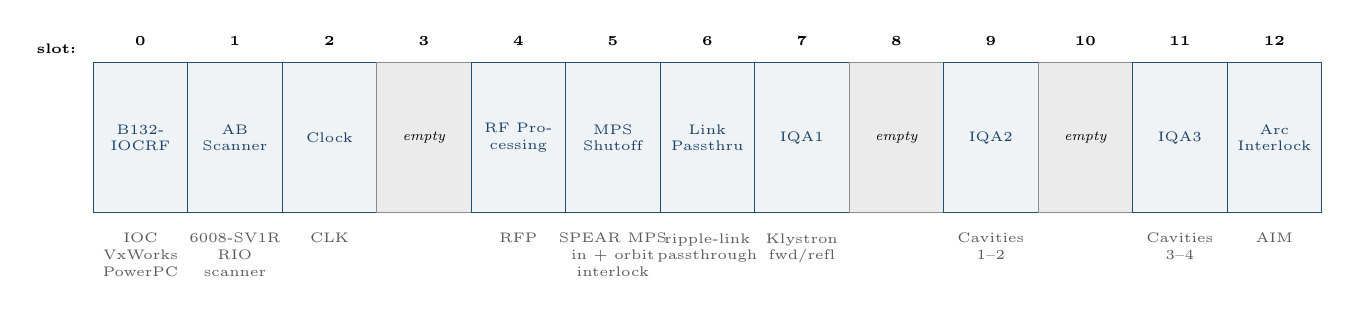
\begin{tikzpicture}[font=\tiny,x=1mm,y=1mm,every node/.style={outer sep=0pt}]
\def\w{12}   % slot pitch
\def\h{19}   % slot height

% slot/label/function/empty-flag
\foreach \i/\name/\fn/\e in {%
  0/{B132-\\IOCRF}/{IOC\\VxWorks\\PowerPC}/0,
  1/{AB\\Scanner}/{6008-SV1R\\RIO\\scanner}/0,
  2/{Clock}/{CLK}/0,
  3/{}/{}/1,
  4/{RF Pro-\\cessing}/{RFP}/0,
  5/{MPS\\Shutoff}/{SPEAR MPS\\in + orbit\\interlock}/0,
  6/{Link\\Passthru}/{ripple-link\\passthrough}/0,
  7/{IQA1}/{Klystron\\fwd/refl}/0,
  8/{}/{}/1,
  9/{IQA2}/{Cavities\\1--2}/0,
  10/{}/{}/1,
  11/{IQA3}/{Cavities\\3--4}/0,
  12/{Arc\\Interlock}/{AIM}/0}
{
  \ifnum\e=1
    \node[draw=black!45,fill=black!8,minimum width=\w mm,minimum height=\h mm,
          inner sep=1pt,align=center,font=\tiny\itshape,anchor=north west]
      at ({\i*\w},0) {empty};
  \else
    \node[draw=cCtrl,fill=cCtrl!7,minimum width=\w mm,minimum height=\h mm,
          inner sep=1pt,align=center,font=\tiny,text=cCtrl!85!black,
          anchor=north west] at ({\i*\w},0) {\name};
  \fi
  % slot number above
  \node[font=\tiny\bfseries,anchor=south] at ({\i*\w+\w/2},1) {\i};
  % function below
  \node[font=\tiny,align=center,anchor=north,text=black!65]
    at ({\i*\w+\w/2},{-\h-1.5}) {\fn};
}
\node[font=\tiny\bfseries,anchor=east] at (-1,1.8) {slot:};
\end{tikzpicture}
\end{fitpicture}
\caption{VXI crate slot map.  Elma 13-slot chassis,
  label B132-101-11-24.  Slots 3, 8 and 10 are empty: the gap-voltage
  feed-forward module and the two comb-filter modules that PEP-II carries are
  not required by SPEAR3.}\label{fig:vxi-crate}
\end{figure}

\begin{longtable}[]{@{}P{\dimexpr 0.0697\linewidth-1.500\tabcolsep\relax}P{\dimexpr 0.2190\linewidth-1.500\tabcolsep\relax}P{\dimexpr 0.5612\linewidth-1.500\tabcolsep\relax}P{\dimexpr 0.1502\linewidth-1.500\tabcolsep\relax}@{}}
\toprule\noalign{}
Slot & Module & Function & SPEAR3 Status \\
\midrule\noalign{}
\endhead
\bottomrule\noalign{}
\endlastfoot
0 & B132-IOCRF (Slot 0 μProcessor) & VXI bus controller, EPICS IOC host (VxWorks RTOS, Kinetics Systems) & \textbf{Active} \\
1 & AB Scanner & Allen-Bradley 6008-SV1R Remote I/O scanner (PLC interface) & \textbf{Active} \\
2 & CLK/RF Distribution & Master clock, LO generation (471.187 MHz = RF × 92/93), RF reference fanout (+14.0 dBm); CLK40/20/10 timing signals; TSYNC synchronization pulse & \textbf{Active} \\
3 & \emph{(empty)} & GVF slot from PEP-II --- not installed in SPEAR3 & \textbf{Not installed} \\
4 & RFP (RF Processor) & Central feedback processing --- IQ demod, vector sum, direct loop, baseband modulator & \textbf{Active} \\
5 & MPS Shutoff & CF2 slot from PEP-II, repurposed for MPS Shutoff in SPEAR3 & \textbf{Active} \\
6 & Link Passthru & RF amplifier Link passthrough module & \textbf{Active} \\
7 & IQA-1 & Klystron, circulator, drive, reference and WG01 load signals; ripple-link source & \textbf{Active} \\
8 & \emph{(empty)} & --- & --- \\
9 & IQA-2 & Cavity 1--2 forward, reflected and probe signals; WG02 load & \textbf{Active} \\
10 & \emph{(empty)} & --- & --- \\
11 & IQA-3 & Cavity 3--4 forward, reflected and probe signals; WG03 load & \textbf{Active} \\
12 & ARC/Interlock Module (AIM) & Arc detection, interlock management, fault history & \textbf{Active} \\
\end{longtable}

Slots 3, 8 and 10 are empty. The gap voltage feed-forward (GVF) module and the two comb-filter modules that PEP-II carries --- in its own slots 3, 5 and 6 --- are not required by SPEAR3, which instead uses slots 5 and 6 for the MPS shutoff and link passthrough functions \R{53}.

\subsection{CLK (Clock and RF Reference Distribution) Module}

The Clock module in VXI slot 2 is the master timing and RF reference source for the entire LLRF system, and is described first because every other module runs from its outputs. It was originally designed for PEP-II and modified for SPEAR3 frequencies.

\subsubsection{System Timing Parameters}\label{sec:timing-parameters}

\textbf{The SPEAR3 and PEP-II clocks use different division ratios}, so each column carries its own multiplier.

\begin{longtable}[]{@{}lll@{}}
\toprule\noalign{}
Parameter & SPEAR3 & PEP-II \\
\midrule\noalign{}
\endhead
\bottomrule\noalign{}
\endlastfoot
Storage Ring RF & 476.309 MHz & 476.000 MHz \\
RF Tuning Range & ±200 ppm & ±100 ppm \\
Ring Circumference & 234.126 m & 2199.33 m \\
Number of RF Buckets (h) & 372 & 3492 \\
Fiducial Rate $(f_\text{RF}/h)$ & 1.28040 MHz & 136.312 kHz \\
LO Frequency & 471.1874 MHz (RF × 92/93) & 471.0928 MHz (RF × 96/97) \\
CLK40 & 40.9728 MHz (32 × fiducial) & 39.2579 MHz (288 × fiducial) \\
CLK20 & 20.4864 MHz (16 × fiducial) & 19.6289 MHz (144 × fiducial) \\
CLK10 & 10.2432 MHz (8 × fiducial) & 9.8145 MHz (72 × fiducial) \\
PLL40 Ref Clock & 5.1216 MHz (RF/93) & 4.9072 MHz (RF/97) \\
\textbf{IF} $(= f_\text{RF} - f_\text{LO})$ & \textbf{5.1216 MHz} $(f_\text{RF}/93)$ & \textbf{4.9072 MHz} $(f_\text{RF}/97)$ \\
\end{longtable}

\begin{keynote}
\textbf{Design values}: The stated ±200 ppm RF tuning range is approximately ±95 kHz \R{53}.
\end{keynote}

\subsubsection{Clock Module Signals (Top-Level I/O)}

\Cref{fig:clock-io} shows the module's external connections; the signals are described below.

\begin{figure}[tbp]\centering
\begin{fitpicture}% !TeX root = ../L_legacy_system_architecture.tex
% VXI clock module: top-level inputs and outputs.
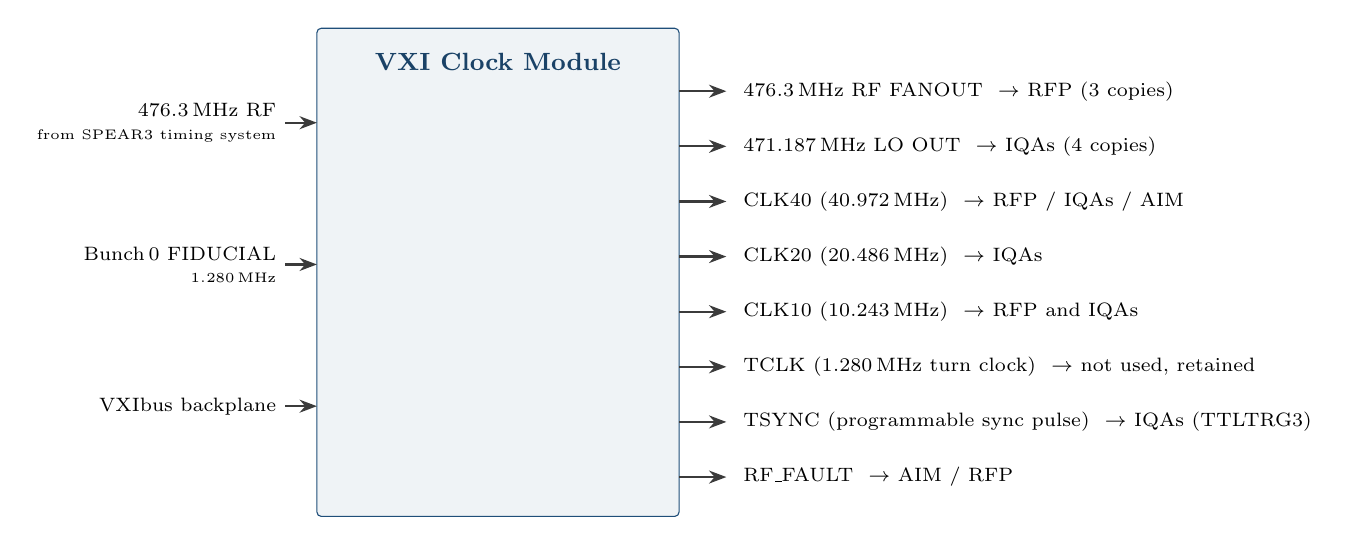
\begin{tikzpicture}[font=\scriptsize,x=1mm,y=1mm,every node/.style={outer sep=0pt}]
\node[ctrl,minimum width=46mm,minimum height=62mm,anchor=north west] (clk) at (52,0) {};
\node[font=\small\bfseries,text=cCtrl!85!black,anchor=north] at (75,-2) {VXI Clock Module};

% ---- inputs -------------------------------------------------------------
\node[anchor=east,align=right,font=\scriptsize] (in1) at (48,-12)
  {\qty{476.3}{\mega\hertz} RF\\{\tiny from SPEAR3 timing system}};
\node[anchor=east,align=right,font=\scriptsize] (in2) at (48,-30)
  {Bunch\,0 FIDUCIAL\\{\tiny \qty{1.280}{\mega\hertz}}};
\node[anchor=east,align=right,font=\scriptsize] (in3) at (48,-48)
  {VXIbus backplane};
\foreach \n/\y in {in1/-12,in2/-30,in3/-48}{\draw[sig] (\n.east) -- (52,\y);}

% ---- outputs ------------------------------------------------------------
\foreach \y/\txt in {%
  -8/{\qty{476.3}{\mega\hertz} RF FANOUT \ $\rightarrow$ RFP (3 copies)},
  -15/{\qty{471.187}{\mega\hertz} LO OUT \ $\rightarrow$ IQAs (4 copies)},
  -22/{CLK40 (\qty{40.972}{\mega\hertz}) \ $\rightarrow$ RFP / IQAs / AIM},
  -29/{CLK20 (\qty{20.486}{\mega\hertz}) \ $\rightarrow$ IQAs},
  -36/{CLK10 (\qty{10.243}{\mega\hertz}) \ $\rightarrow$ RFP and IQAs},
  -43/{TCLK (\qty{1.280}{\mega\hertz} turn clock) \ $\rightarrow$ not used, retained},
  -50/{TSYNC (programmable sync pulse) \ $\rightarrow$ IQAs (TTLTRG3)},
  -57/{RF\_FAULT \ $\rightarrow$ AIM / RFP}}
{
  \draw[sig] (98,\y) -- (104,\y);
  \node[anchor=west,font=\scriptsize] at (105,\y) {\txt};
}
\end{tikzpicture}
\end{fitpicture}
\caption{Clock module top-level inputs and outputs.}\label{fig:clock-io}
\end{figure}

\textbf{Signal descriptions}:

\begin{itemize}
\tightlist
\item
  \textbf{476.3 MHz RF FANOUT} --- Input from SPEAR3 timing system (minimum +9.0 dBm required); amplified to +14.0 dBm and fanned out to RFP and other modules; PKZ impedance-controlled connectors
\item
  \textbf{471.187 MHz LO} --- Phase-locked local oscillator ($= f_\text{RF} \times 92/93$); 4 copies at +14.0 dBm on front-panel PKZ connectors distributed to all three IQA modules for downconversion to 5.122 MHz IF
\item
  \textbf{CLK40} --- 40.972 MHz system clock; output on VXIbus backplane ECLTRG0 (bussed to all modules via P2); runs RFP and IQA digital logic; a delay vernier adjusts backplane timing skew
\item
  \textbf{CLK20} --- 20.486 MHz; output on ECLTRG1; drives IQA ADC quadrature sampling
\item
  \textbf{CLK10} --- 10.243 MHz; output on TTLTRG0 to RFP/IQA logic; also the reference for PLL471. The AIM uses CLK40
\item
  \textbf{TCLK} --- 1.280 MHz turn clock (50\% duty cycle); generated by ÷372 ECL counter locked to fiducial; output on TTLTRG1; not used by any SPEAR3 module (GAP module absent) but retained for diagnostics
\item
  \textbf{TSYNC} --- Programmable synchronization pulse derived from fiducial; width and delay are software-controlled via VXI registers; used by IQA and other modules to synchronize internal state machines; output on TTLTRG3
\item
  \textbf{RF\_FAULT} --- Open-collector backplane fault line; asserted by clock when RF input is lost or PLL loses lock; monitored by AIM and RFP
\end{itemize}

\subsubsection{Clock Module Architecture}

\Cref{fig:clock-arch} traces the two phase-locked loops and the divider chains that produce the signals listed above.Both PLLs and the RF input/fanout circuitry are housed in an temperature stabilized enclosure on the PCB to minimize phase noise, jitter, and frequency drift.

\begin{figure}[tbp]\centering
\begin{fitpicture}% !TeX root = ../L_legacy_system_architecture.tex
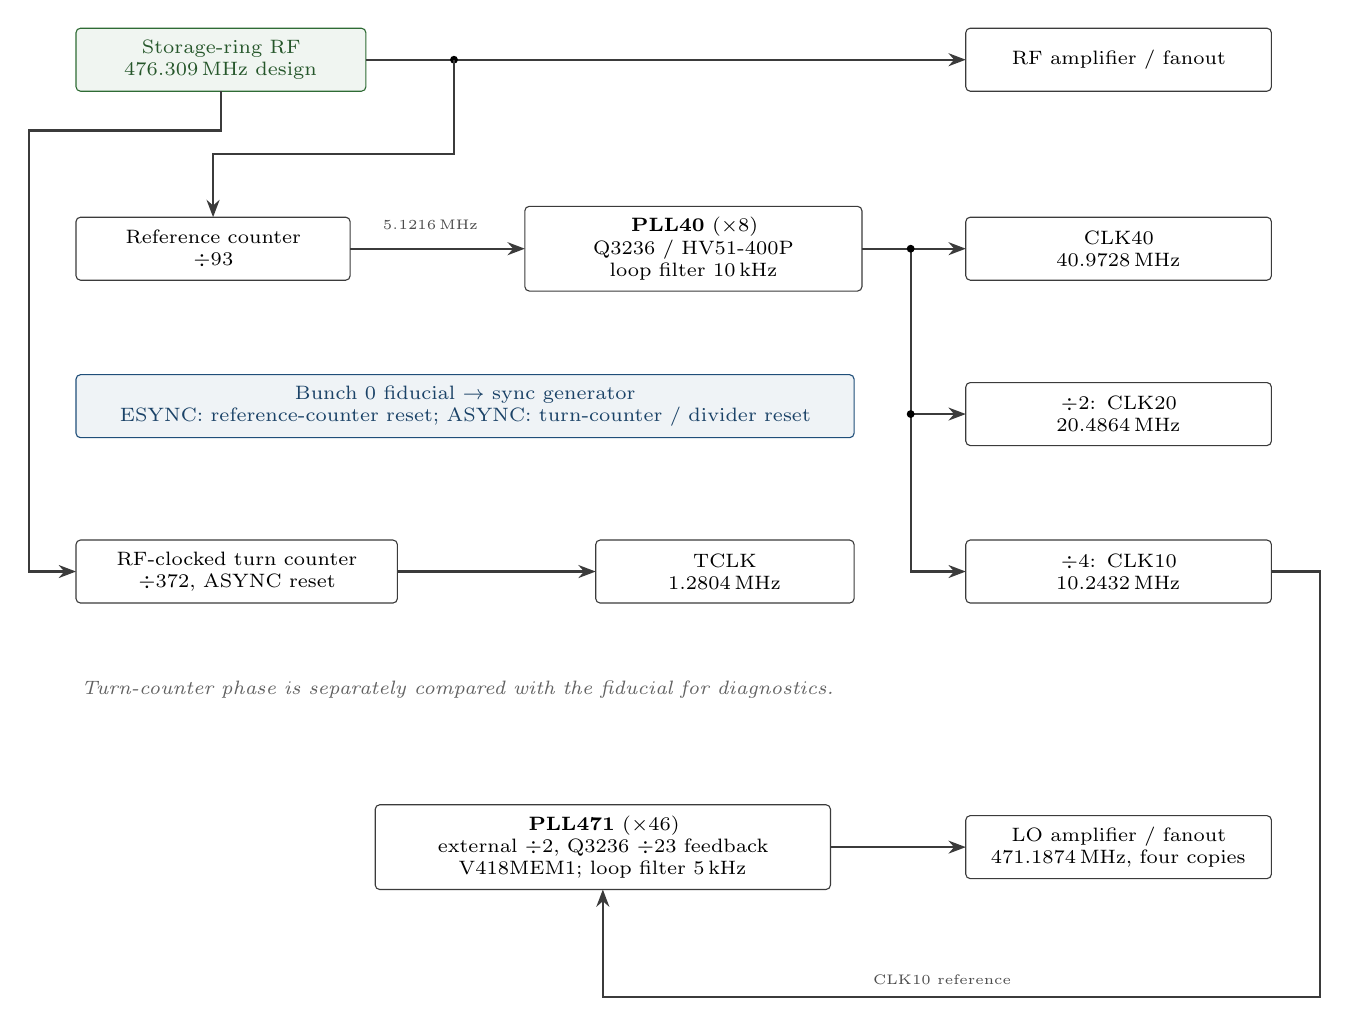
\begin{tikzpicture}[font=\scriptsize,x=1mm,y=1mm,every node/.style={outer sep=0pt}]
\node[rf,text width=34mm,anchor=west] (rfin) at (6,0)
  {Storage-ring RF\\\qty{476.309}{\mega\hertz} design};
\node[blk,text width=36mm,anchor=west] (fanout) at (119,0)
  {RF amplifier / fanout};
\draw[sig] (rfin.east) -- (fanout.west);
\fill (54,0) circle (0.5mm);

\node[blk,text width=32mm,anchor=west] (pre) at (6,-24)
  {Reference counter\\$\div93$};
\node[blk,text width=40mm,anchor=west] (pll40) at (63,-24)
  {\textbf{PLL40} ($\times8$)\\Q3236 / HV51-400P\\loop filter \qty{10}{\kilo\hertz}};
\draw[sig] (54,0) -- (54,-12) -| (pre.north);
\draw[sig] (pre.east) -- (pll40.west);
\node[tag,anchor=south] at (51,-22) {\qty{5.1216}{\mega\hertz}};

\node[blk,text width=36mm,anchor=west] (clk40) at (119,-24)
  {CLK40\\\qty{40.9728}{\mega\hertz}};
\node[blk,text width=36mm,anchor=west] (clk20) at (119,-45)
  {$\div2$: CLK20\\\qty{20.4864}{\mega\hertz}};
\node[blk,text width=36mm,anchor=west] (clk10) at (119,-65)
  {$\div4$: CLK10\\\qty{10.2432}{\mega\hertz}};
\draw[sig] (pll40.east) -- (clk40.west);
\draw[sig] (112,-24) -- (112,-45) -- (clk20.west);
\draw[sig] (112,-45) -- (112,-65) -- (clk10.west);
\fill (112,-24) circle (0.5mm);
\fill (112,-45) circle (0.5mm);

\node[ctrl,text width=96mm,anchor=west] at (6,-44)
  {Bunch 0 fiducial $\rightarrow$ sync generator\\
   ESYNC: reference-counter reset; ASYNC: turn-counter / divider reset};
\node[blk,text width=38mm,anchor=west] (turn) at (6,-65)
  {RF-clocked turn counter\\$\div372$, ASYNC reset};
\node[blk,text width=30mm,anchor=west] (tclk) at (72,-65)
  {TCLK\\\qty{1.2804}{\mega\hertz}};
\draw[sig] (rfin.south) -- ++(0,-5) -| (0,-65) -- (turn.west);
\draw[sig] (turn.east) -- (tclk.west);
\node[lbl,text width=96mm,anchor=west,align=left] at (6,-80)
  {Turn-counter phase is separately compared with the fiducial for diagnostics.};

\node[blk,text width=55mm,anchor=west] (pll471) at (44,-100)
  {\textbf{PLL471} ($\times46$)\\external $\div2$, Q3236 $\div23$ feedback\\
   V418MEM1; loop filter \qty{5}{\kilo\hertz}};
\node[blk,text width=36mm,anchor=west] (lo) at (119,-100)
  {LO amplifier / fanout\\\qty{471.1874}{\mega\hertz}, four copies};
\draw[sig] (clk10.east) -- (164,-65) -- (164,-119) -| (pll471.south);
\node[tag,anchor=south] at (116,-118) {CLK10 reference};
\draw[sig] (pll471.east) -- (lo.west);
\end{tikzpicture}
\end{fitpicture}
\caption{Functional clock chains from \R{53}. ESYNC and ASYNC synchronize counters/dividers; TCLK comes from the turn counter, with a separate fiducial-error comparison. Register, delay-vernier and fault circuitry are omitted.}\label{fig:clock-arch}
\end{figure}

\subsubsection{Changes Made to Adapt Clock for SPEAR3}

\begin{longtable}[]{@{}P{\dimexpr 0.2595\linewidth-1.000\tabcolsep\relax}P{\dimexpr 0.7405\linewidth-1.000\tabcolsep\relax}@{}}
\toprule\noalign{}
Item & Change for SPEAR3 \\
\midrule\noalign{}
\endhead
\bottomrule\noalign{}
\endlastfoot
PLL40 Ref prescaler & Division ratio changed to ÷93 \\
PLL40 VCXO & Changed to Connor-Winfield HV51-400P (40.972 MHz center, ±200 PPM, TTL output --- level-shift circuitry added to produce pseudo-ECL) \\
PLL471 feedback divider & Changed to ÷23 (external ÷2 + Q3236 internal ÷23; effective ratio 92/93 from 476.3 MHz) \\
Turn Counter & Division ratio changed to ÷372 \\
Configuration ID & DIP switch changed to indicate SPEAR3 model; IOC software verifies Config ID at boot \\
\end{longtable}


\subsection{RFP (RF Processor) Module --- Heart of the LLRF}

The RFP module is the central signal processing module in the VXI crate. It performs:

\textbf{Analog Signal Processing}:

\begin{itemize}
\tightlist
\item
  Direct analog quadrature demodulation of the cavity probe signals to baseband I/Q using the 476.3 MHz reference; the 5.122 MHz IF is used by the IQA modules, not this analog direct-loop path \R{53}
\item
  Vector summing of 4 cavity I/Q signals
\item
  Direct loop error amplifier comparing vector sum against IQ reference
\item
  Lead and integral compensation networks for loop stability
\item
  Baseband modulator (4 × Gilbert-cell multipliers in 2×2 matrix for I→I, I→Q, Q→I, Q→Q correction)
\item
  IQ RF modulator (baseband → 476 MHz upconversion for klystron drive)
\end{itemize}

\textbf{Digital Control Interface}:

\begin{itemize}
\tightlist
\item
  Octal DACs (12-bit, ±2048 counts) for: tune mode IQ setpoints, operate mode IQ offsets, klystron modulator matrix coefficients, ripple loop coefficients
\item
  Mode control: TUNE / OPERATE switching
\item
  RF switch: enable/disable RF output to klystron
\item
  Built-in history buffer (circular buffer, freeze on fault for post-mortem analysis)
\item
  Network analyzer and arbitrary waveform generator for loop-response measurements \R{53}
\end{itemize}

\textbf{Key PVs} (from \texttt{rf\_dac\_loop\_pvs.h,v}, \texttt{rf\_states.st,v}, and \texttt{rfp.db}):

\begin{center}\small
\begin{tabular}{@{}>{\ttfamily}l l@{}}
\toprule
\normalfont Process variable & Meaning \\
\midrule
\{STN\}:STN:TUNE:IQ.A & Tune mode IQ setpoint magnitude (counts) \\
\{STN\}:STN:TUNE:CTRL & Tune loop control \\
\{STN\}:STNDIRECT:LOOP:PHASE & Direct loop phase setpoint \\
\{STN\}:STNDIRECT:LOOP:COUNTS & Direct loop amplitude setpoint (counts) \\
\{STN\}:STN:RFP:RFENABLE & RF output enable/disable (from rf\_states.st) \\
\{STN\}:STN:RFP:RUNMODE & TUNE/OPERATE mode select (from rfp.db) \\
\{STN\}:STN:RFP:MODU.DLE & Direct loop enable (RFP module register) \\
\bottomrule
\end{tabular}
\end{center}


\subsection{IQA (IQ/Amplitude Detector) Modules}\label{sec:iqa-map}

Three IQA modules measure RF signals by downconversion and quadrature sampling \R{53}, producing:

\begin{itemize}
\tightlist
\item
  $I$ component (in-phase), $Q$ component (quadrature)
\item
  Amplitude $A = \sqrt{I^{2} + Q^{2}}$
\item
  Phase $\phi = \operatorname{atan2}(Q,I)$, retaining quadrant information
\end{itemize}

\textbf{Channel allocation}: The four-cavity station instantiates both IQA substitution files in \R{76}. Their zero-based \texttt{CH} indices give the following complete logical map; the parenthesized numbers are the corresponding one-based inputs.

\begin{longtable}[]{@{}Q{\dimexpr 0.12\linewidth-1.5\tabcolsep\relax}Q{\dimexpr 0.32\linewidth-1.5\tabcolsep\relax}Q{\dimexpr 0.28\linewidth-1.5\tabcolsep\relax}Q{\dimexpr 0.28\linewidth-1.5\tabcolsep\relax}@{}}
\toprule
CH (input) & IQA-1, slot 7 & IQA-2, slot 9 & IQA-3, slot 11 \\
\midrule
\endhead
\bottomrule
\endlastfoot
0 (1) & Klystron output forward & Cavity 1 forward & Cavity 3 forward \\
1 (2) & Klystron output reflected & Cavity 1 reflected & Cavity 3 reflected \\
2 (3) & Circulator load forward & Cavity 2 forward & Cavity 4 forward \\
3 (4) & Circulator load reflected & Cavity 2 reflected & Cavity 4 reflected \\
4 (5) & Klystron drive forward & Cavity 1 probe & Cavity 3 probe \\
5 (6) & Station RF reference & Cavity 2 probe & Cavity 4 probe \\
6 (7) & WG01 load forward & WG02 load forward & WG03 load forward \\
7 (8) & WG01 load reflected & WG02 load reflected & WG03 load reflected \\
\end{longtable}

IQA-1 also sources the backplane ripple link to the RFP \R{53}. The logical map is source-verified; match physical connector labels and cable destinations to the installed station before cabling work for the upgrade LLRF9 system.\openitem{O5}

Each IQA muxes 8 RF input channels through a single ADC in round-robin fashion, downconverting from 476.3 MHz to the 5.1216 MHz IF (using the 471.187 MHz LO from the CLK module) and bandpass-filtering at the IF before quadrature sampling with the 20.486 MHz CLK20. The PEP-II variant of the module uses a different IF (4.9072 MHz) and therefore a different bandpass filter --- this filter change was one of the modifications required to adapt the IQA to SPEAR3 \R{53}. The 8 channels also have amplitude threshold comparators that assert \texttt{RF\_FAULT} on the VXIbus backplane if any channel exceeds its programmed limit. Each IQA contains circular history buffers that record I/Q data per channel and can be read out over VXI after a fault.


\subsection{ARC Interlock Module (AIM)}

The AIM module provides the interface between the VXI crate and the external interlock system:

\begin{itemize}
\tightlist
\item
  Beam abort force/reset interface
\item
  Filament control signals
\item
  HVPS permissive signals
\item
  Fault history buffers --- two independent systems:

  \begin{itemize}
  \tightlist
  \item
    \textbf{System A} (12-channel AIM support): hardware history controlled through the \texttt{HISBUF}, \texttt{ADCMUX} and \texttt{ADCCTL} interfaces. The source defines HVPS-only or HVPS-plus-arc acquisition and fault-triggered stopping. Installed version, channel map and acquisition setup require confirmation \R{60}.
  \item
    \textbf{System B}: The IOC's \texttt{rf\_statesFF} state set requests module history-file exports after the shutdown sequence. It configures up to 11 file families, including an AIM export; these are not 11 additional AIM ADC channels.
  \end{itemize}
\item
  Station fault word monitoring (AIM reads \texttt{FISTAT} A16 register from Fast IC)
\item
  Arc-threshold configuration through the AIM \texttt{TRIPLVL} registers. Thresholds, channel enables and the physical sensor map must be recorded together \R{53}, \R{60}.
\end{itemize}

\textbf{AIM \texttt{FICTRL} control register} (A16 offset \texttt{0x20}): Dusatko identifies six outgoing control signals routed through the ARC chassis and its isolated interfaces \R{53}. The original register definition also includes a forced-fault test bit and beam-abort reset bit \R{60}:

\begin{longtable}[]{@{}Q{\dimexpr 0.23\linewidth-1.600\tabcolsep\relax}Q{\dimexpr 0.08\linewidth-1.600\tabcolsep\relax}Q{\dimexpr 0.25\linewidth-1.600\tabcolsep\relax}Q{\dimexpr 0.16\linewidth-1.600\tabcolsep\relax}Q{\dimexpr 0.28\linewidth-1.600\tabcolsep\relax}@{}}
\toprule\noalign{}
Signal & Bit & Symbol & Dusatko's six? & Ultimate destination \\
\midrule\noalign{}
\endhead
\bottomrule\noalign{}
\endlastfoot
\texttt{Solenoid\_On} & 0 & \texttt{AIM\_V\_SOLENOID} & Yes & Klystron solenoid power supply \\
\texttt{HVPS\_On} & 1 & \texttt{AIM\_V\_HVPS} & Yes & B514 HVPS SCR enable hardware \\
\texttt{Klys\_Filament\_On} & 2 & \texttt{AIM\_V\_FILAMENT} & Yes & Klystron filament heater supply \\
\texttt{Filament\_Timeout} & 3 & \texttt{AIM\_V\_FILTMOOVRD} & Yes & Fast IC filament-watchdog override \\
\texttt{Forced\_Fault} & 4 & \texttt{AIM\_V\_FRCDFLT} & \textbf{No --- test input} & Fast IC forced-fault test stimulus \\
\texttt{Fault\_Reset} & 5 & \texttt{AIM\_V\_FLTRESET} & Yes & Fast IC arc latch reset \\
\texttt{Beam\_Abort} & 6 & \texttt{AIM\_V\_FRCBMABT} & Yes & Facility beam-abort interface; installed endpoint requires confirmation \\
\texttt{Beam\_Abort\_Reset} & 7 & \texttt{AIM\_V\_RSTBMABT} & Yes & Facility beam-abort interface; resets the beam-abort latch \\
\end{longtable}

\textbf{\texttt{RF\_FAULT} backplane line}: Shared hardware fault line driven by the CLK, RFP, IQA, MPS interlock interface and AIM. The RFP uses it to inhibit klystron RF drive; the AIM monitors it for station fault handling \R{53}. This action does not depend on the Remote I/O scanner or SNL polling.

\textbf{Fault export}: The SNL exporter retrieves module histories; it is separate from the hardware mechanism that freezes those histories. File naming, trigger conditions and completeness checks are summarized in \cref{sec:fault-recording}.


\subsection{Feedback Loop Architecture}\label{sec:feedback-loops}

The legacy LLRF system implements multiple feedback loops, some inherited from PEP-II and some SPEAR3-specific:

\textbf{Active in SPEAR3}:

\begin{enumerate}
\def\labelenumi{\arabic{enumi}.}
\tightlist
\item
  \textbf{Direct RF Feedback Loop} --- Analog baseband feedback reduces the effective cavity impedance seen by the beam. The SPEAR3 system paper gives an approximately 800 kHz bandwidth and 15 dB impedance reduction \R{1}. 
\item
  \textbf{Tuner Loop} --- EPICS/SNL slow loop controlling the stepper motors to maintain cavity resonance. Implemented in \texttt{rf\_tuner\_loop.st,v} (\cref{sec:tuner-motion}).
\item
  \textbf{HVPS Voltage Regulation Loop} --- Regulates klystron cathode voltage via the PLC/analog-regulator SIG HI chain to the Enerpro SCR firing angle. Implemented across \texttt{rf\_hvps\_loop.st,v} (SNL) and PLC ladder logic (\cref{sec:analog-regulation}).
\item
  \textbf{DAC Control Loop} --- Manages drive power and gap voltage setpoints through the RFP octal DACs. Implemented in \texttt{rf\_dac\_loop.st,v}.
\item
  \textbf{Ripple Loop} --- RFP DSP1610 amplitude/phase regulation. Dusatko states that harmonic ripple removal is not implemented \R{53}; the 2004 paper describes adaptive cancellation \R{1}, and the 2021 test note measures harmonic rejection but does not isolate this loop's contribution \R{4}. 
\end{enumerate}

\textbf{NOT active in SPEAR3} (PEP-II only, module not installed):

\begin{itemize}
\tightlist
\item
  Comb (Narrowband) RF Feedback Loop --- PEP-II multi-bunch stabilization at revolution harmonics; the two CFM modules that implement it are absent from the SPEAR3 crate
\item
  Gap Voltage Feed-Forward (GVF/GAP) --- PEP-II gap-transient compensation with LFB interface; module absent. SPEAR3 instead obtains its station reference from a pair of RFP-resident DACs driven by a slow EPICS loop \R{53}. 
\end{itemize}

\subsection{Communication Architecture}\label{sec:communication}

The VXI slot-1 \textbf{Allen-Bradley 6008-SV1R scanner}, mounted through an HP E1407A adapter, controls one Remote I/O link \R{53}, \R{60}. Supervisory update rates depend on EPICS record scans and PLC data transfers; there is no single 1 Hz link rate. The direct RF loop and fast hardware interlocks bypass this serial link. \Cref{fig:comms-tree} shows the resulting hierarchy.

\begin{figure}[tbp]\centering
\begin{fitpicture}% !TeX root = ../L_legacy_system_architecture.tex
% Communication architecture: what hangs off the VXI IOC.
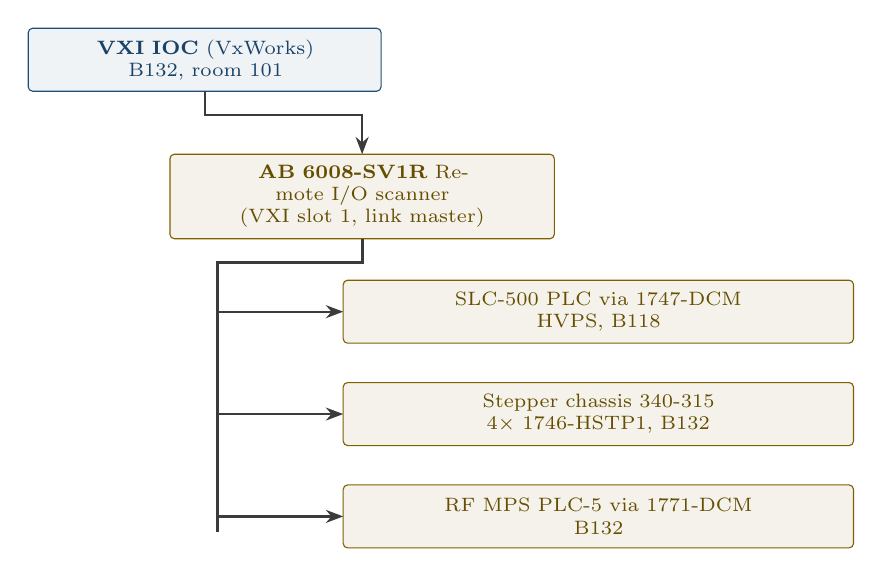
\begin{tikzpicture}[font=\scriptsize,x=1mm,y=1mm,every node/.style={outer sep=0pt}]
\node[ctrl,text width=42mm,anchor=north west] (ioc) at (0,0)
  {\textbf{VXI IOC} (VxWorks)\\ B132, room 101};

\node[plc,text width=46mm,anchor=north west] (scan) at (18,-16)
  {\textbf{AB 6008-SV1R} Remote I/O scanner\\ (VXI slot 1, link master)};

\node[plc,text width=62mm,anchor=north west] (r1) at (40,-32)
  { SLC-500 PLC via 1747-DCM\\ HVPS, B118};
\node[plc,text width=62mm,anchor=north west] (r2) at (40,-45)
  { Stepper chassis 340-315\\ $4\times$ 1746-HSTP1, B132};
\node[plc,text width=62mm,anchor=north west] (r3) at (40,-58)
  { RF MPS PLC-5 via 1771-DCM\\ B132};

% Orthogonal tree spines.  Stubs are drawn from (node.west -| rail) rather
% than a hardcoded y, so they stay horizontal whatever height a box turns out.
\coordinate (railB) at (24,0);
\draw[sig] (ioc.south) -- ++(0,-3) -| (scan.north);
\draw[bus] (scan.south) -- ++(0,-3) -| (24,-64);
\foreach \n in {r1,r2,r3}{\draw[sig] (\n.west -| railB) -- (\n.west);}
\end{tikzpicture}
\end{fitpicture}
\caption{Communication architecture below the VXI IOC.}\label{fig:comms-tree}
\end{figure}

\section{Klystron and Drive System}\label{sec:klystron-drive}

\subsection{Klystron}

The SPEAR3 klystron is a Marconi 476 MHz CW klystron located in Building B132. It is a single-beam tube with a non-full-power collector, meaning collector power must be actively managed to avoid thermal damage. Over the years, different tube models have been used, and the installed tube's exact specifications may vary.

\begin{longtable}[]{@{}ll@{}}
\toprule\noalign{}
Parameter & Value \\
\midrule\noalign{}
\endhead
\bottomrule\noalign{}
\endlastfoot
Frequency & \textasciitilde476.3 MHz (follows the ring size) \\
Manufacturer & Marconi \\
Power rating basis & 1.5 MW \\
Operating Output Power & \textasciitilde800 kW typical \\
Cathode Voltage & ≈ −72 to −75 kV typical; −90 kV maximum (HVPS rating) \\
Cathode Current & ≈ \qtyrange{19}{22}{\ampere} typical; 27 A maximum (HVPS rating) \\
Perveance & $I=K\lvert V\rvert^{3/2}$, $K\approx10^{-6}\,\mathrm{A\,V^{-3/2}}$ \R{56} \\
Drive Power & \textasciitilde29 W \\
Gain & \textasciitilde44.4 dB (800 kW / 29 W) \\
Collector type & Non-full-power (requires collector power protection) \\
\end{longtable}

\textbf{Collector Power Protection}: Because the klystron has a non-full-power collector, the collector dissipation (cathode power minus RF output power) must be monitored. In the legacy system, this is implemented through:

\begin{enumerate}
\def\labelenumi{\arabic{enumi}.}
\tightlist
\item
  The RF MPS computes a collector-power estimate from cathode power and measured RF output.
\item
  The Fast IC has a detected-klystron-power input (J16); this input alone is not a complete collector-power measurement.
\item
  Separately, processing mode in \texttt{rf\_hvps\_loop.st,v} reduces requested voltage for excessive \emph{forward RF power}, cavity voltage or vacuum. 
\end{enumerate}

\Cref{fig:marconi-klystron} shows the installed tube with its collector cooling and solenoid assembly. The heater is run from the separate filament control chassis of \cref{fig:klystron-filament-control-chassis}, which the AIM enables through \texttt{Klys\_Filament\_On}.

\photofig{marconi_klystron.png}{Marconi klystron in B132, with collector cooling and solenoid assembly.}{fig:marconi-klystron}

\photofig{klystron_filament_control_chassis.jpg}{Klystron filament control chassis --- manages the klystron heater/filament power and sequencing during startup and shutdown. The legacy chassis uses a motor-driven variac feeding a 10:1 step-down toroidal isolation transformer and a solid-state relay; it is enabled by the AIM \texttt{Klys\_Filament\_On} signal and its variac position is commanded through Allen-Bradley I/O \R{5}.}{fig:klystron-filament-control-chassis}


\subsection{Drive Amplifier}

The drive amplifier (KAW2051M12) boosts the LLRF drive signal to \textasciitilde29 W (44.6 dBm) at the station RF frequency (\textasciitilde476.3 MHz) to drive the klystron input.

The vendor rating is 125 W CW over 476 MHz ±5 MHz, with a 450--500 MHz frequency range, at least 55 dB gain and at most 50 ns group delay at 476 MHz \R{32}. \Cref{fig:rf-driver-amplifer} shows the spare unit held in B132.

\photofig{rf_driver_amplifer.jpg}{Spare RF drive amplifier (KAW2051M12) held in B132 --- amplifies the LLRF drive signal to \textasciitilde29 W (44.6 dBm) at \textasciitilde476.3 MHz to drive the klystron input}{fig:rf-driver-amplifer}


\section{Waveguide Distribution Network}\label{sec:waveguide}

\subsection{Network Topology}

The klystron output feeds a waveguide network that distributes RF power equally to the four cavities, as shown in \cref{fig:waveguide}.

\begin{figure}[tbp]\centering
\begin{fitpicture}% !TeX root = ../L_legacy_system_architecture.tex
% Waveguide distribution: klystron to four cavities through a circulator and
% three magic-tees. Reflected waves divide between source and difference
% ports according to their relative phases, not their powers alone.
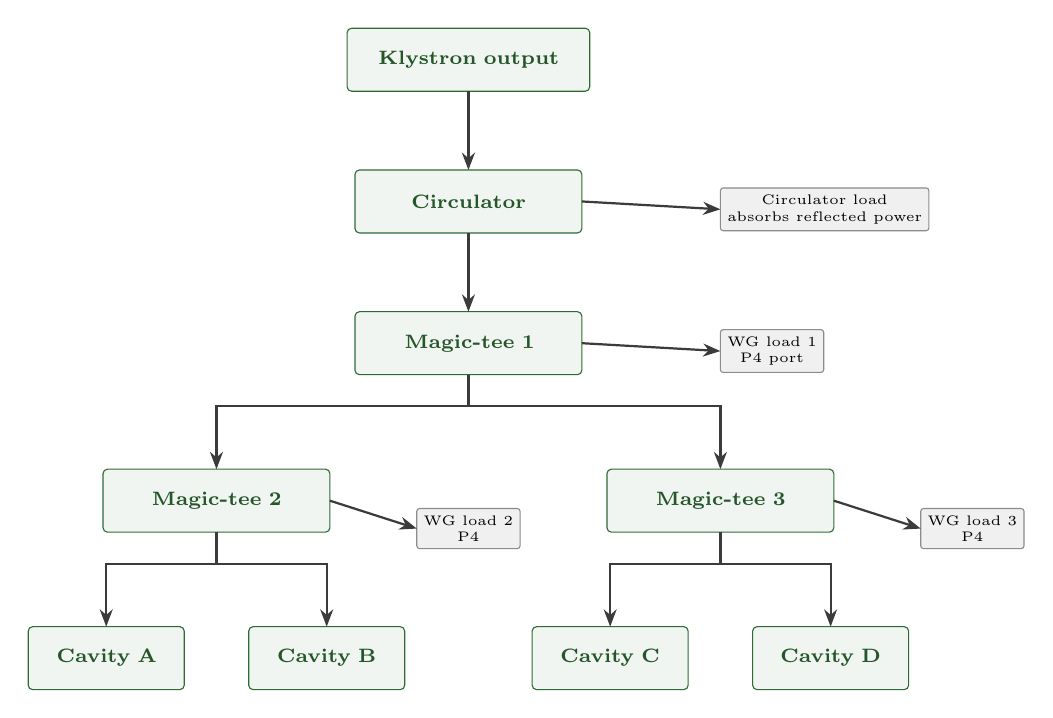
\begin{tikzpicture}[font=\scriptsize,x=1mm,y=1mm,every node/.style={outer sep=0pt}]
\tikzset{load/.style={draw=black!45,fill=black!6,rounded corners=1pt,
                      font=\tiny,align=center,inner sep=2.5pt}}

\node[rf,text width=28mm] (kly) at (60,0) {\textbf{Klystron output}};

\node[rf,text width=26mm,anchor=north] (circ) at (60,-14) {\textbf{Circulator}};
\draw[sig] (kly.south) -- (circ.north);
\node[load,anchor=west] (cl) at (92,-19) {Circulator load\\{\tiny absorbs reflected power}};
\draw[sig] (circ.east) -- (cl.west);

\node[rf,text width=26mm,anchor=north] (mt1) at (60,-32) {\textbf{Magic-tee 1}};
\draw[sig] (circ.south) -- (mt1.north);
\node[load,anchor=west] (l1) at (92,-37) {WG load 1\\{\tiny P4 port}};
\draw[sig] (mt1.east) -- (l1.west);

\node[rf,text width=26mm,anchor=north] (mt2) at (28,-52) {\textbf{Magic-tee 2}};
\node[rf,text width=26mm,anchor=north] (mt3) at (92,-52) {\textbf{Magic-tee 3}};
\draw[sig] (mt1.south) -- ++(0,-4) -| (mt2.north);
\draw[sig] (mt1.south) -- ++(0,-4) -| (mt3.north);

\node[load,anchor=north] (l2) at (60,-57) {WG load 2\\{\tiny P4}};
\node[load,anchor=north] (l3) at (124,-57) {WG load 3\\{\tiny P4}};
\draw[sig] (mt2.east) -- (l2.west);
\draw[sig] (mt3.east) -- (l3.west);

\foreach \x/\n/\lab in {14/ca/A, 42/cb/B, 78/cc/C, 106/cd/D}{
  \node[rf,text width=17mm,anchor=north] (\n) at (\x,-72) {\textbf{Cavity \lab}};
}
\draw[sig] (mt2.south) -- ++(0,-4) -| (ca.north);
\draw[sig] (mt2.south) -- ++(0,-4) -| (cb.north);
\draw[sig] (mt3.south) -- ++(0,-4) -| (cc.north);
\draw[sig] (mt3.south) -- ++(0,-4) -| (cd.north);
\end{tikzpicture}
\end{fitpicture}
\caption{Waveguide distribution network from klystron to cavities. Each
  magic-tee divides the incident power; return power divides between the
  source and load ports according to the relative phases of the returning
  waves.}\label{fig:waveguide}
\end{figure}

Each magic-tee splits incident power between two branches. Their return waves combine coherently at the source and difference-port load; equal reflected powers alone do not determine the destination. The waveguide electrical lengths set the relative phases \R{1}, \R{7}. The circulator diverts power returning toward the klystron to its own load. \Cref{fig:aft-circulator} shows that circulator and \cref{fig:magict-and-bellow-network-on-tunnel-roof} the magic-tee and bellows assembly on the tunnel roof.

\photofig{aft_circulator.png}{AFT circulator --- positioned between the klystron output and the magic-tee splitter network; routes reflected power from the load network away from the klystron to protect it from reflected energy}{fig:aft-circulator}

\photofig{magict_and_bellow_network_on_tunnel_roof.png}{Magic-tee power splitter and bellows network on the SPEAR3 tunnel roof --- the two-stage magic-tee arrangement divides RF power equally among all four cavities}{fig:magict-and-bellow-network-on-tunnel-roof}

\subsection{Monitored RF Signals}

The system monitors 24 RF signals at various points in the waveguide network. Key signals include:

\begin{itemize}
\tightlist
\item
  Klystron forward and reflected power (signals 1, 2)
\item
  Each cavity's forward power, reflected power, and probe signal (signals 9--14, 17--22)
\item
  Waveguide load powers (signals 7--8, 15--16, 23--24)
\item
  Station reference and klystron drive (signals 5, 6 --- 5 = klystron drive power, 6 = station reference power)
\item
  Circulator load forward and reflected power (signals 3, 4)
\end{itemize}

\Cref{fig:waveguide-network-from-klystron-to-cavity} shows the installed run from the klystron output into the tunnel. The circulator dump port and the magic-tee difference ports terminate in water-cooled loads (\cref{fig:water-load}) fed from the high-conductivity water station behind the booster (\cref{fig:hcw-station-behind-booster-forload}).

\smallfig{waveguide_network_from_klystron_to_cavity.png}{Waveguide distribution network routing RF power from the klystron output through the circulator, magic-tee splitters, and into the tunnel toward the four RF cavities}{fig:waveguide-network-from-klystron-to-cavity}

\photofig{water_load.png}{Water-cooled waveguide load --- absorbs circulator dump power and magic-tee difference-port reflected power; water cooling carries away dissipated RF energy. This load serves the magic-tee on the tunnel roof.}{fig:water-load}

\photofig{hcw_station_behind_booster_forload.png}{High-conductivity water (HCW) cooling station behind the booster --- supplies cooling water to the waveguide loads, absorbing reflected and dump power from the RF distribution network}{fig:hcw-station-behind-booster-forload}

\section{RF Cavities and Tuner Assemblies}\label{sec:cavities}

\subsection{Cavity Specifications}\label{sec:cavity-specs}

Four single-cell, HOM-damped copper cavities of the PEP-II HER design are installed in the ring \R{1}, \R{45}. Three waveguide ports couple HOM energy to loads. Each cavity provides:

\begin{itemize}
\tightlist
\item
  Accelerating gap voltage: \textasciitilde712 kV (operating)
\item
  Resonant frequency: tuned to the station RF frequency (\textasciitilde476.3 MHz), tuner-adjustable
\item
  3 HOM (Higher-Order Mode) loads per cavity for beam stability
\item
  Ceramic window for RF power transmission
\item
  Internal probe for field amplitude and phase monitoring
\end{itemize}

Each cavity has waveguide window viewports on either side of the ceramic window, providing mounting points for arc detection sensors.

\Cref{fig:pep-ii-bare-rf-cavity} shows a bare cavity body of this design and \cref{fig:rf-cavity-assembly} a complete assembly; the parts are named in \cref{fig:rf-cavity-assembly-with-names}. The tuner plunger enters from below (\cref{fig:movable-tunner-below-the-cavity}), and the three HOM loads terminate an E-plane mitre bend (\cref{fig:hom-load-at-e-mitre}), an H-plane mitre bend (\cref{fig:hom-load-at-h-mitre}) and a water-cooled plate (\cref{fig:hom-load-plate-water-cooled}). \Cref{fig:cavities-in-tunnel-outward-view} shows the installed row from the tuner side.

\photofig{pep_ii_bare_rf_cavity.png}{PEP-II bare single-cell RF cavity --- copper cavity body prior to installation of HOM dampers, tuner assembly, and waveguide couplers; the SPEAR3 cavities are of this same design}{fig:pep-ii-bare-rf-cavity}

\photofig{rf_cavity_assembly.png}{RF cavity assembly --- cavity body with waveguide coupler, HOM damper waveguide stubs, and tuner plunger installed}{fig:rf-cavity-assembly}

\smallfig{rf_cavity_assembly_with_names.png}{Labeled RF cavity assembly --- identifying the accelerating cell, input coupler, HOM damper ports, movable tuner plunger, probe port, and ceramic RF window}{fig:rf-cavity-assembly-with-names}

\photofig{movable_tunner_below_the_cavity.png}{Movable tuner plunger assembly mounted below an RF cavity --- the SLO-SYN stepper motor drives the plunger in/out to shift the cavity resonant frequency and minimize RF reflection under varying beam loading}{fig:movable-tunner-below-the-cavity}

\photofig{hom_load_at_e_mitre.png}{HOM (Higher-Order Mode) load at an E-plane mitre bend in the waveguide stub --- absorbs parasitic cavity modes that would otherwise cause beam instability}{fig:hom-load-at-e-mitre}

\photofig{hom_load_at_h_mitre.png}{HOM load at an H-plane mitre bend --- the three HOM loads per cavity (E-mitre, H-mitre, and plate) together damp all significant parasitic resonances above the fundamental accelerating mode}{fig:hom-load-at-h-mitre}

\photofig{hom_load_plate_water_cooled.png}{Water-cooled HOM load plate --- dissipates HOM power as heat, carried away by the high-conductivity water cooling system.}{fig:hom-load-plate-water-cooled}

\photofig{cavities_in_tunnel_outward_view.png}{Four RF cavities installed in the SPEAR3 storage ring tunnel (outward view, tuner side) --- showing the complete cavity row with waveguide distribution network and interconnecting bellows runs visible}{fig:cavities-in-tunnel-outward-view}

\subsection{Tuner Mechanical Assembly}

Each cavity has an individual stepper motor tuner that adjusts the cavity resonant frequency by varying the insertion depth of a mechanical plunger.

The 2023 inspection found that cavities A/B could challenge their lower bellows before the hardware stops acted, and that C's lower limit switch needed replacement. It also proposed a 12.5 mm upper software limit for A, whose upper switch actuated at 13.3 mm \R{36}.

\begin{keynote}
\textbf{Tuner travel --- checked September 2026.} J.~Sebek and R.~Lion checked the installed tuner mechanics. The hardware limit switches are presently set at approximately \textbf{±25 mm}, whereas the plunger actually moves only about \textbf{±4 mm} over a year of operation. The mechanical travel will therefore be restricted to \textbf{±10 mm}. That still covers the observed annual excursion with a wide margin, and a ±10 mm stroke does not stress the bellows.
\end{keynote}

\begin{longtable}[]{@{}P{\dimexpr 0.3189\linewidth-1.333\tabcolsep\relax}P{\dimexpr 0.4834\linewidth-1.333\tabcolsep\relax}P{\dimexpr 0.1977\linewidth-1.333\tabcolsep\relax}@{}}
\toprule\noalign{}
Component / parameter & Specification & Source \\
\midrule\noalign{}
\endhead
\bottomrule\noalign{}
\endlastfoot
Motor & Superior Electric SLO-SYN M093-FC11 (NEMA 34D) & \R{30} \\
Motor driver (in service) & Superior Electric SLO-SYN SS2000MD4-M PWM translator, one per motor (obsolete part) & \R{29} \\
Motor controller (in service) & Allen-Bradley 1746-HSTP1 stepper module, one per cavity, in chassis 340-315 & \R{78} \\
Motor controller (to be upgraded) & Galil DMC-4143 Rev 1.3h, 4-axis & \R{34}, \R{35} \\
Position feedback & Linear potentiometer on each tuner assembly (indication only --- not used to close the loop) & \R{36} \\
Step resolution & 0.003175 mm/step (1.27 mm/rev ÷ 400 steps/rev) & \texttt{rf\_cav.db,v} \texttt{DIST} \\
Slew setting & \texttt{VELO}=3 rev/s, equivalent to 3.81 mm/s; \texttt{ACCL}=0.5 s to velocity & Original record and device support \R{78} \\
Software travel limits & −29.5 mm (\texttt{DRVL}) to +18 mm (\texttt{DRVH}) & \texttt{rf\_cav.db,v} \\
Retry deadband & 0.015875 mm (exactly 5 steps) & \texttt{rf\_cav.db,v} \\
Loop rate & 2 Hz, 4 independent instances of \texttt{rf\_tuner\_loop.st,v} & \R{18} \\
\end{longtable}


\FloatBarrier\clearpage
\part{POWER SYSTEMS}


\section{High-Voltage Power Supply --- Power Section}\label{sec:hvps-power}

\subsection{Architecture Overview}

The HVPS is a 12-pulse thyristor phase-controlled rectifier based on the PEP-II design (SLAC, 1997) \R{6}. It delivers negative-polarity DC high voltage to the klystron cathode. The power section is located in Building B514; the control system is in Building B118.

Two complete HVPS units exist: \textbf{SPEAR1} and \textbf{SPEAR2}. Both are maintained in operating condition and connect to the klystron through a switch-over tank. At any time \textbf{one unit is energized and the other is completely switched off} --- this is not a warm-standby arrangement. The roles are exchanged at the two scheduled accelerator downs each year (April and August), which equalizes run-time and gives maintenance access to the off-duty unit. Either SPEAR1 or SPEAR2 may be the active unit.

\subsection{Power Conversion Chain}

\Cref{fig:hvps-chain} traces the conversion from the 12.47 kV substation feed to the klystron cathode.

\begin{figure}[tbp]\centering
\begin{fitpicture}% !TeX root = ../L_legacy_system_architecture.tex
% HVPS power conversion chain, substation to klystron cathode.
% Stage boxes on the left, parameters on the right.
% Written out node by node rather than with \foreach: the parameter text
% contains commas, which \foreach would treat as list separators.
\begin{tikzpicture}[font=\scriptsize,x=1mm,y=1mm,every node/.style={outer sep=0pt}]
\def\bx{46}
\newcommand{\stage}[4]{%   #1 name  #2 y  #3 title  #4 parameters
  \node[pwr,text width=54mm,anchor=north] (#1) at (\bx,#2) {\textbf{#3}};
  \node[anchor=north west,text width=76mm,font=\tiny,text=black!68] at (78,#2-1) {#4};}

\node[anchor=north,align=center,font=\scriptsize\bfseries,text=cPwr!85!black]
  (src) at (\bx,0)
  {Substation 507, Breaker 160\\
   {\normalfont\qty{12.47}{\kilo\volt} RMS $3\varphi$ \qty{60}{\hertz}}};

\stage{s1}{-14}{SWITCHGEAR (contactor panel)}
  {Disconnect switch, primary fuses and vacuum contactor.
   Ross HQ3 contactor + HCA-1-A controller}

\stage{s2}{-32}{PHASE-SHIFT TRANSFORMER T0}
  {\qty{350}{\kilo\voltampere} nominal component specification; extended delta.
   Input \qty{12.47}{\kilo\volt}; two phase-shifted sets at $\pm15^\circ$,
   \qty{12.91}{\kilo\volt} RMS $\varphi$--$\varphi$}

\stage{s3}{-50}{RECTIFIER TRANSFORMERS T1 ($+15^\circ$), T2 ($-15^\circ$)}
  {Open wye, \qty{1.5}{\mega\voltampere} each.
   T1-S1 = T1-S2 = T2-S1 = \qty{21.0}{\kilo\volt} RMS;
   T2-S2 = \qty{10.5}{\kilo\volt} RMS}

\stage{s4}{-68}{12-PULSE SCR BRIDGES}
  {Two six-pulse bridges, star-point connected to the open-wye primary centres.
   12 stacks $\times$ 14 Powerex T8K7 = 168 thyristors.
   Phase-angle control $0^\circ$--$180^\circ$.  Enerpro FCOG6100 + FCOAUX60.
   Snubbers \qty{0.047}{\micro\farad} per thyristor,
   \qty{0.015}{\micro\farad} per stack}

\stage{s5}{-92}{PRIMARY FILTER INDUCTORS L1, L2}
  {\qty{0.3}{\henry}, \qty{85}{\ampere} full load, \qty{0.38}{\ohm} DC.
   \qty{1084}{\joule} stored energy each}

\stage{s6}{-108}{SECONDARY RECTIFIERS + FILTER, 4 SERIES STAGES}
  {One stage per transformer secondary.
   Stage DC $-26$, $-26$, $-26$, $-\qty{13}{\kilo\volt}$
   $\rightarrow -\qty{91}{\kilo\volt}$ total.
   Filter capacitance \qty{8}{\micro\farad} \emph{per stage}
   ($\approx\qty{2}{\micro\farad}$ net) via a \qty{105}{\percent} tap.
   Output divider $\approx 10\,000{:}1$}

\stage{s7}{-132}{CROWBAR PROTECTION}
  {4 SCR stacks in series (SCR13--16), 6 thyristors per stack.
   Bushings \qty{100}{\kilo\volt} DC, \qty{80}{\kilo\ampere} peak fault current.
   Fiber-optic trigger; conducts $\approx\qty{10}{\micro\second}$ after trigger}

\stage{s8}{-152}{CABLE TERMINATION INDUCTORS L1, L2 (Grounding Tank)}
  {``350 µH 40A''.  Limits cable discharge current into the klystron}

\draw[sig] (src.south) -- (s1.north);
\foreach \a/\b in {1/2,2/3,3/4,4/5,5/6,6/7,7/8}{\draw[sig] (s\a.south) -- (s\b.north);}

\node[anchor=north,align=center,font=\scriptsize\bfseries,text=cPwr!85!black]
  (out) at (\bx,-168)
  {HV DC to klystron cathode\\
   {\normalfont$\approx -72$ to $-\qty{75}{\kilo\volt}$,
    \qtyrange{19}{22}{\ampere} typical;
    $-\qty{90}{\kilo\volt}$ / \qty{27}{\ampere} rated}};
\draw[sig] (s8.south) -- (out.north);
\end{tikzpicture}
\end{fitpicture}
\caption{HVPS power conversion chain, substation to klystron cathode.}\label{fig:hvps-chain}
\end{figure}

\begin{keynote}
\textbf{Supply rating versus T0 rating.} NWL's schematic and the SPEAR2 nameplate rate the complete supply at \textbf{2750 kVA, 12.5 kV, 127 A RMS} \R{70}, \R{75}. The separate nominal rating of the extended-delta phase-shifting transformer T0 is \textbf{350 kVA} in \R{22}. This is consistent with the original paper's statement that the phase-shifter size is less than 15\% of the full-load MVA \R{6}; its winding rating is not the station through-power rating.
\end{keynote}

\Cref{fig:hvps-shematic} is the annotated PEP-II schematic from which the SPEAR3 supply derives. The main oil tank (\cref{fig:hvps2-mainoiltank}) holds the transformers, inductors, filter components and rectifier stacks, with the thyristor stacks in their own isolated tank (\cref{fig:scr-assembly-intank-hvps2}). \Cref{fig:hvps-cable-switch-tank-at-building514} shows the switch tank that selects which unit feeds the klystron. \Cref{fig:hvps2-switchgear-oiltank} shows the installation as a whole and \cref{fig:hvps2-nameplate} the NWL rating plate cited above; \cref{fig:hvps2-oiltank-top-view} shows the tank top opened for the 2026 inspection.

\widefig{hvps_shematic.jpg}{PEP-II Klystron Power Supply --- annotated circuit schematic showing the complete power conversion chain from the 12.5 kV 3-phase input through the disconnect/breaker, phase-shifting transformer (T0), thyristor-controlled rectifier bridges (40 kV, 80 A), filter inductors, secondary rectifier stages, 8 µF/30 kV filter capacitors, 500 Ω/1 kW filter resistors, 30 kV/30 A rectifiers, Crowbar, and Termination Tank to the Klystron (90 kV, 27 A). The intermediate DC levels labeled on the power stage outputs (−26 kV, −52 kV, −77 kV, −90 kV) are cumulative stage tap voltages. The SPEAR3 HVPS is directly derived from this PEP-II design}{fig:hvps-shematic}

\tallfig{hvps2_mainoiltank.png}{HVPS2 main oil tank at Building B514 --- this large oil-immersed enclosure houses the phase-shift transformer (T0), the two rectifier transformers (T1, T2), the two filter inductors, four filter capacitors with their eight resistors, and the main and filter diode rectifier stacks. The SCR phase controller and the SCR crowbar are mounted inside it in their own isolated oil tanks with oil-to-oil bushings, so either can be serviced without contaminating the main tank oil \R{6}. SPEAR1 is an identical installation}{fig:hvps2-mainoiltank}

\tallfig{scr_assembly_intank_hvps2.jpg}{Thyristor stack assemblies inside the HVPS2 phase tank, viewed into the side access opening with the cover removed --- showing columns of Powerex T8K7 SCR thyristor discs (flat black cylinders) paired on copper bus bar assemblies with gate driver signal wiring; this photo was taken with SPEAR2 drained and accessed during the April 2026 scheduled downtime; SPEAR1 contains identical hardware}{fig:scr-assembly-intank-hvps2}

\tallfig{hvps_cable_switch_tank_at_building514.jpg}{HVPS cable switch tank at Building B514 --- provides the switchover connection between the SPEAR1 and SPEAR2 HVPS units and the klystron HV cable; allows the active unit to be changed without disconnecting the klystron high-voltage cable}{fig:hvps-cable-switch-tank-at-building514}

\widefig{hvps2_switchgear_oiltank.jpg}{HVPS2 installation at Building B514 showing the large beige oil-filled power supply enclosures, "SPEAR 2" identification label, and "DANGER HIGH VOLTAGE" placard on the panel door; the cable trays, conduit runs, and grounding conductors are visible; a "DO NOT ENERGIZE" lock-and-tag notice is visible at left (SPEAR2 is the off-duty unit); SPEAR1 forms an identical installation on the right of SPEAR2}{fig:hvps2-switchgear-oiltank}

\tallfig{SPEAR2_HVPS_Plate.jpg}{NWL manufacturer's rating plate on the SPEAR2
  transformer tank, at the left-hand end of the installation above. It reads: \textbf{Model No.\ 39308},
  \textbf{2,750 kVA klystron power supply}, input \textbf{12.5 kV at 127 A AC,
  3-phase, 60 Hz}, output \textbf{$-$90 kV DC at 27 A DC}, \qty{55}{\celsius} rise, Class OA,
  7.5\% impedance, 95 kV BIL, 2,600 gallons of oil, 67,400 lb, dated Mar 1997. The plate also
  carries the winding and rectifier schematic with its cumulative DC stage taps,
  and cites NWL drawings D36941 (physical outline) and D36943 (electrical
  schematic). SPEAR1 carries an identical
  plate}{fig:hvps2-nameplate}

\widefig{hvps2_oiltank_top_view.jpg}{HVPS2 main oil tank being accessed from the top during the 2026 HVPS inspection --- revealing the internal copper bus bar assembly and SCR bridge structures below}{fig:hvps2-oiltank-top-view}

\subsection{Key Component Specifications}\label{sec:hvps-components}

\begin{longtable}[]{@{}P{\dimexpr 0.1375\linewidth-1.333\tabcolsep\relax}P{\dimexpr 0.6737\linewidth-1.333\tabcolsep\relax}P{\dimexpr 0.1888\linewidth-1.333\tabcolsep\relax}@{}}
\toprule\noalign{}
Component & Specification & Source \\
\midrule\noalign{}
\endhead
\bottomrule\noalign{}
\endlastfoot
Complete HVPS assembly & \textbf{2750 kVA input}, 12.5 kV at 127 A RMS, three-phase, 60 Hz; output $-90$ kV DC at 27 A DC & NWL schematic \R{70}; SPEAR2 nameplate \R{75} \\
Phase-shift transformer T0 & \textbf{350 kVA nominal component specification}; extended-delta phase shifter producing two three-phase sets at $\pm15^\circ$. Approximately 12.91 kV RMS line-to-line at the rectifier-transformer primaries for a 12.47 kV input & \R{22}; \R{6}; \R{56} \\
Nameplate construction data & \qty{55}{\celsius} rise, Class OA (oil-immersed, self-cooled), \textbf{7.5\% impedance}, \textbf{95 kV BIL}, 2,600 gallons of oil, 67,400 lb. NWL drawings: D36941 physical outline, D36943 electrical schematic & NWL rating plate \R{75} \\
Rectifier transformers T1, T2 & 1.5 MVA each, open wye primary / dual wye secondary & SD-730-790-01-C1 \R{9}; \R{22} \\
Transformer secondaries & T1-S1 = T1-S2 = T2-S1 = 21.0 kV RMS φ--φ; T2-S2 = 10.5 kV RMS & \R{56} \\
Series DC stage taps & −26 kV, −52 kV, −77 kV, −90 kV (cumulative, as labeled on the schematic) & SD-730-790-01-C1 \R{9} \\
SCR stacks (phase control) & 12 stacks × 14 Powerex T8K7 = 168 thyristors. The schematic labels the thyristor-controlled rectifier assembly "40KV 80A"; this is not an individual-device rating & \R{56}; SD-730-790-01-C1 \R{9} \\
Thyristor snubbers / sharing & 0.047 μF across each thyristor; 0.015 μF R-C snubber per stack; MOVs plus ≈ 20 MΩ sharing resistor per thyristor (≈ 280 MΩ per stack) & \R{56} \\
Filter inductors L1, L2 & 0.3 H, 85 A full load, 0.38 Ω DC resistance & \R{56}; labeled "FILTER INDUCTOR" on SD-730-790-01-C1 \R{9} \\
Secondary rectifiers & 4 six-pulse main bridges in series, "RECTIFIERS 30KV 30A"; 4 filter bridges, "FILTER RECTIFERS 30KV 3A AVG" & SD-730-790-01-C1 \R{9}; \R{22}\\
Filter capacitors & "CAPACITORS 8uFD 30KV" --- \textbf{8 μF per stage × 4 series stages} (≈ 2 μF net) & SD-730-790-01-C1 \R{9}; \R{56} \\
Filter series resistors & "FILTER RESISTORS 500 OHMS 1KW" --- 8 total, two per stage, in oil & SD-730-790-01-C1 \R{9}; \R{22} \\
Additional output capacitor & 0.22 μF across the HVPS output (not shown on the top-level schematic) & \R{56} \\
Crowbar SCRs (SCR13--16) & 4 stacks in series, 6 thyristors per stack with 5 MΩ sharing resistors. The schematic labels the crowbar assembly "CROWBAR 40KV 80A" (per-stack device rating); the oil-to-oil feed-through bushings are separately rated 100 kV DC with 80 kA peak fault current & SD-730-790-01-C1 \R{9}; \R{22}; \R{6}; \R{56} \\
Cable termination inductors & \textbf{350 µH, 40 A} as built --- labeled "350 µH 40A" on the Grounding Tank drawing, where they are designated \textbf{L1 and L2}. Each is shunted by a 25 kV / 100 A diode and a 30 nF / 37 kV capacitor. \emph{SLAC-PUB-7591 \R{6} describes "small 200 μH inductors in the termination tank" --- that is the 1997 design figure; the as-built value is 350 μH.} & SD-730-790-05-C1 \R{62}; \R{6} \\
Output voltage divider & \textbf{Two identical dividers}, each \textbf{five 20 MΩ resistors in series (100 MΩ) into two 1 MΩ resistors in parallel (500 kΩ)} --- R1--R7 and R11--R17 on WD-730-794-04-C0 \R{71}, in its "TRANSFORMER TANK WD-730-792-01" section. Each feeds a coaxial run (VOLTAGE 1 via J7, VOLTAGE 2 via J8) to TS-3 "VOLTAGE MONITORS" as DC-VOLTAGE \#1 and \#2. \textbf{The 500 kΩ bottom leg is loaded by the regulator board's ≈ 10.5 kΩ input}, which dominates it; the resulting end-to-end scale factor is \(R_\text{load}/R_\text{div} = 10^4/10^8 =\) \textbf{1 × 10⁻⁴, i.e. ≈ 10,000:1} (9.1 V at 91 kV) \R{72}. Independently confirmed by the PS Monitor Board output labeled "+ Voltage 10 kV/V" & WD-730-794-04-C0 \R{71}; \R{72}; SD-730-793-12-C3 \R{61} \\
Output HV cable & Mil-C-17/81-0001 (formerly RG-220), ≈ 101--103 pF/m; ≈ 10 m HVPS → transfer tank, \textless{} 50 m transfer tank → termination tank & \R{56} \\
Regulator card & PC-237-230 (SD-237-230-14-C1), "PEP II RF System --- Enerpro Voltage and Current Regulator Board" & \R{12} \\
\end{longtable}

\subsubsection{SCR Trigger and Monitor Electronics (SD-730-793 series)}

The \texttt{SD-730-793-xx} drawings are \textbf{printed-circuit-board schematics for the trigger, interlock and monitoring electronics}.

\begin{longtable}[]{@{}P{\dimexpr 0.1665\linewidth-1.333\tabcolsep\relax}P{\dimexpr 0.2229\linewidth-1.333\tabcolsep\relax}P{\dimexpr 0.6106\linewidth-1.333\tabcolsep\relax}@{}}
\toprule\noalign{}
Drawing & Title & Role \\
\midrule\noalign{}
\endhead
\bottomrule\noalign{}
\endlastfoot
\textbf{SD-730-793-03-C4} & 2MW Klystron PS 12 kV SCR Driver Board (M. Nguyen, 23 MAY 02) & Gate drive to the phase-control thyristor stacks. Opto-isolated 6N-139 input; CD4047B astable plus CD4528 monostables; MIC-4451 drivers into IXFH12N90 MOSFETs and a 60T/60T/60T pulse transformer. On-drawing timing diagram: \textbf{TP1 = 50 μs ± 5\%, TP2 = 16 μs ± 1 μs (adj. by R2), TP4--TP5 = 5 μs / 5 μs / 18 μs ± 5\%} \\
\textbf{SD-730-793-04-C2} & 2MW Klystron Power Supply SCR Crowbar Trigger Board (M. Nguyen, 10-JUN-02) & Crowbar gate drive. Same 6N-139 / CD4047B / CD4538 / MIC-4451 / IXFH12N90 / 60T pulse-transformer topology, but on a \textbf{millisecond} envelope: \textbf{TP1 = 50 ms (adj. by R1), TP2 = 5 ms, TP3 = 44 μs (adj. by R2), TP4--TP5 = 3 × 5 μs optical SCR trigger}. A second output, \textbf{J1 (SIP4) "Output Plug to Old Slave Trigger Bd"}, driven by MIC-4427s, fires the slave boards so all four crowbar stacks trigger together \\
\textbf{SD-730-793-07-C2} & SCR Control Driver --- \textbf{Right Side} Trigger Interconnect Bd & Carries \textbf{J1 BNC "TRANSFORMER ARC TRIGGER"} and \textbf{J2 HFBR-2412 "F.O SCR ENABLE"} receiver; drives ±A/±B/±C SCR trigger outputs; exchanges the COMMANDS bus (+12V PWR, 24V FAULT/ENABLE, FO SCR ENABLE, CB ENABLE, SLAVE CB TRIG, PLC FORCE CB, SLAVE CB OFF) with the left-side board \\
\textbf{SD-730-793-08-C1} & SCR Control Driver --- \textbf{Left Side} Trigger Interconnect Bd & Carries \textbf{J1 BNC "KLYSTRON ARC TRIGGER"}, \textbf{J2 HFBR-2412 "F.O KLYSTRON CROWBAR"} receiver and \textbf{J3 HFBR-1412 "F.O STATUS"} transmitter; MONITORING bus M1 (SCR ENABLE MON, CB TRIG MON, CB MONITOR, KLYS ARC MON, SCR MONITOR, KLYS CB MON) \\
\textbf{SD-730-793-12-C3} & 2MW Klystron PS Monitor Board & Conditions the HVPS voltage and current monitors; outputs \textbf{BNC1 "+ Voltage 10 kV/V"}, \textbf{BNC2 "+ Current 5A/V"}, and a \textbf{BNC3 "CROWBAR"} input; isolated ±15 V rails via two NMH2415S DC-DC converters \\
\textbf{SD-730-793-13-C1} & 2MW Klystron Power Supply Optical SCR Trigger Board & Generates the gate pulse train through a 60T/60T/60T pulse transformer; power connector P1 carries \textbf{+240 V, +120 V, GND, +5 V, AC OUT} --- matching the 240 V first pulse / 120 V subsequent pulses described in \cref{sec:hvps-control-power} \\
\end{longtable}

These three fiber-optic ports --- SCR ENABLE (right board), KLYSTRON CROWBAR (left board) and STATUS (left board) --- are the B118 ↔ B514 fiber set.

Boards \textbf{-03}, \textbf{-04} and \textbf{-13} share the same \textbf{4DB-P107-06} power connector with the same pinout (+240 V, +120 V, GND, +5 V, AC OUT ×2), confirming that the two-level 240 V / 120 V gate-drive scheme is used on all three.

\begin{keynote}
\textbf{SCR variants}: SD-730-793-04-C2 distinguishes optical and conventional SCR trigger configurations by R3/R37 values of 24.9 kΩ and 78.70 kΩ respectively. The 2004 SPEAR3 paper reports optical SCRs \R{1}; this does not identify every presently installed stack.
\end{keynote}

Confirm SCR type and matching trigger-board configuration before replacing a board.\openitem{O8}


\begin{keynote}
\textbf{Two generations of crowbar trigger board exist.} \texttt{sd7307940400.pdf} is \textbf{SD-730-794-04-C0}, "SCR Crowbar Trigger Board", R. Cassel 11/08/99 --- an earlier design using +15 V logic, a 6N-138 optocoupler, discrete IRFD9120/IRFD110 gate drivers and IXYTH12N90 switches, with R3/R4 = 147 kΩ. It was superseded by SD-730-793-04-C2 (2002), which uses +12 V logic, a 6N-139, MIC-4451 drivers and IXFH12N90 switches with R3 = 24.9 kΩ. The "Old Slave Trigger Bd" referred to on the 2002 sheet is most likely a board of this 1999 vintage. \textbf{Component values are not interchangeable between the two generations.}
\end{keynote}


\subsection{Monitoring Signals (B514 → B118)}\label{sec:hvps-monitoring-signals}

Four analog monitoring signals are sent from the HVPS power section to the B118 control room and are wired to a four-channel oscilloscope in the Hoffman Box area:

\begin{longtable}[]{@{}P{\dimexpr 0.2053\linewidth-1.333\tabcolsep\relax}P{\dimexpr 0.2899\linewidth-1.333\tabcolsep\relax}P{\dimexpr 0.5048\linewidth-1.333\tabcolsep\relax}@{}}
\toprule\noalign{}
Signal & Purpose & Sensor \\
\midrule\noalign{}
\endhead
\bottomrule\noalign{}
\endlastfoot
HVPS Output Voltage & DC voltage monitoring and regulation feedback & ≈10,000:1 resistive divider \\
HVPS Output Current & DC current monitoring & Danfysik UltraStab DC-CT in the Termination Tank; output goes to both Slot-9 \texttt{1746-NI4} Input 3 and the PS Monitor Board \R{25} \\
Inductor 2 Voltage & T2 firing circuit timing verification (sawtooth) & Inductor tap \\
Transformer 1 Phase Current & T1 firing circuit health monitoring & Transformer CT \\
\end{longtable}

Two further sensors in the Termination Tank feed protection rather than monitoring: a \textbf{3.333 mΩ (15 A = 50 mV) shunt} in the HV return cable, wired via TS-6 20/21 to BNC-12 as the klystron arc trigger; and a \textbf{Pearson CT-110} (10 A/V) wide-bandwidth current transformer whose coaxial output feeds J1 of the Left Side Trigger Interconnect Board (SD-730-793-08-C1) and initiates a crowbar trigger on a large enough transient \R{25}.


\subsection{Stored Energy and Discharge Times}

The following estimates summarize the circuit models in J. Sebek's hazards note \R{56}. Isolation, discharge and absence-of-voltage verification require the applicable approved procedure and qualified personnel. The models assume the identified discharge paths remain intact.

\begin{longtable}[]{@{}P{\dimexpr 0.3931\linewidth-1.600\tabcolsep\relax}P{\dimexpr 0.1698\linewidth-1.600\tabcolsep\relax}P{\dimexpr 0.1311\linewidth-1.600\tabcolsep\relax}P{\dimexpr 0.1311\linewidth-1.600\tabcolsep\relax}P{\dimexpr 0.1749\linewidth-1.600\tabcolsep\relax}@{}}
\toprule\noalign{}
Component & Value & Stored energy & Time constant & Estimated decay time \\
\midrule\noalign{}
\endhead
\bottomrule\noalign{}
\endlastfoot
Filter inductor (each of 2) & 0.3 H at 85 A & 1,084 J & \textless{} 0.1 s & \textless{} 0.1 s \\
Phase stack snubber capacitor & 0.015 μF at 18.26 kV & 2.5 J & 4.2 s & 24.8 s \\
Per-thyristor snubber capacitor & 0.047 μF & 40 mJ & 0.94 s & 3.1 s \\
Filter capacitors (normal shutdown) & ≈ 2 μF net & 8,788 J & \textless{} 1 s & \textless{} 1 s \\
Additional output capacitor & 0.22 μF & 911 J & \textless{} 1 s & \textless{} 1 s \\
Output cables & ≈ 0.006 μF & 25 J & \textless{} 1 s & \textless{} 1 s \\
\textbf{Total output capacitance (source removed, normal load)} & \textbf{≈ 2.23 μF} & \textbf{≈ 9,724 J} & \textbf{\textless{} 1 s} & \textbf{\textless{} 1 s} \\
Total output capacitance (source and klystron load removed) & ≈ 2.23 μF & ≈ 9,724 J & 20.9 s & 160 s \\
Filter capacitors (only filter-rectifier bleeders connected) & 8 μF per stage & 8,788 J total & 640 s & \textbf{4,890 s} \\
\end{longtable}

Capacitor times refer to decay below 50 V at the output, or below 12.5 V per series stage where that approximation is used. The inductor row describes current/energy decay, not a voltage clearance criterion.

\textbf{Normal turn-off.} The controller inhibits all phase-control stacks except B+ and B-, which provide a freewheel path for the primary-inductor current. The measured inductor voltage decays in about 10 ms. The source-free klystron-load model predicts capacitor decay below 50 V in about 250 ms, but an energized primary leaves approximately \textbf{1.3 kV} of rectified leakage at the output after firing is inhibited \R{56}. A normal RF shutdown is therefore not electrical isolation.

\textbf{Abnormal configurations.} The 81.5-minute estimate assumes the filter-rectifier bleeders remain connected. Further disconnection or component failure can remove that path entirely. No finite discharge time is established here for an isolated capacitor.

\subsection{Control Power and Trigger Pulses}\label{sec:hvps-control-power}

\begin{longtable}[]{@{}P{\dimexpr 0.2282\linewidth-1.000\tabcolsep\relax}P{\dimexpr 0.7718\linewidth-1.000\tabcolsep\relax}@{}}
\toprule\noalign{}
Item & Specification \\
\midrule\noalign{}
\endhead
\bottomrule\noalign{}
\endlastfoot
DC control power & 125 V DC from Substation 507, used by the local contactor controller in the switchgear; also feeds its local MPS for transformer tank overpressure, main tank oil temperature, and LCW flow through the oil cooling radiators \\
AC control power & Three phases of 208 V AC --- one for the contactor controller, one for the main-tank oil pump, one for the switchgear compartment light \\
Thyristor gate trigger pulses & Trains of 16 μs pulses in 15° bursts; first pulse 240 V, subsequent pulses 120 V. Similar amplitudes fire the crowbar thyristors \\
\end{longtable}


\section{HVPS Control System (B118)}\label{sec:hvps-control}

\subsection{Overview}

Each HVPS unit has \textbf{two} Hoffman NEMA enclosures of its own, standing side by side in Building B118. Both are called "the Hoffman box" in conversation --- indeed the door label on the smaller one also reads \textbf{"HOFFMANN BOX"} --- so this document keeps them apart by function:

\begin{itemize}
\tightlist
\item
  The \textbf{controller enclosure} --- the large cabinet, titled \textbf{TRIGGER ENCLOSURE} on its own master wiring diagram WD-730-790-02-C6 \R{63}. It holds the SLC-500 PLC, the analog regulation electronics, the Enerpro SCR firing boards, the power supplies, the terminal strips and the fiber-optic interfaces. Its door carries the unit identification label, a DANGER HIGH VOLTAGE placard, the lock-and-tag procedure form and the SLAC HV Switching Order. \Crefrange{sec:slc500-hardware}{sec:terminal-strips} describe its contents.
\item
  The \textbf{local control panel} --- the smaller enclosure beside it, which is the operator interface: a QuickPanel II touchscreen, four permit status lamps, ON and OFF pushbuttons, an EMERGENCY OFF mushroom and the PERMIT key switch. It appears on \R{63} as the \textbf{LOCAL CONTROL PANEL} block, where the mushroom is drawn as switch \textbf{S1} with \emph{two} normally-closed contacts (\cref{sec:emergency-off}).
\end{itemize}

SPEAR1 and SPEAR2 each have a complete pair; the off-duty unit's pair is de-energized along with its power section. \Cref{fig:hoffman-boxes} shows the two enclosures side by side --- SPEAR1 active in \cref{fig:hoffman-box-spear1} and SPEAR2 switched off in \cref{fig:hoffman-box-spear2}. \Cref{fig:hoffman-box-spear1-opened} shows the controller-enclosure interior and \cref{fig:hoffman-box-local-panel} the local control panel.

\begin{samepage}

\tallpairfig
  {hoffman_box_spear1.jpg}
  {SPEAR1 --- the active unit. The door carries the identification label, a
   DANGER HIGH VOLTAGE placard, the lock-and-tag procedure form and the SLAC
   HV Switching Order.}{fig:hoffman-box-spear1}
  {hoffman_box_spear2.jpg}
  {SPEAR2 --- identical hardware, switched off. The posted oscilloscope trace
   shows 12-pulse thyristor firing waveforms from HER B-2, circa 2007.}{fig:hoffman-box-spear2}
  {HVPS controller enclosures in Building B118. The two units are
   identical; one is energized and the other completely switched off, with the
   roles exchanged at each scheduled down.}{fig:hoffman-boxes}

\tallfig{hoffman_box_spear1_opened.jpg}{HVPS controller enclosure interior
  (SPEAR1) --- the SLC-500 PLC rack (center, a 10-slot chassis carrying the CPU
  and I/O modules in slots 0--9 with slot 4 empty, labeled "SPEAR 1 RFHVPS"),
  four blue KEPCO DC supplies --- \textbf{PS-1} 120 V/1 A, \textbf{PS-2}
  240 V/0.25 A, \textbf{PS-3} 5 V/20 A and \textbf{PS-4} 120 V/1 A, in that
  order on both the chassis labels and \R{63} --- the Enerpro FCOG6100
  SCR firing board (dark blue PCB, lower center), the analog regulation board
  (green PCB), and terminal strips TS-1 to TS-6 in the lower section; the BNC
  monitoring output panel is at lower right. On \R{63} the three rails arrive at
  every SCR gate-trigger module as \texttt{+100V} (red, PS-1 and PS-4),
  \texttt{+200V} (orange, PS-2) and \texttt{BIAS} (blue, PS-3), and rung 0068
  switches their 120 V AC feed; whether the 5 V rail is still loaded has not been
  checked.\openitem{O13}}{fig:hoffman-box-spear1-opened}

\tallfig{SPEAR1_hoffman_box_touchPanel_statusLEDs.jpg}{SPEAR1 \textbf{local
  control panel} labeled "SPEAR 1 HOFFMANN BOX". Across the top are the
  four permit status lamps \textbf{PPS PERMIT}, \textbf{EMERGENCY OFF},
  \textbf{KEY ENABLE} and \textbf{WAVEGUIDE PERMIT} --- LED1 to LED4 of the
  LOCAL CONTROL PANEL block on \R{63} --- all lit green here. Below them are the
  OFF and ON pushbuttons, the EMERGENCY OFF mushroom, and the \textbf{PERMIT}
  key switch, which must be turned from DISABLE to \textbf{ENABLE} before the
  HVPS can be switched on; the key contact drives SLC-500 slot 6 IB16 IN12,
  labeled "KEY ENABLE" on \R{63}. The QuickPanel II touchscreen is the local
  operator display, with a taped warning that only its lower-left corner may be
  touched to wake it, because a stray touch elsewhere can shut the RF HVPS off.
  SPEAR2 has an identical panel.}{fig:hoffman-box-local-panel}

\end{samepage}

\FloatBarrier

\subsection{SLC-500 PLC Hardware Configuration}\label{sec:slc500-hardware}

\begin{longtable}[]{@{}P{\dimexpr 0.0725\linewidth-1.333\tabcolsep\relax}P{\dimexpr 0.2229\linewidth-1.333\tabcolsep\relax}P{\dimexpr 0.7046\linewidth-1.333\tabcolsep\relax}@{}}
\toprule\noalign{}
Slot & Module & Function \\
\midrule\noalign{}
\endhead
\bottomrule\noalign{}
\endlastfoot
0 & SLC-500 CPU (AB-1747-L532) & Main processor \\
1 & 1747-DCM (DCM-FULL) & Remote I/O adapter --- presents the SLC-500 to the VXI 6008-SV1R scanner as RIO rack 1 \\
2 & 1746-IO8 & 8-point digital I/O. OUT3 (terminal 5) drives the Ross Grounding Switch coil (120 VAC); also 12 kV and 240 V control \\
3 & Thermocouple Module & 8-channel temperature sensing (4 channels actively scaled) \\
4 & (empty) & Unused slot \\
5 & 1746-OX8 & 8-point relay output. OUT1 = Contactor On/Off (TS-5 2); OUT2 = Contactor Enable → K4 coil (TS-5 4); also SCR enable, crowbar, fast inhibit \\
6 & 1746-IB16 & 16-point 24 V DC digital input --- interlock, oil-level, arc, permit and PPS status. Complete input map in \cref{sec:slot6-inputs} \\
7 & 1746-IV16 & 16-point 24 V DC digital input. IN0 = Blocking relay; IN1 = Overcurrent; IN2 = Contactor Closed/OK; IN3 = Contactor Ready; IN13 = Ross Ground Relay NO \\
8 & AB-1746-NIO4V & 4-channel analog I/O (voltage reference output, phase angle readback) \\
9 & AB-1746-NI4 & 4-channel analog input. IN3 = Danfysik DC-CT output (HVPS current); also AC current and voltage monitors \\
\end{longtable}

\subsubsection{Slot 6 --- 1746-IB16 digital input map}\label{sec:slot6-inputs}

WD-730-790-02-C6 \R{63} prints all sixteen input labels along the terminal block of the slot-6 module, numbered 0--15 with terminals 16 and 17 as DC COM. Seven of the sixteen are independently corroborated --- five by the PLC symbol database \R{27} and six by the PPS wiring trace \R{25}, overlapping on four --- and all seven agree position for position.

\begin{longtable}[]{@{}Q{\dimexpr 0.09\linewidth-1.500\tabcolsep\relax}Q{\dimexpr 0.32\linewidth-1.500\tabcolsep\relax}Q{\dimexpr 0.10\linewidth-1.500\tabcolsep\relax}Q{\dimexpr 0.49\linewidth-1.500\tabcolsep\relax}@{}}
\toprule\noalign{}
IN & Label as drawn & Wire & Cross-check and notes \\
\midrule\noalign{}
\endhead
\bottomrule\noalign{}
\endlastfoot
0 & SCR DISABLE & YEL & Drawing only \\
1 & CROWBAR TRIGGER MON & BLU & Drawing only \\
2 & CROWBAR MONITOR & GRAY & Drawing only \\
3 & KLYSTRON ARC MONITOR & BLK & Drawing only \\
4 & SCR MONITOR \# 1 & RED & Drawing only \\
5 & XFORMER ARC MONITOR & BLK & Drawing only \\
6 & SCR MONITOR \# 2 & RED & Drawing only \\
7 & KLYSTRON CB MON & BRN & \R{27} names this point \texttt{KLYSTRON\_CROWBAR} \\
8 & GRN TANK OIL OK & RED & \R{27} "GRN TANK OIL LEVEL"; \R{25} Grounding Tank oil level \\
9 & GRN SWITCH CLOSED & GRAY & \R{27} "Grounding Switch closed"; \R{25} manual grounding-switch auxiliary contact \\
10 & CROWBAR OIL LVL OK & VIOL & \R{27} "CROWBAR OIL LEVEL"; \R{25} crowbar tank oil level \\
11 & SCR OIL LEVEL OK & YEL & \R{27} "SCR OIL LEVEL"; \R{25} SCR phase tank oil level \\
12 & KEY ENABLE & ORG & The PERMIT key switch on the local control panel, which must be at ENABLE before the HVPS can be switched on \\
13 & EMERGENCY OFF & BLK & Contact \textbf{S1B} of the EMERGENCY OFF mushroom, via TS-8 terminal 2 (\cref{sec:emergency-off}) \\
14 & PPS \# 1 & GRN & PPS enable channel 1, GOB pin E; the same loop drives the PPS4 red status lamp and passes through mushroom contact \textbf{S1A} \R{25} \\
15 & PPS \# 2 & BLU & PPS enable channel 2, GOB pin G; the same wire drives the PPS3 red status lamp  \R{25} \\
16--17 & DC COM & --- & Module commons \\
\end{longtable}

\begin{keynote}
\textbf{What is not established}: \R{27} lists addresses \texttt{I:6/0}--\texttt{I:6/6} and \texttt{I:6/12}--\texttt{I:6/15} with their \textbf{symbol fields blank}, so their correspondence to ladder rungs and to EPICS PVs has not been traced. 
\end{keynote}

\subsection{Control Functions}

The PLC implements the following control functions in ladder logic:

\begin{enumerate}
\def\labelenumi{\arabic{enumi}.}
\tightlist
\item
  \textbf{Power-up/power-down sequencing} --- Orderly startup of contactors, SCR drives, and HVPS output
\item
  \textbf{Voltage reference generation} --- Converts the EPICS setpoint (via VXI → Remote I/O) into the analog reference for the regulator board
\item
  \textbf{SIG HI feedforward} --- Computes an approximate SIG HI value for the Enerpro board from the target voltage
\item
  \textbf{Safety interlock monitoring} --- Monitors oil levels, temperatures, PPS status, fiber optic signals
\item
  \textbf{Crowbar management} --- Arms/disarms crowbar protection, handles crowbar events
\item
  \textbf{Communication} --- Exchanges input and output data tables with the VXI IOC over the Remote I/O link 
\end{enumerate}

\textbf{Key PLC Registers}:

\begin{longtable}[]{@{}ll@{}}
\toprule\noalign{}
Register & Purpose \\
\midrule\noalign{}
\endhead
\bottomrule\noalign{}
\endlastfoot
N7:10 & Voltage reference output (to analog regulator) \\
N7:11 & Phase angle / SIG HI feedforward \\
N7:100--N7:107 & Thermocouple raw readings \\
N7:110--N7:113 & Scaled temperature values \\
I:1 / O:1 & Remote I/O data words (VXI interface) \\
\end{longtable}

\textbf{PPS-related ladder rungs} (from the original code review in \R{25}):

\begin{longtable}[]{@{}P{\dimexpr 0.0816\linewidth-1.000\tabcolsep\relax}P{\dimexpr 0.9184\linewidth-1.000\tabcolsep\relax}@{}}
\toprule\noalign{}
Rung & Function \\
\midrule\noalign{}
\endhead
\bottomrule\noalign{}
\endlastfoot
0002 & \texttt{ENABLE B3:0/6}, in series with system-ready, manual-ground-switch and remote-on conditions → Close Contactor \texttt{O:5/1}, the point \R{63} labels \textbf{CONT. ON/OFF}. The seal-in branch parallels only the momentary ON pulses, so \texttt{ENABLE} is a hard series permissive \\
0014 & \texttt{I:6/13} EMERGENCY OFF (examine-if-open) \textbf{in series with} PPS 1 → emergency-off latch, alarm and the \texttt{O:1/107} status bit \\
0015 & PPS 1 \textbf{in parallel with} PPS 2 → sets \texttt{B3:1} "PPS ON" \\
0016 & PPS 1 \textbf{in series with} PPS 2 (and other conditions) → energizes the Ross Grounding Switch relay coil \\
0017 & In series with Touch Panel Enable and Emergency Off Clear → OX8 OUT2. \emph{The rung is labeled "Crowbar On" in the PLC listing, but \R{25} concludes the label is wrong; \R{63} settles it by printing OX8 OUT2 as} \textbf{CONT. ENABLE} \\
0068 & PPS 2 in series with the touch-panel key enable → Bias Power (120 VAC to the Kepco supplies) \\
\end{longtable}


\subsection{The EMERGENCY OFF Mushroom}\label{sec:emergency-off}

On \R{63} the mushroom is switch \textbf{S1} of the LOCAL CONTROL PANEL block, and it carries \textbf{two} normally-closed contacts rather than one:

\begin{itemize}
\tightlist
\item
  \textbf{S1B} sits in the EMERGENCY OFF lamp loop and returns on TS-8 terminal 2 to slot-6 \texttt{IN13}.
\item
  \textbf{S1A} sits in the \emph{PPS PERMIT} lamp loop and returns on TS-8 terminal 1 to slot-6 \texttt{IN14}, the PPS~\#1 input. \R{25} traces the same loop point to point --- TS-8 1 to slot 6 IN 14 on green, then the PPS4 lamp anode, then white to the "Local Panel Emergency Off Key switch 1A".
\end{itemize}

Pressing the mushroom therefore de-energizes \texttt{I:6/13} \emph{and} \texttt{I:6/14} together. Two consequences follow, both read from the drawings and the printed program alone.

\textbf{Consequence 1 --- the emergency-off latch does not assert.} Rung 0014 places \texttt{I:6/13} (examine-if-open) \textbf{in series with} \texttt{I:6/14} (examine-if-closed) \R{26}. With both inputs dropped that branch is false, so a mushroom press does not set \texttt{EMERGENCY OFF LATCH B3:1/0}, does not raise the emergency-off alarm and does not set the \texttt{O:1/107} bit reported to the VXI; the latch is reached only through the grounding-switch branch. Losing \texttt{I:6/14} does still clear \texttt{B3:0/0} in rung 0016, which clears \texttt{ENABLE B3:0/6} in rung 0017, so the shutdown propagates --- but by a different path than the rung names suggest.

\textbf{Consequence 2 --- losing \texttt{ENABLE} commands both a firing inhibit and a contactor open.} Rung 0011 forces the reference and phase-angle words \texttt{N7:10} and \texttt{N7:11} to zero, and rung 0012 asserts \texttt{FAST INHIBIT} on both the \texttt{O:5/6} relay and the Enerpro status bit, stopping thyristor firing; with the primary still energized the output then falls to the $\approx$~1.3 kV of rectified leakage \R{56} rather than to zero. \texttt{ENABLE B3:0/6} is \emph{also} a plain series contact in rung 0002, ahead of the seal-in branch --- and that branch parallels only the momentary ON pulses, not \texttt{ENABLE}. On the printed listing, losing \texttt{ENABLE} therefore also drops \texttt{CLOSE CONTACTOR O:5/1}, the point \R{63} labels \textbf{CONT. ON/OFF}, which drives the MX On/Off coil through TS-5 terminals 2 and 1 \R{80}; \R{65} opens the vacuum contactor when MX drops.

\begin{keynote}
\textbf{Neither consequence has been tested.} Both are derived from \R{63}, \R{80}, \R{65} and the 2021 ladder printout \R{26}. The scope of the mushroom and the state of the vacuum contactor after a press have not been verified on the installed units, and a printed listing is not proof of the program now running. Until an end-to-end test is recorded, the mushroom must be treated as a firing inhibit and permit break, \textbf{not} as an AC disconnect or an isolation device.\openitem{O12}
\end{keynote}


\subsection{Analog Regulation}\label{sec:analog-regulation}

The voltage regulation loop is a \textbf{summing} arrangement, not a simple cascade: the PLC supplies both a feedforward estimate of SIG HI \emph{and} the reference for an analog error amplifier, and the Enerpro SIG HI input is a weighted sum of the two \R{40}, \R{72}. \Cref{fig:regulation-loop} shows the arrangement.

\begin{figure}[tbp]\centering
\begin{fitpicture}% !TeX root = ../L_legacy_system_architecture.tex
% HVPS voltage regulation: the PLC supplies BOTH a feedforward estimate of
% SIG HI and the reference for the analog error amplifier; SIG HI is the
% resistive sum of the two (1.00 k ohm PLC leg, 7.50 k ohm regulator leg).
% It is a summing arrangement, not a cascade.
% Every connection is orthogonal; the feedforward runs along the top, the
% error path comes up from the regulator, and the feedback returns underneath.
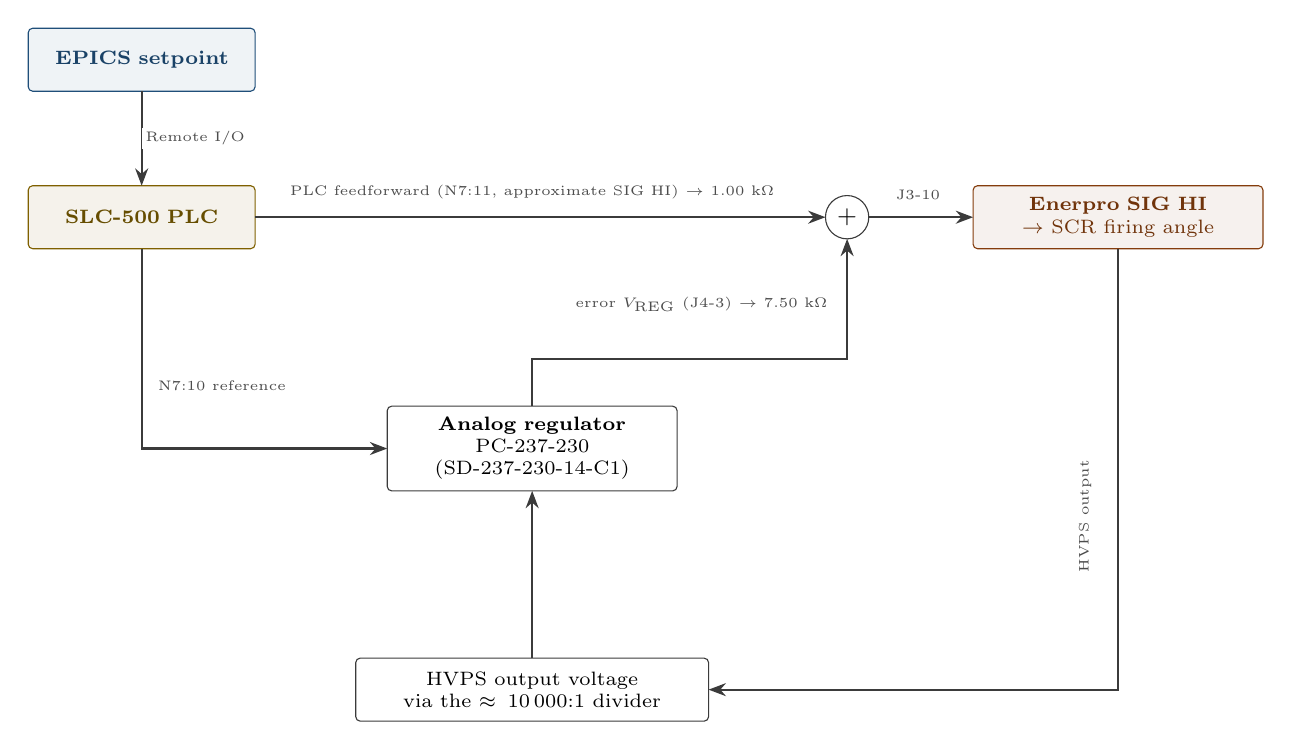
\begin{tikzpicture}[font=\scriptsize,x=1mm,y=1mm,every node/.style={outer sep=0pt}]
\tikzset{sum/.style={draw=cNeut,circle,inner sep=0pt,minimum size=5.5mm,font=\small}}

\node[ctrl,text width=26mm,anchor=west] (eps) at (8,0)   {\textbf{EPICS setpoint}};
\node[plc,text width=26mm,anchor=west]  (plc) at (8,-20)  {\textbf{SLC-500 PLC}};
\draw[sig] (eps.south) -- node[right,tag] {Remote I/O} (plc.north);

\node[sum]                              (sum) at (112,-20) {$+$};
\node[pwr,text width=34mm,anchor=west]  (ener) at (128,-20)
  {\textbf{Enerpro SIG HI}\\ $\rightarrow$ SCR firing angle};

% feedforward straight along the top
\draw[sig] (plc.east) -- (sum.west);
\draw[sig] (sum.east) -- (ener.west);
\node[tag,anchor=south] at (72,-18.2)
  {PLC feedforward (N7:11, approximate SIG HI) $\rightarrow$ 1.00 k$\Omega$};
\node[tag,anchor=south] at (121,-18.2) {J3-10};

% reference down and across into the regulator
\node[blk,text width=34mm,anchor=north] (reg) at (72,-44)
  {\textbf{Analog regulator}\\ PC-237-230\\ (SD-237-230-14-C1)};
\draw[sig] (plc.south) |- (reg.west);
\node[tag,anchor=south west] at (24,-42.5) {N7:10 reference};

% error up from the regulator into the summing junction
\draw[sig] (reg.north) -- ++(0,6) -| (sum.south);
\node[tag,anchor=south east] at (110,-32.5)
  {error $V_\text{REG}$ (J4-3) $\rightarrow$ 7.50 k$\Omega$};

% feedback: HVPS output through the divider back into the regulator
\node[blk,text width=42mm,anchor=north] (div) at (72,-76)
  {HVPS output voltage\\ via the $\approx 10\,000{:}1$ divider};
\draw[sig] (div.north) -- (reg.south);
\draw[sig] (ener.south) |- (div.east);
\node[tag,rotate=90,anchor=south] at (143.5,-58) {HVPS output};
\end{tikzpicture}
\end{fitpicture}
\caption{HVPS analog voltage regulation loop.  The analog regulator card
  compares the PLC reference with the HVPS output voltage feedback and
  generates a \emph{bipolar} error signal; that error is weighted and added to
  the PLC's \emph{unipolar} feedforward output to form SIG HI.  Power-line
  harmonics are clearly visible on the error signal in normal
  operation.}\label{fig:regulation-loop}
\end{figure}

The analog regulator card (PC-237-230, drawing SD-237-230-14-C1) compares the PLC reference with the HVPS output voltage feedback and generates a bipolar error signal. That error leaves the card on \textbf{J4-3} as $V_\text{REG}$ and is combined with the PLC's unipolar feedforward output ($V_\text{PLC}$, Slot-8 Output 1) in a \textbf{passive resistive combiner} --- 7.50 kΩ on the regulator card, 1.00 kΩ in series with the PLC wire --- whose junction is the Enerpro SIG HI input on \textbf{J3-10} \R{72}:
\[
  V_\text{SIG HI} = \tfrac{1}{8.5}\,V_\text{REG} + \tfrac{7.5}{8.5}\,V_\text{PLC}
               = 0.1176\,V_\text{REG} + 0.8824\,V_\text{PLC},
\]
with a source resistance of 882.4 Ω. The feedforward therefore sets the operating point and the regulator only trims it: at the documented $V_\text{PLC}=4.4538$ V the error amplifier's ±14 V swing maps to ±1.6464 V at SIG HI \R{72}. Power-line harmonics are clearly visible on the error signal in normal operation \R{40}.


\subsection{Terminal Strips and External Connections}\label{sec:terminal-strips}

The inventory below follows the source drawings and analysis; incomplete or conflicting terminal assignments still require a field record.\openitem{O4}\openitem{O9}

Internal wiring in the controller enclosure is organized on numbered terminal strips (reference drawing WD-730-790-02-C6 \R{15}). The strips identified in the original PPS wiring trace \R{25} are:

\begin{longtable}[]{@{}P{\dimexpr 0.1169\linewidth-1.333\tabcolsep\relax}P{\dimexpr 0.6540\linewidth-1.333\tabcolsep\relax}P{\dimexpr 0.2291\linewidth-1.333\tabcolsep\relax}@{}}
\toprule\noalign{}
Terminal strip & Function & External cable \\
\midrule\noalign{}
\endhead
\bottomrule\noalign{}
\endlastfoot
TS-2 & Control power supply distribution --- system common, ± rails, status & Internal \\
TS-3 & \textbf{Voltage Monitor.} Drawn on WD-730-790-02-C6 \R{63} directly against a block titled "PEP2 RF SYSTEM KLY PS MONITOR BD SD-730-793-12" and labeled VOLTAGE MONITOR. Terminals: DC VOLTAGE *1, DC VOLTAGE *2, COM, VOLTS, AMPS, COM, −15 V, +15 V, CURRENT 5A/V & Internal \\
TS-4 & Transformer interlocks & To HVPS tanks \\
TS-5 & Contactor controls, 15 terminals (B118 → Switchgear) & Belden 83715 (15C \#16 Teflon) \\
TS-6 & Grounding tank / Termination Tank, 21 terminals (B118 → B132) & Belden 83709 (9C \#16 Teflon) + Belden 83715 \\
TS-7 & Power distribution & Internal \\
TS-8 & PPS permits --- PPS 1 on terminal 1, PPS 2 on terminal 3, common on terminal 6 & From PPS GOB1208PNE connector \\
\end{longtable}

\textbf{PPS status indication} is \emph{not} on a terminal strip: the four external status LEDs (two green, two red) on the top left of the controller enclosure are wired to an \textbf{AMP 8-pin connector, J2} \R{25}. WD-730-790-02-C6 \R{63} draws the four LEDs between the mating pair \textbf{AMP-8PINM P2} (LED pigtails) and \textbf{AMP-8PIN J2} (cable), and labels them individually: \textbf{PPS1 LED1 GRN, PPS2 LED2 GRN, PPS3 LED3 RED, PPS4 LED4 RED}. The \textbf{PPS GOB1208PNE} connector appears alongside them on the same sheet.

\subsubsection{What the four lamps are wired to}

PPS pin pairing and readback excitation need verification against installed behavior.\openitem{O6}

Each lamp is a bare LED with its anode on one PPS circuit node and its cathode on the system common (GOB pin \textbf{H} --- TS-5 1/8, TS-2 2/4/6, TS-6 2). The anode assignments below are given identically by the drawing \R{63} and by the terminal-by-terminal trace \R{25}, down to the cable color code.

\begin{longtable}[]{@{}P{\dimexpr 0.1350\linewidth-1.600\tabcolsep\relax}P{\dimexpr 0.1450\linewidth-1.600\tabcolsep\relax}P{\dimexpr 0.0600\linewidth-1.600\tabcolsep\relax}P{\dimexpr 0.3100\linewidth-1.600\tabcolsep\relax}P{\dimexpr 0.3500\linewidth-1.600\tabcolsep\relax}@{}}
\toprule\noalign{}
Lamp & J2 anode / cathode & Pin & Circuit the anode sits on & Lamp follows \\
\midrule\noalign{}
\endhead
\bottomrule\noalign{}
\endlastfoot
\textbf{PPS1 LED1} \emph{green} & 1 (RED) / 2 (RED/BLK) & B & Chain-1 contactor readback; distinguish disconnect-panel TB2 from HQ3 TB2 (\cref{fig:pps-readback}) & Intended closed readback for contactor open; excitation and pin pairing unverified \\
\textbf{PPS2 LED2} \emph{green} & 3 (BLU) / 4 (BLK) & D & Chain-2 grounding readback: TS-6 11--12 $\rightarrow$ Ross grounding-switch auxiliary contact & Readback loop made: grounding switch \textbf{CLOSED}, HV bus grounded \\
\textbf{PPS3 LED3} \emph{red} & 5 (WHT) / 6 (WHT/BLK) & G & \textbf{PPS 2 enable}: TS-8 3, and SLC-500 slot 6 IB16 \textbf{IN15} (drawn "PPS \#2" on \R{63}) & PPS is granting the Chain-2 permit: grounding switch may be held open \\
\textbf{PPS4 LED4} \emph{red} & 7 (GRN) / 8 (GRN/BLK) & E & \textbf{PPS 1 enable}: TS-8 1, and SLC-500 slot 6 IB16 \textbf{IN14} (drawn "PPS \#1" on \R{63}) & PPS is granting the Chain-1 permit: contactor may close \\
\end{longtable}

These indicators are hardwired to PPS circuit nodes rather than driven by PLC outputs \R{25}, \R{63}. That does not make them independent proof of contact position or absence of voltage: illumination depends on external circuit excitation, common-return integrity and the unconfirmed PPS pin assignments.

\subsubsection{Indicator interpretation limits}

The table gives the intended interpretation of the circuit nodes. A dark lamp can indicate a missing permit, an open return, absent readback excitation or a failed indicator. A permit and its readback may coexist during a transition. These observations alone neither isolate a fault nor authorize access. Record all four lamp states against verified contact positions during the PPS validation walk-down.

The adjacent local control panel has a separate \textbf{PPS PERMIT} lamp on the PPS 2 line (GOB pin G), in series with the emergency-off contact \R{63}. It does not indicate both PPS channels. The PPS 1 line also enters the local emergency-off/key-switch circuit \R{25}.

\begin{keynote}
\textbf{Verification limits}: TS-1 is unidentified; TS-5 has conflicting source labels. The TS-5/TS-6/TS-8 trace in \R{25} needs verification against the installed system. See \hyperref[sec:open-items]{Open Items}, O1, O4, O6 and O9.
\end{keynote}


\section{Enerpro SCR Firing System}\label{sec:enerpro}

\subsection{Overview}

The documented board set is an \textbf{Enerpro FCOG6100 Rev K with an FCOAUX60 Rev D auxiliary firing board} \R{40}. The supply has two phase-shifted six-pulse power bridges, but the vendor schematic describes FCOAUX60 as an auxiliary gate-drive board, not a standalone 30° delay generator \R{13}, \R{28}.

\textbf{For the upcoming upgrade.} The \textbf{Enerpro FCOG1200} is a genuine 12-pulse board and is the \emph{replacement} selected for the HVPS controller upgrade; it is not installed. Everything in this section describes the FCOG6100 + FCOAUX60 set that is in service today.


\subsection{Current Hardware}

\begin{longtable}[]{@{}P{\dimexpr 0.2184\linewidth-1.600\tabcolsep\relax}P{\dimexpr 0.1757\linewidth-1.600\tabcolsep\relax}P{\dimexpr 0.1159\linewidth-1.600\tabcolsep\relax}P{\dimexpr 0.1948\linewidth-1.600\tabcolsep\relax}P{\dimexpr 0.2952\linewidth-1.600\tabcolsep\relax}@{}}
\toprule\noalign{}
Board & Model & Revision & Serial Numbers & Schematic \\
\midrule\noalign{}
\endhead
\bottomrule\noalign{}
\endlastfoot
Main firing boards & Enerpro FCOG6100 & Rev. K & SPEAR1: 41506 in \R{40}, 41504 in \R{72}; SPEAR2: 50470 & Enerpro E128; SLAC SD-237-230-12-R0 \R{13} \\
Auxiliary firing boards & Enerpro FCOAUX60 & Rev D & SPEAR1: 03198; SPEAR2: 03813 & \R{40}, \R{72} \\
\end{longtable}

\subsubsection{The regulator board and how SIG HI is actually formed}

SIG HI is formed in \textbf{two stages}. The SLAC-designed regulator card \textbf{SD-237-230-14-C1} (board designation PC-237-230) first selects a single control output $V_\text{REG}$ from its two internal loops; $V_\text{REG}$ is then resistively summed with the PLC feedforward to form the voltage actually presented to the Enerpro board (\cref{sec:analog-regulation}). The card's internal architecture is documented in detail by J. Sebek \R{72}, and three features of it are operationally important.

\textbf{(a) The card's two internal loops are combined by minimum-select, not by addition.} The board has two analog control chains --- one for the negative output \emph{voltage}, one for the positive input \emph{current} --- processed through identical signal-conditioning and error-amplifier stages. They are combined through a \textbf{non-linear diode "summing junction"} in which the \textbf{anodes of two diodes are tied together}. The \emph{lower} of the two cathode voltages wins and sets the common anode voltage, which becomes the card's control output $V_\text{REG}$ on J4-3. A 15 V DC supply through a 10 kΩ resistor keeps the conducting diode biased, and a \textbf{10 V Zener} clamps the anode. In other words the two loops compete and \textbf{whichever demands less output takes control} --- the classic voltage-or-current-limit arrangement.

\textbf{(b) Voltage regulation dominates at the documented operating point.} The AC-current reference at J4-2 (IL1) is the Enerpro +5 V reference. With the approximately 2 V current readback in \R{72}, the current error amplifier saturates positive and does not win the minimum-select. This operating-point analysis does \emph{not} prove that it can never take control at higher current. The separate overcurrent comparator remains a protection function; its as-set threshold requires verification.

\textbf{(c) AC and DC current are separate measurements.} The regulator uses rectified 300:5 input CT signals and a drawing-stated 0.5 Ω burden \R{67}, \R{70}. The Danfysik transducer separately measures cathode DC current. Confirm the burden and the Slot-9 input mapping, for which \R{72} contains conflicting prose and table entries.\openitem{O10}

\paragraph{Signal path summary}\label{signal-path-summary}

\begin{longtable}[]{@{}P{\dimexpr 0.2524\linewidth-1.000\tabcolsep\relax}P{\dimexpr 0.7476\linewidth-1.000\tabcolsep\relax}@{}}
\toprule\noalign{}
Signal & Path \\
\midrule\noalign{}
\endhead
\bottomrule\noalign{}
\endlastfoot
Voltage reference (setpoint) & AB \textbf{Slot-8 Output 0} → \textbf{J4-1 / J4-7}. \emph{On the board schematic this input is confusingly labeled "POS. VOLTAGE LIMIT COMMAND"; it is the reference voltage input, not a limit} \R{72} \\
HV readback & Voltage dividers (\cref{sec:hvps-components}) → \textbf{J1A / J1B} "NEG. VOLTAGE SENSE" → INA117 → error amplifier \\
Voltage monitor out & BUF634 → 1 kΩ → \textbf{J3-1} → AB \textbf{Slot-8 Input 0} \\
Current monitor out & BUF634 → \textbf{J3-2} → AB \textbf{Slot-9 In-0}, per the measurement table in \R{72}; that source's prose says In-1. Confirm the installed connection against \R{63}. \\
Current reference & Enerpro +5 V reference → \textbf{J4-2 (IL1)} \\
Card control output & Diode minimum-select → buffer → \textbf{J4-3} as $V_\text{REG}$; also read back on AB \textbf{Slot-8 Input 1} \R{72} \\
Enerpro SIG HI & $V_\text{REG}$ through 7.50 kΩ on the card, summed with the PLC feedforward (AB \textbf{Slot-8 Output 1}) through a 1.00 kΩ series resistor → \textbf{J3-10} on the Enerpro board \\
\end{longtable}

\paragraph{Loop dynamics}\label{loop-dynamics}

The voltage input network has a nominal 0.01 s time constant (15.9 Hz corner). With $R_{FB1}=10.0$ kΩ, $C_{FB1}=2.0$ µF and $C_{FB2}=1.0$ nF, the error amplifier contributes an integrator, a 7.96 Hz zero and a 15.9 kHz pole \R{72}. Integral action removes steady-state error only for a stable, unsaturated closed loop; these component values alone do not establish whole-station bandwidth or stability.

\paragraph{Protection thresholds}\label{protection-thresholds}

The overvoltage comparator is adjustable from 2 V to 12 V, approximately 20 kV to 120 kV at the nominal divider scale. Trip states latch in a CD4044B. The cited sources do not supply accepted and as-found voltage/current trip settings.

\paragraph{Test points}\label{test-points}

\begin{longtable}[]{@{}ll@{}}
\toprule\noalign{}
TP & Measures \\
\midrule\noalign{}
\endhead
\bottomrule\noalign{}
\endlastfoot
TP1 & Output of the current difference amplifier \\
TP2 & Output of the over-current comparator \\
TP4 & Inverted voltage difference of the negative voltage sense \\
TP5 & Output of the inverting error amplifier \\
TP8 & Output of the over-voltage comparator \\
TP9 & Inverted input of the voltage reference \\
TP10 & Over-voltage threshold setting \\
TP11 & Over-current threshold setting \\
TP12 & Inverted reference value generated by the Enerpro board \\
\end{longtable}

\subsection{Phase References}\label{sec:phase-references}

Enerpro firing boards normally take their phase references from the \emph{rectifier transformer secondaries}. The SPEAR3 HVPS cannot do this: there are no accessible secondary references, so the timing is instead derived from \textbf{monitor windings on the legs of the phase-shifting transformer T0}. Those windings lead one rectifier transformer primary by 15° and lag the other by 15° --- they are not in phase with either bridge.

Measured characteristics of these references, on both SPEAR1 and SPEAR2 \R{40}:

\begin{longtable}[]{@{}P{\dimexpr 0.4256\linewidth-1.000\tabcolsep\relax}P{\dimexpr 0.5744\linewidth-1.000\tabcolsep\relax}@{}}
\toprule\noalign{}
Property & Value \\
\midrule\noalign{}
\endhead
\bottomrule\noalign{}
\endlastfoot
Waveform & Sinusoidal, ≈ \textbf{190 V peak-to-peak} \\
Source impedance at the HVPS & 500 Ω \\
Voltage ratio of the monitor windings & ≈ 100:1 (125 V φ--φ for 12.5 kV φ--φ), 5 A RMS rating \R{22} \\
\end{longtable}

On the installed FCOG6100 these three references enter through \textbf{connector J5} as off-board phase references and are scaled by the on-board resistors \textbf{R37, R38 and R39} (J5-1 = R37 = phase A, J5-3 = R38 = phase B, J5-5 = R39 = phase C). Inside the board the references are pulled to +5 V DC through 15 kΩ resistors in RN1, divided by RC networks, and squared up by LM324 comparators in the phase-detection circuitry \R{40}.

\textbf{Resistor value --- standard vs. SLAC.} The Enerpro schematic \R{13} gives R31--R39 as \textbf{1.9 MΩ, ½ W, 1\%, RN70} in its parts list, and Note 10 states \emph{"FOR OFF-BOARD PHASE REFERENCES: INSTALL R37-R39 AND J5. OMIT R31-R33 AND T1."} SLAC's boards have \textbf{R37--R39 changed to 200 kΩ} to suit the ≈190 Vpk-pk monitor-winding reference, which is much lower than the line voltages the standard 1.9 MΩ value assumes; Sebek works the Thevenin equivalent using 200.5 kΩ (200 kΩ plus the 500 Ω source impedance) \R{40}. Both values are correct for their respective contexts and must not be interchanged.

\textbf{Connector roles on the FCOG6100} (from the schematic notes \R{13}):

\begin{longtable}[]{@{}ll@{}}
\toprule\noalign{}
Connector & Role \\
\midrule\noalign{}
\endhead
\bottomrule\noalign{}
\endlastfoot
J5 & Off-board phase references (Note 10) --- the path used at SPEAR3 \\
J7 & Provided for \textbf{test} reference inputs (Note 11) \\
J8 & Cable to the \textbf{FCOAUX60} auxiliary board, for gating paralleled SCRs (Note 12) \\
J10 & 50/60 Hz jack (added at revision J) \\
J1/P1, J2/P2 & Gate drive: +A/+B/+C for line-to-load SCRs; −A/−B/−C for load-to-line SCRs \\
\end{longtable}

A \textbf{single} on-board jumper block, \textbf{PP1} (AMP 435704-8), carries both of the drawing's configuration tables \R{13}. Positions \textbf{1--6} set the \textbf{phase reference}: 1,2,3 open with 4,5,6 closed gives 0°, the reverse gives −30°. Positions \textbf{7--8} set the \textbf{gate pulse profile}: 7 open / 8 closed = 120° burst; both closed = 2×30° bursts; 7 closed / 8 open = 2×60° spaced pulses; both open = not used. Drawing note 9 directs the shunts to be set from those tables. The SIG HI input path is buffered by U6 with span (R42) and bias (R43) trim; Note 18 records that R52 = 150 kΩ suits 0 V \textless{} SIG HI \textless{} 5.0 V while R52 = 249 kΩ suits 0.9 V \textless{} SIG HI \textless{} 5.9 V.

\begin{keynote}
\textbf{The "Phase Reference Adapter" is an upgrade item, not legacy hardware.} The FCOG1200 has no place for input resistors between its J7 connector and the phase-detection circuitry, so a small adapter board is being designed for the upgrade: three inputs, \textbf{six} resistors, six outputs --- 3 × 576 kΩ to J7 pins 1--3 and 3 × 200 kΩ to J7 pins 4--6, with Enerpro replacing RN4A--C with 66.5 kΩ and RN4D--F with 287 kΩ so that one triplet is advanced and the other retarded by 15°. The mating connector is TE 3-640440-8 (Enerpro C2MTAPLG08). None of this exists in the installed system \R{58}.
\end{keynote}

\subsection{Legacy vs. Upgrade Firing Board}

\begin{longtable}[]{@{}P{\dimexpr 0.2490\linewidth-1.333\tabcolsep\relax}P{\dimexpr 0.3582\linewidth-1.333\tabcolsep\relax}P{\dimexpr 0.3929\linewidth-1.333\tabcolsep\relax}@{}}
\toprule\noalign{}
& \textbf{Installed (legacy)} & \textbf{Selected for upgrade} \\
\midrule\noalign{}
\endhead
\bottomrule\noalign{}
\endlastfoot
Board(s) & FCOG6100 Rev K (six-pulse) + FCOAUX60 Rev D (auxiliary drive) & FCOG1200 Rev L (native 12-pulse) \\
Phase reference entry & J5, with on-board R37--R39 = 200 kΩ & J7, via a custom external adapter (\cref{sec:phase-references}) \\
Phase-reference matching & Installed phasing and trigger distribution require verification & Proposed RN4 modifications with matched 0.033 μF capacitors \R{58} \\
Auto-balance & Not used & On-board trimpot adjustment only (no independent bridge monitoring available) \\
SIG HI input & Terminated into an inverting op-amp input held at +5 V DC (R49/U6) & High-impedance buffer input, nominal 0.8--5.8 V range \\
Status & In service; obsolete, limited vendor support & Not yet procured/installed \\
\end{longtable}


\section{Arc Protection and Crowbar System}\label{sec:arc-protection}

\subsection{Four-Layer Protection Architecture}

The HVPS implements a 4-layer arc protection system to protect the klystron from destructive energy discharge during arcs. \textbf{The response times below distinguish signal latency from physical response} --- the two differ by orders of magnitude, and it is the physical response that bounds the protection:

\begin{longtable}[]{@{}Q{\dimexpr 0.08\linewidth-1.600\tabcolsep\relax}Q{\dimexpr 0.12\linewidth-1.600\tabcolsep\relax}Q{\dimexpr 0.12\linewidth-1.600\tabcolsep\relax}Q{\dimexpr 0.16\linewidth-1.600\tabcolsep\relax}Q{\dimexpr 0.52\linewidth-1.600\tabcolsep\relax}@{}}
\toprule\noalign{}
Layer & Protection & Signal latency & Physical response & Mechanism \\
\midrule\noalign{}
\endhead
\bottomrule\noalign{}
\endlastfoot
1 & SCR firing inhibit & Not measured here & \textbf{4--8 ms}, PEP-II result & Inhibit rectification and freewheel primary-inductor current through a conducting phase leg. Interruption depends on AC phase and commutation \R{6}. \\
2 & Crowbar firing & Not measured here & \textbf{≈ 10 μs}, PEP-II result & Trigger four series crowbar stacks; the quoted delay is to conduction, not the total sensor-to-trip latency \R{6}. \\
3 & Filter capacitor isolation & --- & Passive circuit response & Series filter resistors limit energy delivered from the capacitor bank during an arc. \\
4 & Cable termination inductors & --- & Passive circuit response & Limit cable-discharge current. The 1997 design uses 200 μH; the SPEAR3 grounding-tank drawing specifies 350 μH, 40 A \R{6}, \R{62}. \\
\end{longtable}

Layers 1 and 2 are actively commanded --- in the legacy system by the \textbf{Fast Interlock Chassis 340-308} and, on a slower supervisory path, by the \textbf{SLC-500 HVPS PLC}. Layers 3 and 4 are passive properties of the circuit topology. 

\subsection{Klystron Arc Energy Budget}

The PEP-II paper cites two klystron protection criteria: arc energy below \qty{60}{\joule} and $I^2t$ below \qty{40}{\ampere\squared\second} \R{6}. These are different quantities, not interchangeable limits without an arc model. Its reported results are:

\begin{longtable}[]{@{}ll@{}}
\toprule\noalign{}
Condition & Energy reaching the klystron \\
\midrule\noalign{}
\endhead
\bottomrule\noalign{}
\endlastfoot
Crowbar operating, PEP-II test configuration & \textbf{\textless{} 5 J} \\
Crowbar disabled, general result in abstract & \textbf{\textless{} 40 J} \\
Crowbar disabled, with described termination inductors & \textbf{\textless{} 20 J} \\
\end{longtable}

The rectifier/resistor/filter arrangement limits energy delivery even without crowbar action. These published design results are \textbf{not a fault-tolerance certification of the installed SPEAR3 units}; installed component condition, trigger timing and cable configuration require their own acceptance evidence. The 200 μH termination inductors described in \R{6} also differ from the 350 μH drawing value in \R{62}.


\FloatBarrier\clearpage
\part{PROTECTION AND SAFETY SYSTEMS}

Protection is distributed among the Fast IC/AIM hardware, the independent VXI MPS shutoff interface, the RF MPS PLC, the HVPS PLC and IOC supervision. PPS controls the primary contactor and grounding-switch functions separately from equipment protection. Hardware actions do not wait for the IOC, but complete installed-path latencies are not established by the cited sources. The PEP-II power-stage results in \cref{sec:arc-protection} must not be used as end-to-end SPEAR3 trip times.

This part of Doc L summarizes the three protection subsystems (PPS, RF MPS, and Fast IC / interlock chain).


\section{Personnel Protection System (PPS) Interface}\label{sec:pps}

\subsection{Overview}

The PPS interface controls two critical safety functions: the HV vacuum contactor (which connects 12.47 kV AC power to the HVPS) and the Ross grounding switch (which grounds the HVPS output for safe access).

\textbf{Review priority}: Both chains involve the SLC-500 PLC. The contactor chain also has a hardware PPS supply dependency, whereas the documented Ross-switch output has no separate series PPS interrupt \R{25}. This is a personnel-protection review issue; compliance and access authorization must be determined by the responsible PPS authority, not inferred from this architecture summary.

\subsection{Legacy PPS Chain 1: HV Contactor}

\Cref{fig:pps-chains} shows both legacy chains: Chain 1, described here, interrupts the 12.47 kV supply at the vacuum contactor; Chain 2 grounds the HVPS output at the Ross switch.

\begin{figure}[p]\centering
\begin{fitpicture}% !TeX root = ../L_legacy_system_architecture.tex
% The two legacy PPS chains, side by side.  Both pass through the SLC-500 PLC
% -- the compliance issue called out in the text.
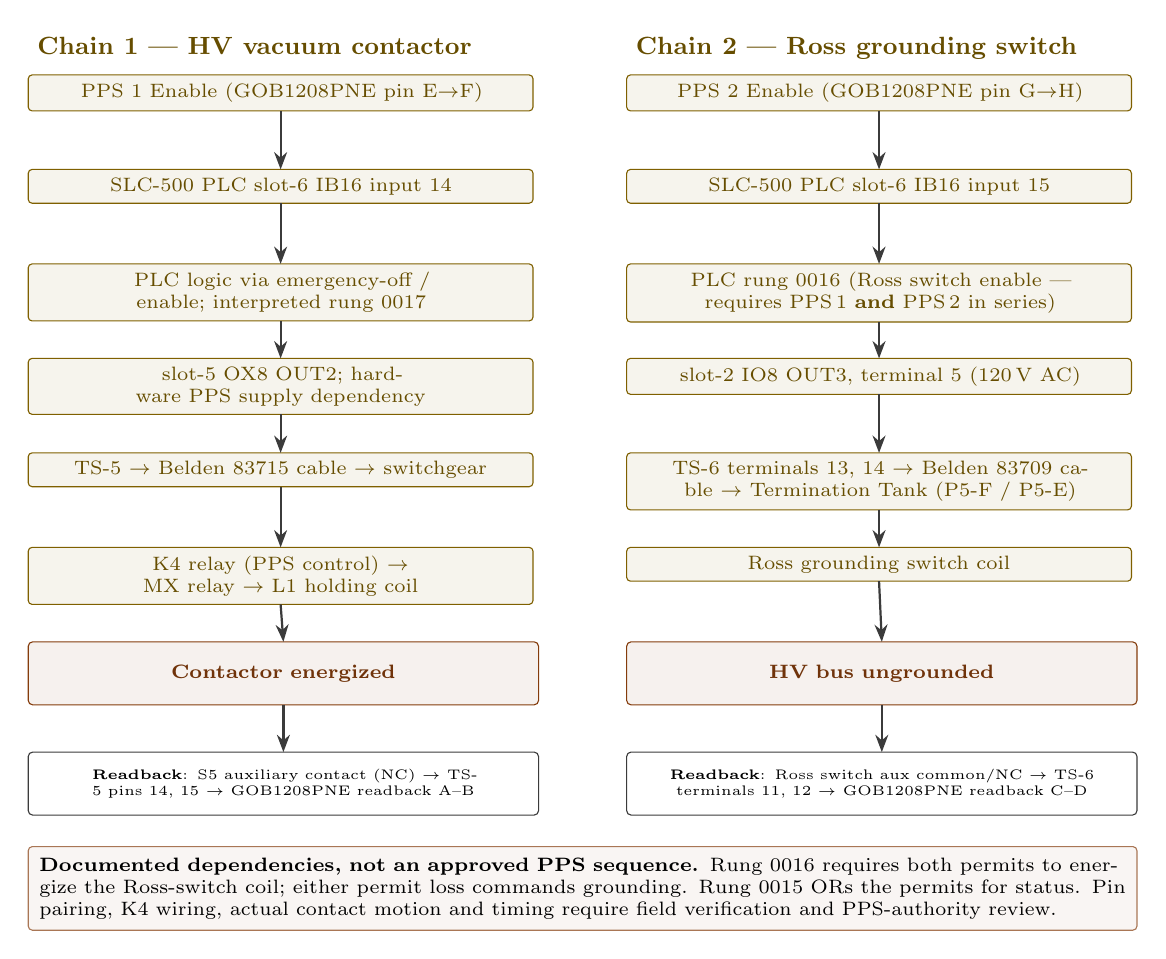
\begin{tikzpicture}[font=\scriptsize,x=1mm,y=1mm,every node/.style={outer sep=0pt}]
\tikzset{ppsbox/.style={draw=cPlc,fill=cPlc!7,rounded corners=1.4pt,
                      text=cPlc!80!black,align=center,inner sep=3pt,
                      font=\scriptsize,text width=62mm}}

% ---------------- Chain 1 -------------------------------------------------
\node[font=\small\bfseries,anchor=north west,text=cPlc!80!black] at (0,4)
  {Chain 1 --- HV vacuum contactor};
\foreach \i/\y/\t in {%
  1/-2/{PPS 1 Enable (GOB1208PNE pin E$\rightarrow$F)},
  2/-14/{SLC-500 PLC slot-6 IB16 input 14},
  3/-26/{PLC logic via emergency-off / enable; interpreted rung 0017},
  4/-38/{slot-5 OX8 OUT2; hardware PPS supply dependency},
  5/-50/{TS-5 $\rightarrow$ Belden 83715 cable $\rightarrow$ switchgear},
  6/-62/{K4 relay (PPS control) $\rightarrow$ MX relay $\rightarrow$ L1 holding coil}}
  {\node[ppsbox,anchor=north west] (a\i) at (0,\y) {\t};}
\foreach \a/\b in {1/2,2/3,3/4,4/5,5/6}{\draw[sig] (a\a.south) -- (a\b.north);}
\node[pwr,text width=62mm,anchor=north west] (a7) at (0,-74) {\textbf{Contactor energized}};
\draw[sig] (a6.south) -- (a7.north);
\node[blk,text width=62mm,anchor=north west,font=\tiny] (a8) at (0,-88)
  {\textbf{Readback}: S5 auxiliary contact (NC) $\rightarrow$ TS-5 pins 14, 15
   $\rightarrow$ GOB1208PNE readback A--B};
\draw[sig] (a7.south) -- (a8.north);

% ---------------- Chain 2 -------------------------------------------------
\node[font=\small\bfseries,anchor=north west,text=cPlc!80!black] at (76,4)
  {Chain 2 --- Ross grounding switch};
\foreach \i/\y/\t in {%
  1/-2/{PPS 2 Enable (GOB1208PNE pin G$\rightarrow$H)},
  2/-14/{SLC-500 PLC slot-6 IB16 input 15},
  3/-26/{PLC rung 0016 (Ross switch enable --- requires PPS\,1 \textbf{and} PPS\,2 in series)},
  4/-38/{slot-2 IO8 OUT3, terminal 5 (\qty{120}{\volt} AC)},
  5/-50/{TS-6 terminals 13, 14 $\rightarrow$ Belden 83709 cable $\rightarrow$ Termination Tank (P5-F / P5-E)},
  6/-62/{Ross grounding switch coil}}
  {\node[ppsbox,anchor=north west] (b\i) at (76,\y) {\t};}
\foreach \a/\b in {1/2,2/3,3/4,4/5,5/6}{\draw[sig] (b\a.south) -- (b\b.north);}
\node[pwr,text width=62mm,anchor=north west] (b7) at (76,-74) {\textbf{HV bus ungrounded}};
\draw[sig] (b6.south) -- (b7.north);
\node[blk,text width=62mm,anchor=north west,font=\tiny] (b8) at (76,-88)
  {\textbf{Readback}: Ross switch aux common/NC $\rightarrow$ TS-6 terminals 11, 12
   $\rightarrow$ GOB1208PNE readback C--D};
\draw[sig] (b7.south) -- (b8.north);

% ---------------- compliance note ----------------------------------------
\node[anchor=north west,text width=138mm,font=\scriptsize,align=left,
      draw=cPwr!70,fill=cPwr!5,rounded corners=1.5pt,inner sep=4pt] at (0,-100)
  {\textbf{Documented dependencies, not an approved PPS sequence.}
   Rung 0016 requires both permits to energize the Ross-switch coil; either
   permit loss commands grounding. Rung 0015 ORs the permits for status.
   Pin pairing, K4 wiring, actual contact motion and timing require field
   verification and PPS-authority review.};
\end{tikzpicture}
\end{fitpicture}
\caption{The two legacy PPS chains.}\label{fig:pps-chains}
\end{figure}
\clearpage

\subsection{Legacy PPS Chain 2: Ross Grounding Switch}

\begin{keynote}
\textbf{Logic}: Rung 0016 requires PPS 1 \emph{and} PPS 2, with other conditions, to energize the Ross-switch coil. Removing either permit commands de-energization; actual grounding still depends on output and switch operation. Rung 0015 ORs the permits into a status bit, so "PPS ON" is not proof that both permits are present \R{25}, \R{26}.
\end{keynote}

\begin{keynote}
\textbf{Pin-letter caveat}: The E--F/G--H enable and A--B/C--D readback assignments remain assumptions in \R{25}; see \hyperref[sec:open-items]{Open Items}, O6.
\end{keynote}

\subsection{Identified Issues}

The K4/RR interpretation requires an installed-wiring check.\openitem{O1}
The manual grounding-switch contact sense also differs between the schematic and the test-stand wiring drawing.\openitem{O2}

\begin{longtable}[]{@{}P{\dimexpr 0.1502\linewidth-1.333\tabcolsep\relax}P{\dimexpr 0.0967\linewidth-1.333\tabcolsep\relax}P{\dimexpr 0.7531\linewidth-1.333\tabcolsep\relax}@{}}
\toprule\noalign{}
Issue & Severity & Details \\
\midrule\noalign{}
\endhead
\bottomrule\noalign{}
\endlastfoot
PLC in PPS chain & Critical & Both PPS chains route through SLC-500 PLC ladder logic \\
PPS wiring exposed & High & PPS wires terminate on TS-5, TS-6 and TS-8 inside the HVPS controller enclosure, co-located with non-PPS wiring \\
Ross switch PLC dependency & High & Ross switch coil is driven by a PLC 120 VAC output (Slot-2 IO8 OUT3), with no hardware PPS element in series \\
K4/RR relay labels & Medium & \R{25} infers that the PPS/reset labels on WD-730-794-02-C0 are swapped and that K4 NO / 86 NC contacts are omitted from the MX path. Confirm the installed relay functions and issue reconciled drawings; the note explicitly leaves field verification open. \\
Contactor re-close delay & Low & Because K4 removes all control power from the contactor controller, capacitor C6 must recharge before K3 can re-energize --- this is why the contactor takes several seconds to re-close after a PPS enable is restored \R{25} \\
Hardware obsolescence & High & SLC-500 and 1746 modules are end-of-life \\
\end{longtable}

\subsection{Relay Chain Details (Contactor Disconnect Panel)}

Confirm historical switchgear device/rating details, including the temperature sensor marked for later addition, against the installed equipment.
The SPEAR-only low-pressure switch on \R{68} also needs a verified test record.

\begin{longtable}[]{@{}P{\dimexpr 0.1168\linewidth-1.333\tabcolsep\relax}P{\dimexpr 0.7664\linewidth-1.333\tabcolsep\relax}P{\dimexpr 0.1168\linewidth-1.333\tabcolsep\relax}@{}}
\toprule\noalign{}
Component & Function & Type \\
\midrule\noalign{}
\endhead
\bottomrule\noalign{}
\endlastfoot
K4 & PPS Control Relay --- energized from OX8 OUT2 with the PPS common as its return; two NO contacts, one interrupting controller control power and one in series with the MX coil & Relay \\
MX & \textbf{Remote Control Relay, 24 V DC} \R{69} --- must be energized for K1 (and hence the L2 closing coil) and stays energized to hold L1 & Relay \\
RR & \textbf{Remote Reset Relay, 24 V DC} \R{69} --- its NC contact is in the TX latch chain; energizing RR clears a latched TX overcurrent trip & Relay \\
IP & \textbf{Interposing Relay, 24 V DC} \R{69} --- added at revision 2 of the original LBL drawing alongside 27, MX and RR. Not described in any derived note; presence at SPEAR3 unconfirmed & Relay \\
27 & \textbf{Under Voltage Relay} \R{69} & Relay \\
01 / LT & \textbf{Local Control Switch --- Trip} \R{69} & Switch \\
M & \textbf{Main operating and holding coils} \R{69} & Coil \\
TX & Auxiliary tripping relay --- summarizes the eight overcurrent protection relays (instantaneous 50A/B/C/N and time 51A/B/C/N) and latches; must be de-energized for L1 to hold & Relay \\
L2 & Closing coil --- high-power coil that initially closes the vacuum contactor, fired from the stored-energy capacitor bank & Coil \\
L1 & Holding Coil --- maintains the vacuum contactor closed once L2 has closed it & Coil \\
S4, S5 & HQ3 auxiliary contacts on TB2 terminals 15--17 and 18--20, NO/COM/NC \R{66}. S5 supplies the PPS readback (\cref{fig:pps-readback}). Do not confuse HQ3 terminal numbering with the separately named disconnect-panel terminal block \R{67}. & Contact \\
Vacuum Contactor & Ross Eng. \textbf{HQ3}, P/N 813203. The original 1977 drawing lists 14.5 kV, 400 A, three poles, 50E fuses and 50/5 CTs \R{69}; these historical protection ratings are not an inventory of the installed SPEAR3 fuse/CT configuration. & HV contactor \\
Controller & Ross Eng. \textbf{HCA-1-A}, P/N 820360 --- contactor controller / energy-storage driver (\R{65} system view; \R{66} internal schematic) & Controller \\
\end{longtable}

\paragraph{Opening Timing}\label{opening-timing--from-the-drawings-own-sequence-of-operation-r65}

The original controller sequence \R{65} states:

\begin{longtable}[]{@{}P{\dimexpr 0.4847\linewidth-1.000\tabcolsep\relax}P{\dimexpr 0.5153\linewidth-1.000\tabcolsep\relax}@{}}
\toprule\noalign{}
Stage & Time \\
\midrule\noalign{}
\endhead
\bottomrule\noalign{}
\endlastfoot
Hold-in after loss of AC control voltage & \textbf{≥ 170 ms} \\
L1 holding solenoid dropout & within \textbf{1 cycle} (≈ 17 ms) \\
HV contacts clear & a further \textbf{½--1 cycle}, nominally at the first current zero \\
Loss of control power to interruption & Order 0.2 s from the stated stages, \textbf{not a maximum bound}; blocking and stored-energy conditions affect opening \\
Recharge before reclose is possible & \textbf{a few seconds} (K2 ready relay waits on the MT1 voltage sensor) \\
\end{longtable}

\begin{keynote}
\textbf{Blocking condition}: The original LBL drawing describes a 2000 A blocking threshold \R{69}. The later controller sequence states that BR can bypass normal opening commands while fault current persists \R{65}. Fuse coordination, installed pickup settings and PPS response under this condition require switchgear/PPS review; the historical drawing does not establish current settings or a maximum interruption time.
\end{keynote}

\paragraph{Stored Energy in the HCA-1-A Driver}\label{stored-energy-hazard-in-the-hca-1-a-driver-r66}

The HCA-1-A contains \textbf{300--400 V DC} stored-energy circuits. Its drawing describes door-interlock discharge within 5 s and passive decay to about 80 V in 5 minutes or 40 V in 10 minutes \R{66}. These are source-stated expectations, not verified discharge times for the installed unit. Do not use them as access criteria or as a substitute for an approved isolation/discharge procedure and absence-of-voltage testing.

The drawings agree on the internal HQ3 S5 contact and wire numbering. They do not establish a fully verified end-to-end connection to the external PPS chassis:

\begin{longtable}[]{@{}P{\dimexpr 0.0939\linewidth-1.333\tabcolsep\relax}P{\dimexpr 0.2391\linewidth-1.333\tabcolsep\relax}P{\dimexpr 0.6670\linewidth-1.333\tabcolsep\relax}@{}}
\toprule\noalign{}
Link & Drawing & What it establishes \\
\midrule\noalign{}
\endhead
\bottomrule\noalign{}
\endlastfoot
1 & Ross 713203 E-1 \R{66} & The HQ3 contactor brings out a spare auxiliary contact set \textbf{S5} on \textbf{TB2-18 (NO) / TB2-19 (COM) / TB2-20 (NC)} \\
2 & ID-308-801-06-C1 \R{68} & TB2-18, TB2-19 and TB2-20 carry \textbf{wires 20, 21 and 22} \\
3 & GP-439-704-02-C1 \R{65} & Wires \textbf{20, 21, 22} are the ones labeled \textbf{"PPS (CONTACTOR)"}, landing on \textbf{TB3-22, TB3-23, TB3-24} \\
4 & WD-730-790-01-C3 \R{67} & The Contactor Disconnect panel labels one auxiliary contact set \textbf{"CONTACTS PPS"} \\
\end{longtable}

\Cref{fig:pps-readback} draws these four links end to end.

\begin{figure}[tbp]\centering
\begin{fitpicture}% !TeX root = ../L_legacy_system_architecture.tex
% PPS contact readback trace, established by cross-reading four drawings.
% Links 1-3 are unambiguous; link 4 is corroborative only.
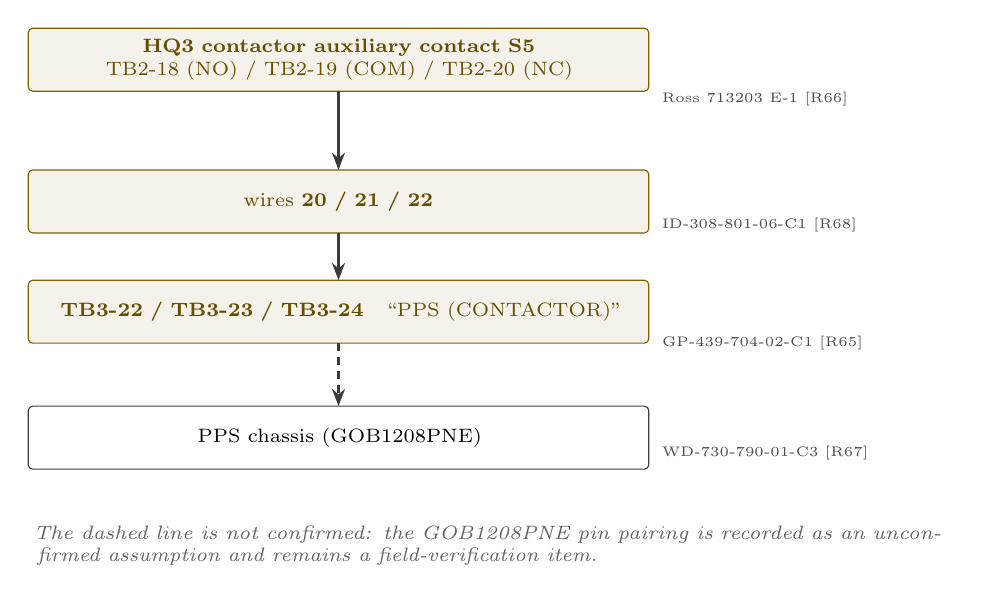
\begin{tikzpicture}[font=\scriptsize,x=1mm,y=1mm,every node/.style={outer sep=0pt}]
\node[plc,text width=76mm,anchor=north west] (n1) at (0,0)
  {\textbf{HQ3 contactor auxiliary contact S5}\\
   TB2-18 (NO) / TB2-19 (COM) / TB2-20 (NC)};
\node[plc,text width=76mm,anchor=north west] (n2) at (0,-18)
  {wires \textbf{20 / 21 / 22}};
\node[plc,text width=76mm,anchor=north west] (n3) at (0,-32)
  {\textbf{TB3-22 / TB3-23 / TB3-24}\quad``PPS (CONTACTOR)''};
\node[blk,text width=76mm,anchor=north west] (n4) at (0,-48)
  {PPS chassis (GOB1208PNE)};

\draw[sig] (n1.south) -- (n2.north);
\draw[sig] (n2.south) -- (n3.north);
\draw[sig,densely dashed] (n3.south) -- (n4.north);

\foreach \n/\y/\src in {n1/-9/{Ross 713203 E-1\ [R66]},
                        n2/-25/{ID-308-801-06-C1\ [R68]},
                        n3/-40/{GP-439-704-02-C1\ [R65]},
                        n4/-54/{WD-730-790-01-C3\ [R67]}}
  {\node[tag,anchor=west] at (80,\y) {\src};}

\node[lbl,anchor=north west,text width=118mm,align=left] at (0,-62)
  {The dashed line is not confirmed: the GOB1208PNE pin pairing is recorded as an unconfirmed
   assumption and remains a field-verification item.};
\end{tikzpicture}
\end{fitpicture}
\caption{PPS contact readback trace across four drawings.}\label{fig:pps-readback}
\end{figure}

\clearpage
\subsection{PPS Dual-Chain Interaction and Roles}

The contactor and grounding-switch chains perform \textbf{complementary functions}. Their documented operating directions are:

\begin{longtable}[]{@{}P{\dimexpr 0.1749\linewidth-1.333\tabcolsep\relax}P{\dimexpr 0.4266\linewidth-1.333\tabcolsep\relax}P{\dimexpr 0.3985\linewidth-1.333\tabcolsep\relax}@{}}
\toprule\noalign{}
& \textbf{Chain 1 --- HV Vacuum Contactor} & \textbf{Chain 2 --- Ross Grounding Switch} \\
\midrule\noalign{}
\endhead
\bottomrule\noalign{}
\endlastfoot
\textbf{Safety function} & Disconnect 12.47 kV AC primary power from HVPS & Ground the HVPS HV output bus for safe personnel access \\
\textbf{Operating state} & Coil energized → contactor \textbf{CLOSED} (12.47 kV connected) & Coil energized → switch held \textbf{OPEN} (HV bus not grounded) \\
\textbf{Safe-access state} & PPS 1 removed → K4 drops → L1 drops → contactor \textbf{spring-opens} → 12.47 kV disconnected & PPS 2 removed → 120 VAC removed → switch \textbf{spring-closes} → HV bus grounded \\
\textbf{Readback} & S5 NC auxiliary contact closed = contactor OPEN = 12.47 kV removed & Ross switch NC auxiliary contact closed = switch GROUNDED = HV bus grounded \\
\textbf{Fail-safe direction} & Lose power → contactor opens → safe & Lose power → switch closes to ground → safe \\
\end{longtable}

\textbf{Sequence not established here.} Because rung 0016 requires both permits, removing PPS 1 also commands the grounding-switch coil off. The sources do not support a sequence in which PPS 1 is removed, the supply is allowed to discharge, and only then PPS 2 is removed to initiate grounding. Actual contactor opening, grounding-switch closure, external PPS sequencing and access authorization require a validated end-to-end timing/logic record. No lamp or PLC bit alone proves absence of hazardous energy.
\openitem{O11}

\textbf{Dependency Comparison}:

\begin{longtable}[]{@{}P{\dimexpr 0.1596\linewidth-1.333\tabcolsep\relax}P{\dimexpr 0.4366\linewidth-1.333\tabcolsep\relax}P{\dimexpr 0.4038\linewidth-1.333\tabcolsep\relax}@{}}
\toprule\noalign{}
& \textbf{Chain 1} & \textbf{Chain 2} \\
\midrule\noalign{}
\endhead
\bottomrule\noalign{}
\endlastfoot
PLC dependency & PPS 1 routes through SLC-500 Rung 0017 & PPS 2 routes through SLC-500 Rung 0016 \\
Hardware fail-safe & \textbf{Present} --- OX8 relay input side wired to PPS 1 (24VDC). K4 cannot energize without PPS 1 even if PLC closes relay contact. & \textbf{Absent} --- IO8 OUT3 drives 120 VAC to Ross coil. PLC failure energized could hold switch open without PPS 2. \\
Residual review issue & Confirm the interpreted K4 wiring, contact behavior and blocking-relay conditions in the installed equipment & A PLC output remaining energized can leave the HV bus ungrounded despite a removed permit \\
\end{longtable}

The grounding switch returns toward ground on loss of \emph{coil power}; loss of a PPS logic signal is not equivalent if the PLC output remains energized. The legacy dependency is documented in \R{25}. The proposed replacement is outside this document's scope; see Doc 0.


\section{RF Machine Protection System (MPS)}\label{sec:rf-mps}

\subsection{Overview}

The RF MPS provides equipment/machine protection --- distinct from the personnel-safety PPS. It monitors klystron operating parameters and RF station conditions, removing permits to protect equipment from damage.

\subsection{Hardware Evolution}

\begin{longtable}[]{@{}P{\dimexpr 0.1518\linewidth-1.333\tabcolsep\relax}P{\dimexpr 0.3436\linewidth-1.333\tabcolsep\relax}P{\dimexpr 0.5046\linewidth-1.333\tabcolsep\relax}@{}}
\toprule\noalign{}
Era & Platform & Status \\
\midrule\noalign{}
\endhead
\bottomrule\noalign{}
\endlastfoot
\textbf{In service} & Allen-Bradley PLC-5 with 1771-series I/O; 1771-DCM Remote I/O adapter (rack 3) & Obsolete, no vendor support, but \textbf{this is the platform currently protecting the station} \\
Prepared replacement & Allen-Bradley ControlLogix 1756 (Rockwell conversion kit) & Hardware assembled, software written, tested on SPEAR3 \textbf{without RF power}. \textbf{Not yet in service}; will be commissioned as part of the LLRF upgrade \R{5} \\
\end{longtable}

\subsection{Protection Functions}

The RF MPS monitors and protects against:

\begin{itemize}
\tightlist
\item
  Excessive klystron collector power (cathode power minus RF output)
\item
  Excessive reflected power at any cavity
\item
  Waveguide arc conditions (via interlock chassis inputs)
\item
  Loss of cooling water
\item
  Klystron vacuum excursion
\item
  HVPS fault conditions
\end{itemize}

The original sources distinguish the following interfaces; they do \textbf{not} establish that one RF MPS relay drives three simultaneous, independent shutdown paths:
\openitem{O3}

\begin{itemize}
\tightlist
\item
  \textbf{RF MPS hardwired interface}: PLC/interlock signals connect to the ARC/Fast IC and AIM hardware. Confirm the per-fault SCR-inhibit and crowbar action in a consolidated trip truth table \R{21}, \R{53}, \R{79}.
\item
  \textbf{Remote I/O}: Status and permits are read by the IOC for alarms and sequencing. A serial status bit is not a direct hardware RF cutoff, and no fixed 10 ms response is established \R{60}.
\item
  \textbf{SPEAR MPS shutoff interface}: The VXI interlock module asserts \texttt{RF\_FAULT}, which directly inhibits RFP drive without waiting for EPICS. Its slot is 5 in the archived four-cavity configuration; \R{53} describes the earlier slot-6 implementation \R{60}.
\end{itemize}

\begin{keynote}
\textbf{HVPS PLC}: The SLC-500 independently monitors HVPS conditions and controls its enable outputs. The original PLC notes estimate a 5 ms program scan, with selected functions gated at 80 ms or longer intervals \R{37}. Neither number is a measured complete fault-response bound.
\end{keynote}

\subsection{MPS Wiring}

The repository contains 33 MPS drawing files, numbers 02--34 (number 06 is revision 01), covering cavity junctions, vacuum, cooling, analog/digital I/O, tuners, filament, optical interfaces and focus supplies \R{21}. They document wiring, not a complete PLC program or a validated per-fault trip truth table.


\section{Interlock Architecture and Signal Chain}\label{sec:interlocks}

\subsection{Overview}

The interlock system spans multiple hardware layers, from fast analog hardware interlocks to slow PLC-monitored conditions:

\begin{longtable}[]{@{}P{\dimexpr 0.1685\linewidth-1.500\tabcolsep\relax}P{\dimexpr 0.3258\linewidth-1.500\tabcolsep\relax}P{\dimexpr 0.2370\linewidth-1.500\tabcolsep\relax}P{\dimexpr 0.2687\linewidth-1.500\tabcolsep\relax}@{}}
\toprule\noalign{}
Layer & Speed & Hardware & Function \\
\midrule\noalign{}
\endhead
\bottomrule\noalign{}
\endlastfoot
Fast hardware & No installed end-to-end latency record & Fast IC, AIM, IQA and RFP & Hardware faults and RF-drive inhibit \\
RF MPS logic & Scan and I/O dependent; unmeasured here & PLC-5 & Equipment protection calculations \\
HVPS logic & Estimated 5 ms scan; timed functions differ \R{37} & SLC-500 & HVPS sequencing and monitoring \\
IOC supervision & Event/scan driven; shutdown includes explicit waits & VXI IOC / SNL & Sequencing, alarms and fault export \\
\end{longtable}

\subsection{Interlock Chassis}

The Local Control Chassis I/O and its relationship to the Fast IC remain unresolved.\openitem{O7}
Installed sensor mappings, masks, fiber endpoints and hardware response require proof-test records.

\begin{keynote}
\textbf{These are two different units.} The \textbf{Fast Interlock Chassis 340-308} is the trip-decision element described below. The \textbf{Local Control Chassis} is a separate chassis that gathers a portion of the station's hardwired interlock and control wiring and connects it to the Fast Interlock Chassis \R{5}. The two names are not synonyms.
\end{keynote}

The Fast Interlock Chassis in B132 receives and summarizes hardware interlock signals:

\begin{itemize}
\tightlist
\item
  Arc detection inputs from waveguide fiber optic sensors
\item
  Reflected power monitor inputs
\item
  RF MPS PLC hardwired interlock signals; per-fault output actions require the trip truth table
\item
  HVPS status, represented by \texttt{HVPSON} in AIM \texttt{FISTAT} \R{60}. Its use by a software readout routine does not establish whether every hardware path treats loss of status as informational; verify the installed logic and fiber route.
\end{itemize}

\begin{keynote}
\textbf{RF inhibit versus HV shutdown}: The MPS shutoff interface drives \texttt{RF\_FAULT} directly; the RFP then removes RF drive \R{53}. IOC alarm summaries separately request \texttt{s\_go\_off}, which includes explicit shutdown waits \R{16}. Loss of RF can raise collector dissipation, but the claimed 20--30 ms collector-overpower cascade has no measurement record in the cited originals and must not be relied on as a protection guarantee.
\end{keynote}

It reports summarized interlock status to the VXI crate through the ARC/Interlock Module (AIM).

\subsection{Complete Trip Chain}

\Cref{fig:trip-chain} collects the protection interfaces described above and the supervisory actions they trigger.

\begin{figure}[tbp]\centering
\begin{fitpicture}% !TeX root = ../L_legacy_system_architecture.tex
% The complete trip chain: four layers, ordered by response time.
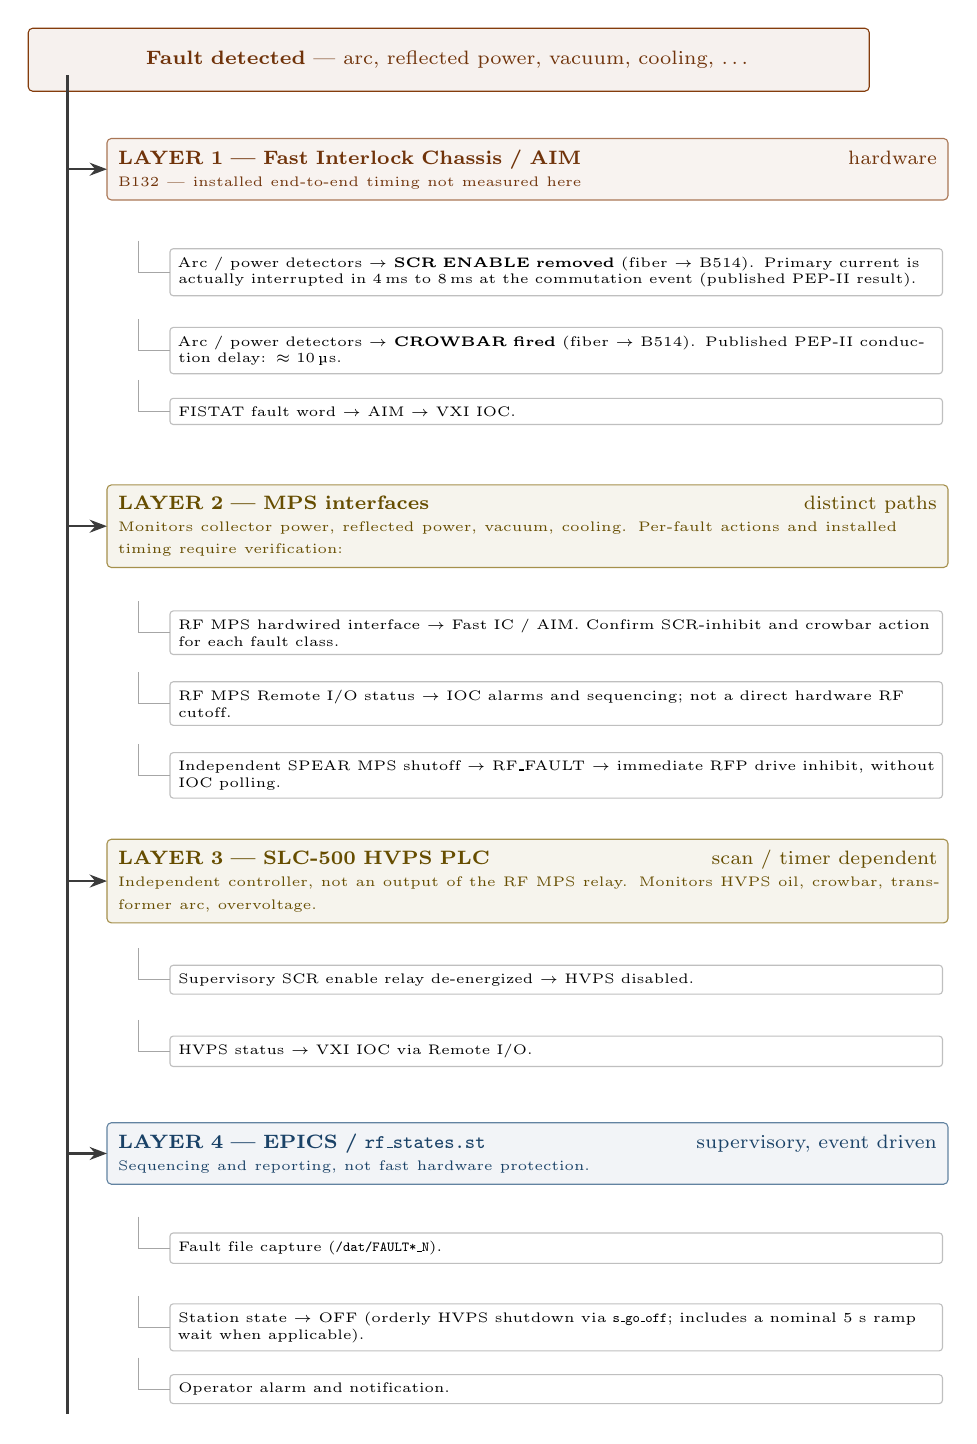
\begin{tikzpicture}[font=\scriptsize,x=1mm,y=1mm,every node/.style={outer sep=0pt}]
\tikzset{act/.style={text width=104mm,anchor=north west,inner sep=4pt,
                     rounded corners=1.6pt,font=\scriptsize,align=left},
         br/.style ={text width=96mm,anchor=north west,inner sep=3pt,
                     font=\tiny,align=left,draw=black!25,fill=white,
                     rounded corners=1.2pt}}

\node[pwr,text width=104mm,anchor=north west] (fault) at (0,0)
  {\textbf{Fault detected} --- arc, reflected power, vacuum, cooling, \dots};

% ---- Layer 1 -------------------------------------------------------------
\node[act,draw=cPwr!70,fill=cPwr!6,text=cPwr!85!black] (l1) at (10,-14)
  {\textbf{LAYER 1 --- Fast Interlock Chassis / AIM} \hfill hardware\\
   {\tiny B132 --- installed end-to-end timing not measured here}};
\node[br] (l1a) at (18,-28)
  {Arc / power detectors $\rightarrow$ \textbf{SCR ENABLE removed} (fiber $\rightarrow$ B514).
   Primary current is actually interrupted in \qtyrange{4}{8}{\milli\second} at the
  commutation event (published PEP-II result).};
\node[br] (l1b) at (18,-38)
  {Arc / power detectors $\rightarrow$ \textbf{CROWBAR fired} (fiber $\rightarrow$ B514).
  Published PEP-II conduction delay: $\approx\qty{10}{\micro\second}$.};
\node[br] (l1c) at (18,-47)
  {FISTAT fault word $\rightarrow$ AIM $\rightarrow$ VXI IOC.};

% ---- Layer 2 -------------------------------------------------------------
\node[act,draw=cPlc!70,fill=cPlc!7,text=cPlc!80!black] (l2) at (10,-58)
  {\textbf{LAYER 2 --- MPS interfaces} \hfill distinct paths\\
   {\tiny Monitors collector power, reflected power, vacuum, cooling.
    Per-fault actions and installed timing require verification:}};
\node[br] (l2a) at (18,-74)
  {RF MPS hardwired interface $\rightarrow$ Fast IC / AIM.
   Confirm SCR-inhibit and crowbar action for each fault class.};
\node[br] (l2b) at (18,-83)
  {RF MPS Remote I/O status $\rightarrow$ IOC alarms and sequencing;
   not a direct hardware RF cutoff.};
\node[br] (l2c) at (18,-92)
  {Independent SPEAR MPS shutoff $\rightarrow$ RF\_FAULT $\rightarrow$
   immediate RFP drive inhibit, without IOC polling.};

% ---- Layer 3 -------------------------------------------------------------
\node[act,draw=cPlc!70,fill=cPlc!7,text=cPlc!80!black] (l3) at (10,-103)
  {\textbf{LAYER 3 --- SLC-500 HVPS PLC} \hfill scan / timer dependent\\
  {\tiny Independent controller, not an output of the RF MPS relay.
    Monitors HVPS oil, crowbar, transformer arc, overvoltage.}};
\node[br] (l3a) at (18,-119)
  {Supervisory SCR enable relay de-energized $\rightarrow$ HVPS disabled.};
\node[br] (l3b) at (18,-128)
  {HVPS status $\rightarrow$ VXI IOC via Remote I/O.};

% ---- Layer 4 -------------------------------------------------------------
\node[act,draw=cCtrl!70,fill=cCtrl!6,text=cCtrl!85!black] (l4) at (10,-139)
  {\textbf{LAYER 4 --- EPICS / \texttt{rf\_states.st}} \hfill supervisory,
  event driven\\ {\tiny Sequencing and reporting, not fast hardware protection.}};
\node[br] (l4a) at (18,-153)
  {Fault file capture (\texttt{/dat/FAULT*\_N}).};
\node[br] (l4b) at (18,-162)
  {Station state $\rightarrow$ OFF (orderly HVPS shutdown via
  \texttt{s\_go\_off}; includes a nominal 5 s ramp wait when applicable).};
\node[br] (l4c) at (18,-171)
  {Operator alarm and notification.};

% ---- spine ---------------------------------------------------------------
% Stubs leave the rail at each layer box's own anchor height, so they are
% exactly horizontal regardless of how tall the box turns out.
\coordinate (rail) at (5,0);
\draw[bus] (5,-6) -- (5,-176);
\foreach \n in {l1,l2,l3,l4}{\draw[sig] (\n.west -| rail) -- (\n.west);}
\foreach \n in {l1a,l1b,l1c,l2a,l2b,l2c,l3a,l3b,l4a,l4b,l4c}
  {\draw[draw=black!35] (\n.west -| 14,0) ++(0,4) -- (\n.west -| 14,0) -- (\n.west);}
\end{tikzpicture}
\end{fitpicture}
\caption{Protection interfaces and supervisory actions.}\label{fig:trip-chain}
\end{figure}

\Cref{fig:interlock-chassis-front} shows the front panel of the Fast Interlock Chassis that implements the hardware layer.

\widefig{interlocak_chassis_front.jpg}{Fast Interlock Chassis 340-308 in B132: reset, filament-timeout and beam-abort controls, channel monitor points, supply-enable indicators and J16 detected-klystron-power input.}{fig:interlock-chassis-front}


\FloatBarrier\clearpage
\part{CONTROL SOFTWARE AND INSTRUMENTATION}


\section{EPICS IOC and SNL Software Architecture}\label{sec:snl-software}

\subsection{IOC Platform}

The VXI crate Slot 0 processor runs VxWorks RTOS with an EPICS IOC. The IOC hosts 6 SNL (State Notation Language) programs compiled into a single \texttt{rfSeq} library:

\begin{longtable}[]{@{}Q{\dimexpr 0.2300\linewidth-1.600\tabcolsep\relax}Q{\dimexpr 0.0879\linewidth-1.600\tabcolsep\relax}Q{\dimexpr 0.1630\linewidth-1.600\tabcolsep\relax}Q{\dimexpr 0.2515\linewidth-1.600\tabcolsep\relax}Q{\dimexpr 0.2676\linewidth-1.600\tabcolsep\relax}@{}}
\toprule\noalign{}
Program & Lines & Instances & Authors & Function \\
\midrule\noalign{}
\endhead
\bottomrule\noalign{}
\endlastfoot
\texttt{rf\_states.st,v} & 2,227 & 1 & R.C. Sass, M. Laznovsky, S. Allison & Master station state machine \\
\texttt{rf\_calib.st,v} & 3,345 & 1 & R. Claus & Calibration sequences \\
\texttt{rf\_tuner\_loop.st,v} & 555 & 4 (per cavity) & --- & Cavity tuner motor control \\
\texttt{rf\_hvps\_loop.st,v} & 343 & 1 & --- & HVPS supervisory control \\
\texttt{rf\_dac\_loop.st,v} & 290 & 1 & S. Allison & Drive/gap voltage DAC control \\
\texttt{rf\_msgs.st,v} & 352 & 1 & --- & Message logging, TAXI monitoring \\
\end{longtable}

The total is \textbf{7,112 source lines}, including comments and blanks, recounted from the RCS head text. The boot script starts nine instances: four tuner instances and one of each other program \R{60}. 


\subsection{rf\_states.st --- Master Station State Machine}

\textbf{Primary States}: OFF (0) → PARK (1) → TUNE (2) → ON\_FM (3) → ON\_CW (4)

\textbf{State architecture}: 3 concurrent state sets:

\begin{enumerate}
\def\labelenumi{\arabic{enumi}.}
\tightlist
\item
  \textbf{\texttt{ss\ rf\_states}} --- 17 states: five operating states plus initialization and transition states
\item
  \textbf{\texttt{ss\ rf\_statesLP}} --- Five states for direct/comb loop switching, gain ramps and beam-abort coordination
\item
  \textbf{\texttt{ss\ rf\_statesFF}} --- One state for asynchronous fault-file export
\end{enumerate}

\textbf{Total}: 23 states across 3 concurrent state sets.

\textbf{State transitions}:

\begin{itemize}
\tightlist
\item
  OFF → PARK: Parks the cavity tuners and coordinates beam-abort reset; initialization is handled separately
\item
  PARK → TUNE: Selects tune mode and starts HVPS/drive sequencing
\item
  TUNE → ON\_FM: Loads the selected 400 Hz or 1 kHz modulation waveform files and enters FM processing mode
\item
  TUNE → ON\_CW: Selects operate-mode references and coordinates the requested loop states; it does not prescribe an RF power level
\item
  Any → OFF: Fault or operator shutdown; orderly disengagement of all loops
\end{itemize}

\subsection{rf\_hvps\_loop.st --- HVPS Supervisory Control}

States: \texttt{init} → \texttt{off} → \texttt{proc} (processing/conditioning) → \texttt{on}

\textbf{Processing mode} carefully ramps HVPS voltage while monitoring cavity vacuum. If vacuum exceeds limits, voltage is reduced. This is used during cavity conditioning and post-trip recovery.

The loop publishes software status codes for operating mode, invalid readbacks, limits and tolerances. These are sequencer-generated statuses, not raw status codes returned by the HVPS hardware \R{17}.

\subsection{rf\_tuner\_loop.st --- Cavity Tuner Control}

Runs as 4 instances (one per cavity) via \texttt{CAV} macro substitution. Implements a slow feedback loop that maintains cavity resonant frequency by:

\begin{enumerate}
\def\labelenumi{\arabic{enumi}.}
\tightlist
\item
  Reading cavity phase angle (from IQA module)
\item
  Comparing against setpoint (optimal detuning for current beam current)
\item
  Commanding stepper motor moves via AB 1746-HSTP1 controller
\end{enumerate}

\textbf{5 SNL states}, 2 control algorithms (phase-feedback-based position tuning for resonance maintenance, and position homing for park/on transitions) plus a loop-off monitoring state.

\subsection{rf\_dac\_loop.st --- Drive/Gap Voltage DAC Control}

Manages the RFP module's octal DACs that control drive power and gap voltage setpoints. The loop operates differently depending on whether the direct feedback loop is on or off, and transitions between TUNE and OPERATE modes.

The four states are \texttt{loop\_init}, \texttt{loop\_off}, \texttt{loop\_tune} and \texttt{loop\_on} \R{77}.

\subsection{rf\_calib.st --- Calibration Sequences}

The largest program, \texttt{P2RF\_Calib} (3,345 lines), has 28 states \emph{including} initialization, completion and abort handling. It calibrates RFP DAC offsets, multipliers, summing/gain stages and modulator/demodulator paths, with PEP-II comb branches retained \R{19}. Cavity resonance, tuner-polynomial and station-response calibrations are separate expert/MATLAB procedures described in \R{8}; they are not all implemented by this sequencer.

\subsection{rf\_msgs.st --- Message Logging}

Two state sets handle software messages and TAXI-link error monitoring (three states total). Log messages are not themselves proof that every associated PV is archived \R{20}.


\section{Tuner Control System}\label{sec:tuner-control}

\subsection{Configuration Currently in Service}\label{sec:tuner-current}

\begin{longtable}[]{@{}P{\dimexpr 0.2831\linewidth-1.000\tabcolsep\relax}P{\dimexpr 0.7169\linewidth-1.000\tabcolsep\relax}@{}}
\toprule\noalign{}
Component & Detail \\
\midrule\noalign{}
\endhead
\bottomrule\noalign{}
\endlastfoot
Controllers & Allen-Bradley 1746-HSTP1 stepper modules (4 units) in chassis 340-315, SN08 \\
Drivers & Superior Electric SLO-SYN SS2000MD4-M PWM step drive translators (one per motor) \\
Motors & Superior Electric SLO-SYN M093-FC11 (NEMA 34D, 4 units) \\
Communication & Allen-Bradley Remote I/O, adapter (rack) 2, from the VXI 6008-SV1R scanner \\
Software & \texttt{rf\_tuner\_loop.st,v} (SNL, 4 instances, 2 Hz) \\
Position feedback & Linear potentiometer per tuner --- indication only \\
\end{longtable}

\subsection{Planned Upgrade Configuration (not yet installed)}

\begin{longtable}[]{@{}P{\dimexpr 0.2894\linewidth-1.000\tabcolsep\relax}P{\dimexpr 0.7106\linewidth-1.000\tabcolsep\relax}@{}}
\toprule\noalign{}
Component & Detail \\
\midrule\noalign{}
\endhead
\bottomrule\noalign{}
\endlastfoot
Controller & Galil DMC-4143 Rev 1.3h 4-axis motion controller in a new SLAC-built chassis \\
Motors & Same SLO-SYN M093-FC11 (retained) \\
Communication & Ethernet (with heartbeat monitoring) \\
Position Feedback & Linear potentiometers on each tuner (retained) \\
\end{longtable}

\textbf{Status.} The Galil controller has been procured and developed on the bench. In August 2025 it was connected to the installed cavity tuner motors and successfully drove them \R{34}; the session log records firmware \texttt{DMC4143\ Rev\ 1.3h}, amplifier \texttt{AMP1\ 43547\ Rev\ 4}, and a series of manual jog and speed tests. \textbf{It has not been installed as the operating controller and is not in the control loop.} It is expected to go online when the LLRF upgrade project completes. Until then the 1746-HSTP1 / SS2000MD4 chain in \cref{sec:tuner-current} is the system of record.

\subsection{Tuner Motion Parameters}\label{sec:tuner-motion}

Values below are defaults in the archived EPICS \texttt{steppermotor} record, device type \texttt{AB-1746HSTP1}. Their units are established by the original record/device support \R{78}. Live values may differ after restoration or operator changes.

\begin{longtable}[]{@{}P{\dimexpr 0.2611\linewidth-1.333\tabcolsep\relax}P{\dimexpr 0.3517\linewidth-1.333\tabcolsep\relax}P{\dimexpr 0.3872\linewidth-1.333\tabcolsep\relax}@{}}
\toprule\noalign{}
Parameter & Value & Record field \\
\midrule\noalign{}
\endhead
\bottomrule\noalign{}
\endlastfoot
Step resolution & 0.003175 mm/step (1.27 mm/rev ÷ 400 steps/rev) & \texttt{DIST} \\
Slew velocity & 3 rev/s = 3.81 mm/s at 1.27 mm/rev & \texttt{VELO}; record conversion uses \texttt{MRES}=400 steps/rev \\
Time to slew velocity & \qty{0.5}{\second} & \texttt{ACCL} (not an acceleration in mm/s$^2$) \\
Upper travel limit & +18 mm & \texttt{DRVH} \\
Lower travel limit & −29.5 mm & \texttt{DRVL} \\
Retry deadband & 0.015875 mm (5 steps) & \texttt{RDBD} \\
Engineering units & mm & \texttt{EGU} \\
Loop rate & 2 Hz & \texttt{rf\_tuner\_loop.st,v} \\
Phase deadband (design) & 0.25° & \texttt{rf\_cav.db,v} \texttt{INPB} (commented out in the DB source) \\
Phase-to-position conversion & 0.020 mm/° in the source comment & \texttt{INPC}; live restored value not supplied \\
Maximum move per cycle & 1 mm in the source comment & \texttt{INPD}; live restored value not supplied \\
\end{longtable}

\begin{keynote}
\textbf{Restore dependency}: The phase deadband, conversion factor, move clamp and outer-loop offset clamp are commented out in the archived database. Without restored nonzero values, the associated correction can be zero. The boot script loads saved records \R{60}, but their live contents are not supplied. Do not infer enabled/disabled loop behavior from either the comments or an absent default alone; verify against the deployed configuration \R{78}.
\end{keynote}

\Cref{fig:rf-mps-plc-modules-allenbradley} shows the adapter and stepper PLC modules.  The motor driver chassis is shown in \cref{fig:cavitytunermotordriver}.

\widefig{rf_mps_plc_modules_allenbradley.jpg}{Allen-Bradley Cavity Tuner Motor Driver chassis (SLAC 340-315, SN08) in the B132 electronics rack --- showing the SLC adapter module (leftmost, with COMM FAULT indicator and STATUS showing RUN/fault) followed by four AB 1746-HSTP1 STEPPER modules (each with RUN, CCW, CW, ERR, FLT indicators; green RUN lights confirm active communication), plus one additional STEPPER module at far right. This chassis is the motion controller currently driving all four cavity tuners; it is to be replaced by the Galil DMC-4143 when the LLRF upgrade project completes}{fig:rf-mps-plc-modules-allenbradley}

\widefig{cavitytunermotordriver.jpg}{Cavity Tuner Motor Driver 340-315, SN08.}{fig:cavitytunermotordriver}


\section{Diagnostics, Calibration and Monitoring}\label{sec:diagnostics}

\subsection{RF Signal Monitoring}

The 24 logical IQA inputs are listed in \cref{sec:iqa-map}. Their physical distribution is described in \cref{sec:waveguide}; the installed connector mapping remains open (O5). Upgrade assignments belong to Doc 0.

\subsection{HVPS Monitoring}

4 analog monitoring signals from B514 to B118 (see \cref{sec:hvps-monitoring-signals}). Additionally, the PLC monitors:

\begin{itemize}
\tightlist
\item
  8 thermocouple channels (4 actively scaled to engineering units)
\item
  Oil level switches (main tank, phase tank, crowbar tank)
\item
  Contactor and grounding switch status
\item
  All fiber optic signal states
\end{itemize}

\subsection{Fault Recording}\label{sec:fault-recording}

\textbf{Configured exports}: The source defines 11 file families, in order: RfpSI, RfpSQ, RfpCI, RfpCQ, CmbI, CmbQ, Iqa1Amp, Iqa2Amp, Gvf, Aim and Iqa3Amp. The \texttt{CF2} compile-time branch substitutes Cf2I/Cf2Q for CmbI/CmbQ; the compiled branch must be checked against the deployed build, not inferred solely from the empty crate slots. \texttt{IQA3MACROS=R=SRF1} in the archived boot script enables the eleventh export request \R{16}, \R{60}.

Exports occur only when fault logging is enabled and \texttt{fault\_detected} is set. \texttt{s\_go\_off} requests them after shutdown sequencing, including a 300-tick (nominally 5 s) voltage-ramp wait when the prior request exceeds 0.1 kV. Hardware histories may already have frozen at the trip. Absent comb/GVF hardware, export errors and timeouts can leave incomplete data; the configured file count is not a guarantee of valid waveforms.

The suffix \texttt{N} is the fault slot number, which cycles \textbf{1 to 15} (\texttt{NUMFAULTS\ =\ 15}) and is published as \texttt{\{STN\}:STN:FAULT:NUM}; the corresponding event timestamps are in \texttt{\{STN\}:STN:FAULT:TIME1} through \texttt{TIME15}. Capture works by temporarily redirecting each module's history-buffer filename and size records (\texttt{MODU.AHFS}, \texttt{MODU.AHSZ}), triggering the dump (\texttt{MODU.GAHS}), waiting on the status field (\texttt{MODU.ASTT}), then restoring the previous filenames and sizes. These files preserve pre-fault waveforms for post-mortem analysis.

\subsection{Calibration Data}

Calibration data include RFP coefficients from \texttt{rf\_calib.st,v} and separately obtained cavity/tuner parameters. The original feedback description \R{8} identifies expert procedures for:

\begin{itemize}
\tightlist
\item
  RF signal amplitude and phase calibration against known references
\item
  Klystron gain curve measurement
\item
  Cavity detuning characterization
\item
  Tuner motor step-to-frequency conversion factors
\end{itemize}


\subsection{Fault Data Availability and Analysis}

The source code describes acquisition capability, not a verified live diagnostic inventory. Four data sources capture fault event information at different time scales.  Summary:

\begin{longtable}[]{@{}P{\dimexpr 0.1543\linewidth-1.500\tabcolsep\relax}P{\dimexpr 0.2595\linewidth-1.500\tabcolsep\relax}P{\dimexpr 0.2149\linewidth-1.500\tabcolsep\relax}P{\dimexpr 0.3713\linewidth-1.500\tabcolsep\relax}@{}}
\toprule\noalign{}
Source & What It Captures & Storage Location & Access \\
\midrule\noalign{}
\endhead
\bottomrule\noalign{}
\endlastfoot
\textbf{AIM hardware history} & Arc-channel/status history, depending on AIM hardware version and configuration & Module memory; export filename is a record setting & Distinguish latched channel bits from analog history; verify installed version and acquisition setup \R{60} \\
\textbf{SNL fault files} (\fpath{/dat/FAULT*_N}) & Up to 11 configured module-history exports; absent modules and errors limit usable data & IOC-visible \fpath{/dat/}; slots 1--15 & Check file existence, timestamps and export status. Configured names are not evidence of valid data \R{16} \\
\textbf{B118 oscilloscope} & Local voltage, current and monitor-winding measurements & Scope setup and saved traces & Confirm channel assignments, triggering and export method in the field; \R{23} is a winding survey, not a scope setup record \\
\textbf{EPICS history service} & Selected PV histories, at configured rates & Controls-managed service & Obtain the channel list, retention and access method from controls. No complete archive configuration is supplied in the cited sources. \\
\end{longtable}

\textbf{Key PVs to check after any fault event}:

\begin{longtable}[]{@{}P{\dimexpr 0.2976\linewidth-1.000\tabcolsep\relax}P{\dimexpr 0.7024\linewidth-1.000\tabcolsep\relax}@{}}
\toprule\noalign{}
PV & Significance \\
\midrule\noalign{}
\endhead
\bottomrule\noalign{}
\endlastfoot
\texttt{\{STN\}:STN:AIM:ARCLTDSTT} & Latched arc-channel mask. Decode using the installed sensor-to-channel map; zero does not exclude a missed, reset or unavailable arc indication. \\
\texttt{\{STN\}:HVPSXFORM:ARC:LTCH} & HV transformer internal arc \\
\texttt{\{STN\}:HVPS:CROWBAR:LTCH} & Crowbar fired \\
\texttt{\{STN\}:STN:MPS:LTCH} & RF MPS PLC trip \\
\texttt{\{STN\}:HVPSSTN:SUMY:LTCH} & Aggregated HVPS fault summary \\
\texttt{\{STN\}:STN:FAULT:NUM} & Fault file slot number (1--15) --- use to locate \fpath{/dat/FAULT*_N} \\
\texttt{\{STN\}:STN:FAULT:TIME1} \ldots{} \texttt{TIME15} & Timestamp of each stored fault event \\
\end{longtable}


\FloatBarrier\clearpage
\part{INTEGRATION AND LEGACY CONSIDERATIONS}


\section{Cabling and Interconnections}

\subsection{Major Cable Runs}

\begin{longtable}[]{@{}P{\dimexpr 0.2250\linewidth-1.500\tabcolsep\relax}P{\dimexpr 0.1925\linewidth-1.500\tabcolsep\relax}P{\dimexpr 0.3351\linewidth-1.500\tabcolsep\relax}P{\dimexpr 0.2474\linewidth-1.500\tabcolsep\relax}@{}}
\toprule\noalign{}
Cable Run & Cable Type & Conductors & Route \\
\midrule\noalign{}
\endhead
\bottomrule\noalign{}
\endlastfoot
B118 → Switchgear (Contactor) & Belden 83715 & 15C \#16 Teflon & TS-5 to contactor controller \\
B118 → Termination Tank (Grounding) & Belden 83709 + Belden 83715 & 9C + 15C \#16 Teflon & TS-6 to grounding tank \\
B118 → B514 (SCR triggers) & Electrical cable pairs & 12 pairs & Controller to Phase Tank thyristor stacks \\
B118 → B514 (Fiber optic) & Fiber optic & SCR ENABLE, CROWBAR, STATUS & Controller to HVPS power section \\
B132 → Tunnel (RF signals) & Coax cables & Forward, reflected, probe per cavity & LLRF inputs from cavities \\
B132 → Tunnel (Motor) & Multi-conductor & Stepper motor phase leads + linear potentiometer feedback per cavity & To tuner assemblies \\
\end{longtable}

\subsection{Connector Types}

\begin{longtable}[]{@{}P{\dimexpr 0.2105\linewidth-1.333\tabcolsep\relax}P{\dimexpr 0.3923\linewidth-1.333\tabcolsep\relax}P{\dimexpr 0.3972\linewidth-1.333\tabcolsep\relax}@{}}
\toprule\noalign{}
Interface & Connector & Notes \\
\midrule\noalign{}
\endhead
\bottomrule\noalign{}
\endlastfoot
PPS & Eight-pin circular connector; exact current type unconfirmed & Identify the installed part and mating/pin convention \R{25}. \\
RF signals & SMA/N-type & 50 Ω coaxial \\
Fiber optic & HFBR series & Avago/Broadcom \\
PLC communication & Allen-Bradley Remote I/O (twinaxial "blue hose") & 6008-SV1R scanner to 1747-DCM / 1771-DCM adapters \\
Galil Ethernet & RJ-45 & Standard Ethernet \\
\end{longtable}


\section{Known Issues}\label{sec:known-issues}

\subsection{Critical Issues}

\begin{longtable}[]{@{}Q{\dimexpr 0.2085\linewidth-1.500\tabcolsep\relax}Q{\dimexpr 0.1005\linewidth-1.500\tabcolsep\relax}Q{\dimexpr 0.1005\linewidth-1.500\tabcolsep\relax}Q{\dimexpr 0.5905\linewidth-1.500\tabcolsep\relax}@{}}
\toprule\noalign{}
Issue & Category & Impact & Details \\
\midrule\noalign{}
\endhead
\bottomrule\noalign{}
\endlastfoot
PPS compliance & Safety & \textbf{Critical} & PLC in PPS chain; PPS wires exposed in HVPS controller enclosure \\
VXI crate obsolescence & Hardware & \textbf{Critical} & Custom SLAC modules (RFP, IQA, CLK, AIM) --- no replacements available. The whole crate is superseded by two Dimtel LLRF9/476 units in the upgrade \R{51}, \R{52} \\
SLC-500 PLC end-of-life & Hardware & \textbf{High} & Allen-Bradley discontinued; no vendor support \\
PLC-5 MPS platform & Hardware & \textbf{High} & Allen-Bradley discontinued; no vendor support \\
SLO-SYN driver obsolescence & Hardware & \textbf{Medium} & SS2000MD4-M discontinued \\
VxWorks/SNL software & Software & \textbf{High} & PEP-II era code (1997); unsupported OS; no modern development tools \\
\end{longtable}

\subsection{Operational Workarounds}\label{sec:operational-workarounds}

The original sources establish the following operating constraints:

\begin{itemize}
\tightlist
\item
  Automatic reset/retry logic exists in \texttt{rf\_states.st,v}, but recovery depends on fault class and configured retry limits \R{16}.
\item
  In-situ automated FM processing is reported at SPEAR3 commissioning \R{1}; the HVPS sequencer also implements vacuum-dependent processing \R{17}. The separate off-line LabVIEW facility in \R{49} is not the station controller. Current conditioning limits and procedures still require approval.
\item
  PEP-II functions (comb filter, GVF/GAP) are absent from the SPEAR3 crate; the station reference is instead supplied by RFP-resident DACs driven by a slow EPICS loop (\cref{sec:feedback-loops})
\item
  Several tuner loop parameters are commented out in the database source and depend on autosave restore to be non-zero (\cref{sec:tuner-motion})
\end{itemize}


\clearpage
\appendix
\section{Source Document Reference Index}\label{appendix-a--source-document-reference-index}

References retain their established IDs and are grouped by source type. 

\subsection{Published Papers and Conference Proceedings}\label{a1-published-papers-and-conference-proceedings}

\begin{longtable}[]{@{}Q{\dimexpr 0.10\linewidth-1.333\tabcolsep\relax}Q{\dimexpr 0.90\linewidth-1.333\tabcolsep\relax}@{}}
\toprule\noalign{}
Ref & Citation \\
\midrule\noalign{}
\endhead
\bottomrule\noalign{}
\endlastfoot
\RDEF{1} & McIntosh, P. et al., "The SPEAR3 RF System," SLAC-PUB-10983, EPAC 2004, pp. 1084--1086. Original proceedings copy: \fpath{llrf/documentation/legacyArchitecture/TUPKF061.pdf}. \url{https://www.osti.gov/biblio/839730} \\
\RDEF{2} & Corredoura, P., "Architecture and Performance of the PEP-II Low-Level RF System," SLAC-PUB-8124, PAC 1999. Original copy: \fpath{llrf/documentation/legacyArchitecture/architecture-and-performance-of-the-pep-ii-low-level-rf.pdf}. \url{https://www.osti.gov/biblio/10204} \\
\RDEF{3} & Corredoura, P., Allison, S., Ross, W., Sass, R., Tighe, R., "Experience with the PEP-II RF System at High Beam Currents," \textbf{SLAC-PUB-8498}, EPAC 2000, arXiv:physics/0007029. \url{https://arxiv.org/abs/physics/0007029} \\
\RDEF{6} & Cassel, R. and Nguyen, M.N., "A Unique Power Supply for the PEP II Klystron at SLAC," SLAC-PUB-7591, PAC 1997. Original: \fpath{hvps/architecture/originalDocuments/slac-pub-7591.pdf}. Published design/test results, not SPEAR3 acceptance data. \url{https://doi.org/10.1109/PAC.1997.753249} \\
\RDEF{45} & Rimmer, R.A., "RF Cavity Development for the PEP-II B Factory," LBL-33360, November 1992. \emph{Cavity design basis for the four SPEAR3 cavities (\cref{sec:cavity-specs}).} \url{https://www.osti.gov/servlets/purl/7066243} \\
\RDEF{46} & Rimmer, R.A. et al., "High-Power Testing of the First PEP-II RF Cavity," UCRL-JC-126198, EPAC 1996, June 1996. Includes the prototype's brief 150 kW test and tuner limitations. \url{https://www.osti.gov/servlets/purl/505666} \\
\RDEF{49} & McIntosh, P., Hill, A. and Schwarz, H., "An Automated 476 MHz RF Cavity Processing Facility at SLAC," SLAC-PUB-10083, PAC 2003. Off-line LabVIEW facility; see \cref{sec:operational-workarounds}. \url{https://www.osti.gov/servlets/purl/815601} \\
\end{longtable}

\subsection{Vendor and Companion References}\label{a2-textbooks-and-general-references}

\begin{longtable}[]{@{}P{\dimexpr 0.0819\linewidth-1.333\tabcolsep\relax}P{\dimexpr 0.9181\linewidth-1.333\tabcolsep\relax}@{}}
\toprule\noalign{}
Ref & Citation \\
\midrule\noalign{}
\endhead
\bottomrule\noalign{}
\endlastfoot
\RDEF{51} & Dimtel, Inc., "LLRF9 Product Page." \emph{The replacement LLRF controller; cited here only to identify what supersedes the VXI system described in \cref{sec:vxi-llrf}.} \url{https://www.dimtel.com/products/llrf9} \\
\RDEF{52} & Dimtel, Inc., "LLRF9/500 Specifications." Vendor-family context, not a specification of the SPEAR3 476 MHz installation. \url{https://www.dimtel.com/products/specs/llrf9_500} \\
\end{longtable}

The companion project reference \R{5} is located in the repository index below for navigation. It is not used as independent confirmation of a disputed original-source claim.

\subsection{Repository Source Index}\label{a3-original-engineering-documents-in-repository}

\begin{longtable}[]{@{}P{\dimexpr 0.0758\linewidth-1.333\tabcolsep\relax}P{\dimexpr 0.5035\linewidth-1.333\tabcolsep\relax}P{\dimexpr 0.4207\linewidth-1.333\tabcolsep\relax}@{}}
\toprule\noalign{}
Ref & Document & Repository Path \\
\midrule\noalign{}
\endhead
\bottomrule\noalign{}
\endlastfoot
\RDEF{4} & LLRF9 Commissioning Tests (J. Sebek, 2021) --- source of the \textasciitilde712 kV/cavity operating gap voltage & \fpath{llrf/tests/llrf9Tests.pdf}, \fpath{llrf/tests/llrf9Tests.tex} \\
\RDEF{5} & Project Physical Design Report R2 (28 April 2026); current companion Doc 0 is R3 (25 September 2026) & \fpath{Designs/docx/SPEAR3_LLRF_PDR_R2.docx}; \fpath{Designs/tex/doc0-system-design/0_system_design_report.pdf} \\
\RDEF{7} & PEP-II RF System Description (Schwarz, PS-340-330-51-R0) --- cavity R\_s, Q\_0, β & \fpath{llrf/documentation/legacyArchitecture/ps3403305100.pdf} \\
\RDEF{8} & LLRF Feedback Loop Description (Schwarz, PS-340-330-52-R0) & \fpath{llrf/documentation/legacyArchitecture/ps3403305200.pdf} \\
\RDEF{9} & HVPS System Schematic (top-level) & \fpath{hvps/documentation/schematics/sd7307900101.pdf} \\
\RDEF{10} & LLRF Block Diagram (HER configuration) & \fpath{llrf/documentation/legacyArchitecture/bd3403300000.pdf} \\
\RDEF{11} & LLRF Block Diagram (alternative view) & \fpath{llrf/documentation/legacyArchitecture/bd3403300100.pdf} \\
\RDEF{12} & Analog Regulator Card Schematic & \fpath{hvps/documentation/schematics/sd2372301401.pdf} \\
\RDEF{13} & \textbf{Enerpro General Purpose 3-Phase Firing Circuit, PCB PN FCOG6100} --- SLAC SD-237-230-12-R0 / Enerpro drawing E128, drawn W.C. Mitchell 9/29/87. \emph{This file is \textbf{not} a voltage-divider drawing, despite having been catalogued as one; the dividers are on \R{71}.} & \fpath{hvps/documentation/schematics/sd2372301200.pdf} \\
\RDEF{14} & Interconnection: B118 ↔ Contactor ↔ Termination Tank & \fpath{hvps/documentation/wiringDiagrams/wd7307900103.pdf} \\
\RDEF{15} & Hoffman Box Internal Wiring & \fpath{hvps/documentation/wiringDiagrams/wd7307900206.pdf} \\
\RDEF{16} & Legacy SNL: rf\_states.st (master state machine) & \fpath{spear-rf-code-legacy/rfApp/src/seq/rf_states.st,v} \\
\RDEF{17} & Legacy SNL: rf\_hvps\_loop.st (HVPS control) & \fpath{spear-rf-code-legacy/rfApp/src/seq/rf_hvps_loop.st,v} \\
\RDEF{18} & Legacy SNL: rf\_tuner\_loop.st (tuner control) & \fpath{spear-rf-code-legacy/rfApp/src/seq/rf_tuner_loop.st,v} \\
\RDEF{19} & Legacy SNL: rf\_calib.st (calibration sequences) & \fpath{spear-rf-code-legacy/rfApp/src/seq/rf_calib.st,v} \\
\RDEF{20} & Legacy SNL: rf\_msgs.st (message logging) & \fpath{spear-rf-code-legacy/rfApp/src/seq/rf_msgs.st,v} \\
\RDEF{21} & MPS Wiring Diagrams (33 drawings) & \fpath{llrf/documentation/mpsWiringDiagrams/wd3403300200.pdf} through \texttt{wd3403303400.pdf} \\
\RDEF{22} & PEP-II HVPS Technical Specification (PS-341-360-01-R2) & \fpath{hvps/architecture/originalDocuments/ps3413600102.pdf} \\
\RDEF{23} & HVPS monitor-winding connection/resistance surveys, separate sheets for HVPS1 and HVPS2; not an oscilloscope setup record & \fpath{hvps/documentation/wiringDiagrams/hvpsMonitorConnections.xlsx} \\
\RDEF{24} & HVPS Measurements (March 2022) & \fpath{hvps/documentation/plc/hvpsMeasurements20220314.xlsx} \\
\RDEF{25} & PPS Wiring in Hoffman Box (J. Sebek) --- terminal-by-terminal PPS trace, PLC rung analysis, switchgear theory of operation, K4/RR label finding & \fpath{pps/HoffmanBoxPPSWiring.docx} \\
\RDEF{26} & PLC Ladder Logic Printout (Cassel) & \fpath{hvps/documentation/plc/CasselPLCCode.pdf} \\
\RDEF{27} & PLC Symbol/Label Database (Cassel) & \fpath{hvps/documentation/plc/CasselSymbolDatabase.pdf} \\
\RDEF{28} & Enerpro Schematics and Manuals (12 PDFs) & \fpath{hvps/controls/enerpro/enerproDocuments/} \\
\RDEF{29} & SLO-SYN Stepper Drive Manual & \fpath{llrf/tuners/SLO-SYN_SS2000MD4M_Step_Drive_Translator_Manual.pdf} \\
\RDEF{30} & SLO-SYN Motor Specifications & \fpath{llrf/tuners/SLO-SYN.pdf} \\
\RDEF{31} & Galil DMC-41x3 series user manual (covers the DMC-4143) & \fpath{llrf/tuners/galil/dmc-4103-r13h-manual.pdf}; datasheet \fpath{llrf/tuners/galil/ds_41x3.pdf} \\
\RDEF{32} & Drive Amplifier Datasheet (KAW2051M12) & \texttt{llrf/driveAmp/KAW2051M12\ (7-98-907-012A).pdf} \\
\RDEF{33} & Coaxial Cable Interconnection Diagram & \fpath{llrf/documentation/coaxCables/sd3403300100.pdf} \\
\RDEF{34} & Galil bench session log with the installed cavity motors (25 Aug 2025) --- records firmware \texttt{DMC4143\ Rev\ 1.3h}, \texttt{AMP1\ 43547\ Rev\ 4} & \fpath{llrf/tuners/galil/functioningGalil20250825SwapABToManual.txt}; earlier session \texttt{firstMotion2024.txt} \\
\RDEF{35} & Galil Commissioning Documentation & \fpath{llrf/tuners/galil/GalilCommissioning.docx} \\
\RDEF{36} & Cavity Tuner Inspections (June 2023) & \fpath{llrf/tuners/cavityTunerInspections20230613.docx} \\
\RDEF{37} & PLC Operation Notes & \fpath{hvps/documentation/plc/plcNotesR1.docx} \\
\RDEF{38} & PLC Software Discussion & \texttt{hvps/documentation/plc/PLC\ software\ discusion\ 1.docx} \\
\RDEF{39} & PLC Label Database & \fpath{hvps/documentation/plc/hvpsPlcLabels.xlsx} \\
\RDEF{40} & Enerpro Modifications for SLAC HVPS (J. Sebek) --- installed FCOG6100/FCOAUX60 identity and serial numbers, phase-reference measurements, SIG HI summing chain & \fpath{hvps/controls/enerpro/enerproBoardHvps.docx} \\
\RDEF{53} & Dusatko, J., \emph{The SPEAR3 Low Level RF System Description}, v1.2, 4 May 2004, updated 29 January 2016. Component/clock description; historical crate and ripple statements require the reconciliations in \cref{sec:vxi-llrf} & \fpath{llrf/documentation/legacyArchitecture/SP3_writeup_V1d2.pdf} \\
\RDEF{54} & Ross, W., \emph{PEP-II/SPEAR3 LLRF System Clock Module Revision 2}, SLAC ESD Engineering Document, 1 September 2001 & Cited as reference 3 of \R{53}; document not held in this repository \\
\RDEF{56} & Sebek, J., \emph{SPEAR3 High Voltage Power Supply Hazards}. Source of operating snapshots and discharge models; Doc L corrects its T0-rating inference and output-energy sum & \fpath{hvps/documentation/procedures/spear3HvpsHazards.tex} \\
\RDEF{58} & Sebek, J., \emph{Enerpro Phase Reference Adapter} --- the upgrade adapter design (576 kΩ / 200 kΩ into FCOG1200 J7) & \fpath{hvps/controls/enerpro/enerproPhaseReferenceAdapter.docx} \\
\RDEF{60} & Legacy IOC boot and Remote I/O configuration & \fpath{spear-rf-code-legacy/iocBoot/b132-iocrf/st.cmd,v}, \texttt{config.ab,v}; \fpath{spear-rf-code-legacy/rfApp/DbIoc/srf1.substitutions,v}; \fpath{spear-rf-code-legacy/rfApp/Db/rf_ab_4CV.substitutions,v}; \fpath{spear-rf-code-legacy/rfApp/src/db/p2RfAimDef.h,v}; \fpath{spear-rf-code-legacy/allenBradley/documentation/allenBradley.html,v} \\
\RDEF{61} & SCR trigger, interlock and monitor board schematics (SD-730-793 series) --- verified by direct reading of the scanned drawings, September 2026 & \fpath{hvps/documentation/schematics/sd7307930304.pdf}, \texttt{sd7307930402.pdf}, \texttt{sd7307930702.pdf}, \texttt{sd7307930801.pdf}, \texttt{sd7307931203.pdf}, \texttt{sd7307931301.pdf} \\
\RDEF{62} & Grounding Tank schematic, SD-730-790-05-C1 (R. Cassel, 2/13/03) --- verified by direct reading, September 2026 & \fpath{hvps/documentation/schematics/sd7307900501.pdf} \\
\RDEF{63} & \textbf{Trigger Enclosure Wiring, WD-730-790-02-C6} (R. Cassel / W. Gorecki / S. Lowe; revisions C1--C6, 06/03 to 01/07) --- master wiring diagram for the B118 trigger enclosure; verified by direct reading, September 2026 & \fpath{hvps/documentation/wiringDiagrams/wd7307900206.pdf} \\
\RDEF{64} & Grounding Tank Wiring, WD-730-794-06-C0 (R. Cassel / W. Gorecki 03/03/2000 / S. Lowe 4/3/00) --- \textbf{test stand} configuration, no revisions recorded; verified by direct reading, September 2026 & \fpath{hvps/documentation/wiringDiagrams/wd7307940600.pdf} \\
\RDEF{65} & Vacuum Contactor Controller Electrical Schematic, GP-439-704-02-C1 (redrawn to CAD per as-built, 09/25/06) --- verified by direct reading, September 2026 & \fpath{hvps/documentation/switchgear/gp4397040201.pdf} \\
\RDEF{66} & Ross Engineering 713203 E-1, High Speed Vacuum Contactor Energy Storage Closing \& Holding System Schematic (driver HCA-1-A P/N 820360; contactor HQ3 P/N 813203; last revision E, 2-2-83) --- verified by direct reading, September 2026 & \fpath{hvps/documentation/switchgear/rossEngr713203.pdf} \\
\RDEF{67} & \textbf{Interconnection Wiring, WD-730-790-01-C3} (R. Cassel / W. Gorecki 03/02/2000 / S. Lowe; revisions C1--C3, 08/03 to 10/03) --- system-level interconnection between the B118 Hoffman Box, Contactor Disconnect and Termination Tank; verified by direct reading, September 2026 & \fpath{hvps/documentation/wiringDiagrams/wd7307900103.pdf} \\
\RDEF{68} & \textbf{12.47 kV Vacuum Contactor Controller, Electrical Connection Wiring Diagram, ID-308-801-06-C1} (redrawn to CAD and resized D→E, revised per as-built, 09/25/06; supersedes ID-308-801-06 R0) --- the connection-wiring companion to \R{65}; verified by direct reading, September 2026 & \fpath{hvps/documentation/switchgear/id3088010601.pdf} \\
\RDEF{69} & \textbf{12.47 kV Outdoor Metal-Enclosed Combination Vacuum Contactor Controller --- Schematic Diagram \& General Arrangement, GP-308-500-01-R3} (Lawrence Berkeley Laboratory; A. Tseng / L. Johnson, 6-23-77, revisions 1--3) --- the original PEP-era design drawing; authoritative source for the relay device legend; verified by direct reading, September 2026 & \fpath{hvps/documentation/switchgear/gp3085000103.pdf} \\
\RDEF{70} & \textbf{Klystron Power Supply Electrical Schematic, EI-730-790-00-C0 / NWL \# 39308} (NWL Transformers, Bordentown NJ; SLAC issue R. Cassel / W. Gorecki 12/17/02 / J. Olszewski 1/21/03; NWL revisions A--F, 1996--2001) --- the \textbf{transformer manufacturer's own schematic}; authoritative for transformer ratings, monitor windings and oil/pressure protection setpoints; verified by direct reading, September 2026 & \fpath{hvps/documentation/wiringDiagrams/ei7307900000.pdf} \\
\RDEF{71} & \textbf{SCR Control Driver --- Crowbar Interconnecting Cables, WD-730-794-04-C0} (R. Cassel 5/30/00 / W. Gorecki 03/03/2000 / S. Lowe 4/3/00) --- contains the \textbf{"TRANSFORMER TANK WD-730-792-01"} section with both HVPS output voltage dividers, the crowbar trigger transformer T1 feeding SCR1--SCR4 over RG-220, and the CR1--CR4 driver board pinouts; verified by direct reading, September 2026 & \fpath{hvps/documentation/wiringDiagrams/wd7307940400.pdf} \\
\RDEF{72} & \textbf{Enerpro Voltage and Current Regulator Board Notes} --- J. Sebek. Detailed circuit analysis of SD-237-230-14-C1: divider loading and transfer functions, error-amplifier pole/zero analysis, the diode minimum-select summing junction, and the finding that the AC current loop is saturated by design & \fpath{hvps/architecture/designNotes/EnerproVoltageandCurrentRegulatorBoardNotes.docx} \\
\RDEF{75} & \textbf{NWL transformer rating plate, SPEAR2 unit} --- the manufacturer's nameplate on the transformer tank, photographed in place September 2026; primary source for the unit's own ratings and for the NWL model and drawing numbers & \fpath{Designs/tex/common/photos/SPEAR2\_HVPS\_Plate.jpg} \\
\RDEF{76} & Original IQA channel allocation, instantiated by the SPEAR3 station database & \fpath{spear-rf-code-legacy/rfApp/Db/rf_iqa_All.substitutions,v}; \fpath{spear-rf-code-legacy/rfApp/Db/rf_iqa_4CV.substitutions,v} \\
\RDEF{77} & Legacy DAC supervisory loop & \fpath{spear-rf-code-legacy/rfApp/src/seq/rf_dac_loop.st,v} \\
\RDEF{78} & Original tuner database, stepper record definition and conversion code, and AB device support & \fpath{spear-rf-code-legacy/rfApp/Db/rf_cav.db,v}; \fpath{spear-rf-code-legacy/stepper/stepper/steppermotorRecord.dbd,v}; \fpath{spear-rf-code-legacy/stepper/stepper/steppermotorRecord.c,v}; \fpath{spear-rf-code-legacy/allenBradley/allenBradleyApp/1746HSTP1Src/devSmAB1746HSTP1.c,v} \\
\RDEF{79} & Original Fast Interlock Chassis, receiver-board and interface-module schematics; drawing revision is not proof of installed configuration & \fpath{llrf/documentation/legacyInterfaceModules/SD-340-308-01-R1-1of1.pdf}; \fpath{llrf/documentation/legacyInterfaceModules/SD-340-308-02-R1.pdf}; \fpath{llrf/documentation/legacyInterfaceModules/sd3403090102.pdf} \\
\RDEF{80} & \textbf{SCR Control Driver --- Contactor Interconnecting Cables, WD-730-794-02-C0} (R. Cassel / W. Gorecki 03/03/2000 / S. Lowe 4/2/00) --- the TS-5 conductor list and the contactor-disconnect terminal layout, including the MX, RR and K-4 coil connections; verified by direct reading, October 2026 & \fpath{hvps/documentation/wiringDiagrams/wd7307940200.pdf} \\
\end{longtable}

\clearpage
\section{Symbol and Notation Conventions}\label{appendix-b--symbol-and-notation-conventions}

\subsection{Frequently Used Symbols}\label{b1-frequently-used-symbols}

\begin{longtable}[]{@{}lll@{}}
\toprule\noalign{}
Symbol & Definition & Typical Unit \\
\midrule\noalign{}
\endhead
\bottomrule\noalign{}
\endlastfoot
$f_0$, $\omega_0$ & Cavity resonant frequency & MHz, rad/s \\
$f_\text{RF}$, $\omega_\text{RF}$ & RF operating frequency (\textasciitilde476.3 MHz, drifting --- \cref{sec:rf-parameters}) & MHz, rad/s \\
$f_\text{rev}$, $\omega_\text{rev}$ & Revolution frequency (\textasciitilde1.2804 MHz) & MHz, rad/s \\
$f_s$, $\omega_s$ & Synchrotron frequency (\textasciitilde10.1 kHz) & kHz, rad/s \\
$Q_0$ & Unloaded quality factor (32,000) & dimensionless \\
$Q_L$ & PEP-II nominal loaded quality factor (\textasciitilde6,780) & dimensionless \\
$\beta$ & Coupling coefficient $= Q_0/Q_\text{ext}$ (PEP-II nominal 3.72) & dimensionless \\
$R_s$ & Shunt impedance (3.73 M$\Omega$, linac convention) & M$\Omega$ \\
$V_\text{gap}$ & Gap voltage per cavity (\textasciitilde712 kV operating) & kV \\
$I_b$ & DC beam current (500 mA design) & mA or A \\
$V_\text{HV}$ & HVPS output voltage ($\approx$ \qtyrange{-72}{-75}{\kilo\volt} typical) & kV \\
$I_\text{HV}$ & HVPS output current ($\approx$ \qtyrange{19}{22}{\ampere} typical) & A \\
$\alpha$ & SCR firing angle & degrees \\
SIG HI & Enerpro firing-angle command voltage; calibrated mapping required & V \\
\end{longtable}

\subsection{Abbreviations}\label{b2-abbreviations}

\begin{longtable}[]{@{}P{\dimexpr 0.2075\linewidth-1.000\tabcolsep\relax}P{\dimexpr 0.7925\linewidth-1.000\tabcolsep\relax}@{}}
\toprule\noalign{}
Abbreviation & Definition \\
\midrule\noalign{}
\endhead
\bottomrule\noalign{}
\endlastfoot
AIM & Arc/Interlock Module (VXI slot 12, SLAC drawing 340-307) \\
CLK & Clock/RF Distribution module (VXI slot 2) \\
DCM & Direct Communication Module --- an Allen-Bradley \textbf{Remote I/O adapter} (1747-DCM for SLC-500, 1771-DCM for PLC-5) \\
Fast IC & Fast Interlock Chassis (SLAC drawing 340-308) \\
GVF / GAP & Gap Voltage Feed-Forward (PEP-II only; module not installed in SPEAR3) \\
HER & High Energy Ring (PEP-II) \\
HOM & Higher-Order Mode \\
HVPS & High-Voltage Power Supply \\
IQA & IQ/Amplitude detector module (VXI slots 7, 9, 11) \\
LLRF & Low-Level RF \\
MPS & Machine Protection System (RF MPS = the station-level equipment protection PLC; SPEAR MPS = the facility system) \\
PPS & Personnel Protection System \\
RFP & RF Processor module (VXI slot 4) \\
RIO & Allen-Bradley Remote I/O --- the serial link between the VXI 6008-SV1R scanner and the PLC adapters \\
SCR & Silicon Controlled Rectifier (thyristor) \\
SNL & State Notation Language (EPICS) \\
\end{longtable}

\subsection{Conventions}\label{b3-conventions}

\begin{enumerate}
\def\labelenumi{\arabic{enumi}.}
\item
  \textbf{Shunt impedance}: $R_s=V_{\mathrm{gap,pk}}^2/(2P_{\mathrm{wall}})$, approximately \qty{3.73}{\mega\ohm} in the PEP-II nominal table \R{7}. McIntosh's \qty{3.8}{\mega\ohm} SPEAR3 value uses the same definition \R{1}. The alternative $V_{\mathrm{gap,pk}}^2/P_{\mathrm{wall}}$ definition is twice as large. 
\item
  \textbf{Phase convention}: Positive phase angles represent phase advance. The synchronous phase $\varphi_s$ is measured from the zero-crossing of the RF voltage.
\item
  \textbf{Frequency detuning}: $\Delta f = f_0 - f_\text{RF}$. Negative detuning ($\Delta f < 0$) means the cavity resonant frequency is below the RF frequency, which is the normal operating condition for beam loading compensation above transition.
\item
  \textbf{Reference tag format}: {[}Rn{]} for numbered references, {[}Wn{]} for web references.

\end{enumerate}



\emph{End of Document}




\end{document}
